% !TEX encoding = UTF-8 Unicode
% !BIB TS-program = biber 
% !BIB program = biber    

% This file is MIT-Thesis.tex, a LaTeX template for formatting an MIT thesis with the mitthesis class.
%
% Version: 1.11, 2023/11/02
%
% Author: John H. Lienhard, copyright 2023. Reuse under the MIT license: https://ctan.org/license/mit 

% Documentation is here: https://ctan.org/pkg/mitthesis

%% Don't modify the \DocumentMetadata command unless you know what it does. 
%% If this command throws an "undefined" error, your latex system is out of date: try commenting this command out.
\DocumentMetadata{ 
	pdfstandard = a-2b,
	pdfversion  = 1.7,
	lang		= en-US,
%	debug		= {xmp-export}, % uncomment to output a separate xmpi file showing the metadata
}
%%%%%%%%%%%%%%%%%%%%%%%%%%%%%%%%%%%%%%%

\documentclass[twoside]{mitthesis} %,fontset=libertine, fontset=newtx-sans-text, fontset=heros-stix2, fontset=stix2
%
% option [twoside]		gives facing-page behavior for printing; omitting twoside will eliminate even-numbered blank pages.
% option [lineno]	 	provides line numbers, as for editing
% option [mydesign] 	loads packages for color, title and list formats, margins, or captions: edit mydesign.tex to change defaults.
% option [fontset] is a keyvalue which can be:
%					 	pdftex or unicode engines:  defaultfonts, libertine, lucida
%					 	pdftex only: 				fira-newtxsf, newtx, newtx-sans-text
%						unicode engines (luatex):	heros-stix2, stix2, termes, termes-stix2
%					 	if no key value is given, fonts default to CMR (pdftex) or LMR (unicode), i.e., "the LaTeX font".
%					 	You can edit the fontset files or you can write your own, myfonts.tex, and do [fontset=myfonts].
%						If you are using multiple languages, load the babel package in your fontset file, before the fonts.

%%%%%%%%% Packages used in sample chapters (not otherwise required) %%%%%%%

%% Package for code listing in Appendix A.
\usepackage{listings}%   documentation is here https://ctan.org/pkg/listings

%% Set chemical formulas nicely
\usepackage[version=4]{mhchem}%   documentation is here https://ctan.org/pkg/mhchem

%% Latin filler used in Chapter 1, with a test for package version date. https://ctan.org/pkg/lipsum
\usepackage{lipsum}
\IfPackageAtLeastTF{lipsum}{2021/09/20}{\setlipsum{auto-lang=false}}{}

% Packages installed by Julius
\usepackage{braket}     % for \braket{}, \ket{}, \bra{}
\usepackage{cancel}     % for \cancel{}
\usepackage{tabularx}
\usepackage{enumitem}
\usepackage{amsmath}
\usepackage{float}


%%%%%%%%%  Graphics path (to figure files)  %%%%%%%%%%%%%%%%%%%%%%%%%%%%%%%%

%% Can set graphicspath to point to specific directories containing figures (the current directory is searched automatically)
%% For instance, to search a subdirectory of the current directory called "figures" and a parallel directory called "art", set:

% \graphicspath{ {figures/} {../art/} }% For details see: https://latexref.xyz/dev/latex2e.html#g_t_005cgraphicspath


%%%%%%%%%  Representative set-up for biblatex  %%%%%%%%%%%%%%%%%%%%%%%%%%%%%

%\usepackage[style=ieee,maxbibnames=10,sorting=none]{biblatex}% style=ext-numeric-comp,articlein=false,giveninits=true
%	\DefineBibliographyStrings{english}{url= \textsc{url} ,  }% replaces default "[Online]. Available" by "URL"


% \addbibresource{mitthesis-sample.bib}%% <== change to YOUR bib file <= CHANGE

%% to avoid split urls and stretched white space, you can set the bibliography ragged-right:
% \appto{\bibsetup}{\raggedright}

% biblatex is very powerful, and you can customize most aspects the reference list and citations to suit your needs.
% documentation is here: https://ctan.org/pkg/biblatex


%%%%%%%%%%  Option to use natbib   %%%%%%%%%%%%%%%%%%%%%%%%%%%%%%%%%%%%%%%%%

\RequirePackage[numbers,sort&compress]{natbib}
 
%%% add bibliography to table of contents
\apptocmd{\bibliography}{\addcontentsline{toc}{chapter}{\protect\textbf{\bibname}}}{}{}

%%% You can use this to rename the bibliography section
\renewcommand{\bibname}{References}

%%% Can adjust space between bibliography items (change 4pt to something else; don't drop last two lengths, they are stretchable "glue")
\setlength\bibsep{4pt plus 1pt minus 1pt}


%%%%%%%%%%  Table related packages  %%%%%%%%%%%%%%%%%%%%%%%%%%%%%%%%%%%%%%%%

\usepackage{booktabs}% better quality tables, https://ctan.org/pkg/booktabs
\usepackage{array}%    additional options for table columns, https://ctan.org/pkg/array

%\usepackage{tabularx}%   https://ctan.org/pkg/tabularx

%\usepackage{dcolumn}%    alignment on decimal place, https://ctan.org/pkg/dcolumn
%\newcolumntype{d}[1]{D{.}{.}{#1}}


%%%%%%%%%%  Option for "double spacing" %%%%%%%%%%%%%%%%%%%%%%%%%%%%%%%%%%%%

%% Back in the typewriter era, double spaced lines were convenient for editing with a pencil. 
%% In typography, the separation between lines is called "leading", and it is usually set in 
%% proportion to the font size (i.e., when the font is loaded).  If you really feel the need 
%% to change the line separation, the most attractive results will be obtained by changing the
%% leading in proportion to the the current font size, rather than just doubling the space.

%% The setspace package provides a tool for changing line separation. Use these two commands here:
%
% \usepackage{setspace}%  documentation at https://ctan.org/pkg/setspace
% \setstretch{1.1}% you can choose some other value for the stretch of space between lines
%
%% Use one or more of the these commands AFTER the frontmatter
%
% \onehalfspacing
% \doublespacing
% \singlespacing  % will turn these effects off (you can use these anywhere in the document)

%% The best result may be to stay with leading selected by the typographer who set up the font.


%%%%%%%%%%%  Metadata  %%%%%%%%%%%%%%%%%%%%%%%%%%%%%%%%%%%%%%%%%%%%%%%%%%%%%%%

% Most of the document metadata is created automatically. 
% The following items should be adjusted to match your work. <================= !!!!!!!!!!

\hypersetup{%
	pdfsubject={Template for writing MIT theses with the mitthesis class},
	% Change this to briefly state topic of your thesis 
% 
	pdfkeywords={Massachusetts Institute of Technology, MIT},
	% Add keywords that will help search engines and libraries to find your work.
	% Includes the name[s] of the author[s] 
	% (If you have used \DocumentMetadata, at line 15, you can just put "\CopyrightAuthor," for the names.)
%
	pdfurl={},
	% If you have a url for the thesis, put it here. Otherwise delete this.
	% (MIT Libraries will put your thesis in DSPACE with a persistent url after you submit it.)
%	
	pdfcontactemail={},
	% You can put a [permanent] email address into the metadata, if you like.
	% Otherwise delete this.
%
	pdfauthortitle={},
	% If you have a title, you can include it here.
}

%%%%%%%%%%%%%%  End preamble %%%%%%%%%%%%%%%%%%%%%%%%%%%%%%%%%%%%%%%%%%%%%%%%%%%%%%%%%%%%%%%%%%%%%
%%%%%%%%%%%%%%%%%%%%%%%%%%%%%%%%%%%%%%%%%%%%%%%%%%%%%%%%%%%%%%%%%%%%%%%%%%%%%%%%%%%%%%%%%%%%%%%%%%

\begin{document}

%%% edit the following commands to match your thesis %%%%%%%%%%

\title{Search for Rare Charm Decays into Two Muons}

% \Author{Author full name}{Author department}[Author's first PREVIOUS degree][Author's second PREVIOUS degree][...
% Note that third, fourth, fifth, and sixth arguments are optional [] and may be omitted

% note on names: most of the following names are made up; Silas Holman was a physics professor at MIT in the 19th century.

\Author{Julius Heitkoetter}{Department of Physics}
% \Author{Luisa Hernández}{Department of Research}[B.S. Mechanical Engineering, UCLA, 2018][M.S. Stellar Interiors, Vulcan Science Academy, 2020]
% \Author{Thurston Howell III}{Department of Economics}[MBA, Ferengi School of Management, 2022]

% Use once for each degree fulfilled by thesis
% For two degrees from one department, leave the department argument blank for the second degree {}.
% \Degree{Bachelor of Science in Physics}{Department of Physics}
% \Degree{Master of Science in Physics}{}
\Degree{Bachelor of Science in Physics}{Department of Physics}

% If there is more than one supervisor, use the \Supervisor command for each.
\Supervisor{Christoph Paus}{Professor of Physics}
% \Supervisor{Secunda Castor}{Professor of Research}
% \Supervisor{Quintus Castor}{Professor of Log Dams}

% Professor who formally accepts theses for your department (e.g., the Graduate Officer, Professor Sméagol,...)
% If more than one department, use more than once
% **If you need to reduce vertical space, put the acceptor title in the second argument and leave the third blank {}.**
 \Acceptor{Lindley Winslow}{Associate Professor of Physics}{Associate Head, Department of Physics}
% \Acceptor{Tertius Castor}{Professor of Log Dams}{Graduate Officer, Department of Research}
% \Acceptor{Quarta Castor}{Professor of Lodge Building}{Graduate Officer, Department of Mechanical Engineering}

% Usage: \DegreeDate{Month}{year}
% Valid degree months are September, February, or June
\DegreeDate{June}{2025}

% Date that final thesis is submitted to department
\ThesisDate{May 9, 2025}

%%%%%%  Choose whether to have a CREATIVE COMMONS License  %%%%%%%%%%%%%%%%%%%%%%%%%%%%%%%%%%%%%%
%
% If you are using a cc license, put details of your cc license here. 
% Omit this command if you are not using a cc license.
%
\CClicense{CC BY-NC-ND 4.0}{https://creativecommons.org/licenses/by-nc-nd/4.0/}
%

%%%%%%%  Solutions for overflowing titlepage  %%%%%%%%%%%%%%%%%%%%%%%%%%%%%%%%%%%%%%%%%%%%%%%%%%%

% If your title page is overflowing (from too many names, degrees, etc.):
%
% (a) you can reduce the 12pt and 18pt skips between various blocks to 6pt with this command:
%
% \Tighten
%
% (b)  you can scale down the Signature block at the bottom with this command:
%
% \SignatureBlockSize{\small}  %or this one \SignatureBlockSize{\footnotesize}
%
% (c) you can put the acceptor name and title onto two lines, rather than three like this:
%
% \Acceptor{Tertius Castor}{Professor and Graduate Officer, Department of Research}{}
% \Acceptor{Quarta Castor}{Professor and Graduate Officer, Department of Mechanical Engineering}{}
%
% (d) you can change the font size of the the author name[s] with
%
%	\AuthorNameSize{\normalsize}
%
% (e) and you can omit any previous degrees from the title page, instead mentioning them in the Biosketch

% Also, if you prefer to keep the text toward the top of the page with most white space at the bottom, you
% can you this command to squash all of the vertical glue (stretchy space) with this command:
%
% \Squash 
%
% This command is useful when the text has not already reach the bottom of the page, since the glue gets squashed automatically
% when the page is too full.

%%%%%%%%%%%%%%%%%%%%%%%%%%%%%%%%%%%%%%%%%%%%%%%%%%%%%%%%%%%%%%%%%%%%%%%%%%%%%%%%%%%%%%%%%%%%%%%%%

%%% Make titlepage
\maketitle

%%%%%%%%% Contents that you need to write follows %%%%%%%%%%%%%%%%%%%%%%%%%%%%%%%%%%%%%%%%%%%%%%%%

% \includeonly{acknowledgments,biography,chapter1,chapter2,...,appendixa,...} 
%   for usage, see https://latexref.xyz/_005cinclude-_0026-_005cincludeonly.html

%%% Frontmatter (write this material in the mentioned files)  %%%%%%%%%%%%%%%%%%%%%%%%%%%%%%%%%%%%

% The abstract environment creates all the required headings and footers. 
% You only need to the text of the abstract in the file abstract.tex
\begin{abstract}
	% From mitthesis package
% Version: 1.01, 2023/06/19
% Documentation: https://ctan.org/pkg/mitthesis
%
% The abstract environment creates all the required headers and footnote. 
% You only need to add the text of the abstract itself.
%
% Approximately 500 words or less; try not to use formulas or special characters
% If you don't want an initial indentation, do \noindent at the start of the abstract

TODO: write abstract
% use \input rather than \include because we're inside an environment
\end{abstract}

%% acknowledgments.tex

% From mitthesis package
% Version: 1.01, 2023/10/16
% Documentation: https://ctan.org/pkg/mitthesis


\chapter*{Acknowledgments}
\addcontentsline{toc}{chapter}{Acknowledgments}

Write your acknowledgments here.
% .tex extension is presumed by \include 

%%% biography.tex
%% This section is optional

% From mitthesis package
% Version: 1.01, 2023/10/16
% Documentation: https://ctan.org/pkg/mitthesis

\chapter*{Biographical Sketch}
\addcontentsline{toc}{chapter}{Biographical Sketch}

Silas Whitcomb Holman was born in Harvard, Massachusetts on January 20, 1856. He received his S.B. degree in Physics from MIT in 1876, and then joined the MIT Department of Physics as an Assistant. He became Instructor in Physics in 1880, Assistant Professor in 1882, Associate Professor in 1885, and Full Professor in 1893. Throughout this period, he struggled with increasingly severe rheumatoid arthritis. At length, he was defeated, becoming Professor Emeritus in 1897 and dying on April 1, 1900.

Holman's light burned brilliantly before his tragic and untimely death. He published extensively in thermal physics, and authored textbooks on precision measurement, fundamental mechanics, and other subjects. He established the original Heat Measurements Laboratory. Holman was a much admired teacher among both his students and his colleagues. The reports of his department and of the Institute itself refer to him frequently in the 1880's and 1890's, in tones that gradually shift from the greatest respect to the deepest sympathy.

Holman was a student of Professor Edward C. Pickering, then head of the Physics department. Holman himself became second in command of Physics, under Professor Charles R. Cross, some years later. Among Holman's students, several went on to distinguish themselves, including: the astronomer George E. Hale ('90) who organized the Yerkes and Mt. Wilson observatories and who designed the 200 inch telescope on Mt. Palomar; Charles G. Abbot ('94), also an astrophysicist and later Secretary of the Smithsonian Institution; and George K. Burgess ('96), later Director of the Bureau of Standards. % optional, see MIT Libraries https://libraries.mit.edu/distinctive-collections/thesis-specs/#format


%%% Table of contents and lists of stuff (delete lists you don't need, e.g., if no tables) %%%%%%%%

\tableofcontents
\listoffigures
\listoftables


%%% Chapters of thesis  %%%%%%%%%%%%%%%%%%%%%%%%%%%%%%%%%%%%%%%%%%%%%%%%%%%%%%%%%%%%%%%%%%%%%%%%%%%

%% If you want to use "double spacing", you should start here...

\chapter{Introduction}

The Standard Model (SM) of particle physics is one of the most successful scientific theories ever developed by humans. It accounts for the electromagnetic, weak, and strong forces, intertwining them in a single mathematical framework. It predicts the behavior of fundamental physics with incredible precision, as demonstrated in numerous predictions such as the discovery of the Higgs boson and the measurement of the magnetic moment of the electron. Furthermore, these predictions hold over a large range of energies and length scales, earmarking the success of the theory.

However, we know that the SM cannot be the full story. For example, it contains no explanation for dark matter, which has been found to make up the majority of matter in the universe. It also does not explain the large matter-antimatter symmetry that allows for the stable matter we rely on to exist. Lastly, and perhaps most alarming, it is inconsistent when combined with gravity in a quantum gravity model. 

Even within the scope of the SM, it is unclear why there are 3 generations of quarks, why the particles each have the masses that they do, or why only certain interactions are allowed. Many of these questions can be explained away by consider their needed parameters (such as the quark masses) as fundamental constants of the universe. However, many of these puzzles could be clues into a deeper understanding of the structure of the SM. In the modern understanding of physics, this \textit{structure} doesn't refer to the equations of motion, but rather the exact geometrical symmetries of our universe. For example, the SM can be derived from a $SU(3) \times SU(2) \times U(1)$ symmetry structure, as outlined later in this thesis. Finding deeper structures is therefore often equivalent to probing for new symmetries, such as is done with a common extension of the SM known as the Super Symmetry (SUSY) model. 

Finding deeper structure does not always begin with large signature discoveries. Often, it begins with considering edges of phase space where the SM highly suppresses processes, leading to not only robustly small but also incredibly fragile theoretical expectations. Even extremely small signals measured in these places can lead to incredible insight into the structure of our universe.


Therefore, one promising approach to searching for new physics is the study of rare processes that are highly suppressed in the Standard Model (SM). Such processes offer a unique opportunity to identify small deviations from SM predictions that may indicate contributions from beyond the Standard Model (BSM) physics. One such suppressed process is Flavor Changing Neutral Currents (FCNC), which are hadronic decay processes that are not allowed to leading order in the SM as a consequence of none of the two neutrally charged electroweak bosons ($Z$ and $\gamma$) being flavor changing. However, there are many beyond the standard model (BSM) theories that allow for FCNCs, such as SUSY or Flavor Non-Universal Z' Bosons.

Of the 6 quarks in the SM ($u,d,c,s,t,b$), the up/down quarks cannot decay because they are the lightest generation quarks. The top quark due to its large mass is extremely short lived and decays into a $W$ boson and a bottom quark before it can form hadrons. Decays of hadrons composed of bottom and strange quarks have been extensively researched, while decays of charmed hadrons receive less attention due to a smaller branching fraction in the $c \to u$ decay relative to the $b\to s$ or $s \to d$ decays. This makes it particularly interesting to study FCNCs of charmed, or $D$, mesons.

One such accelerator experiment is the Compact Muon Solenoid (CMS), one of two large general-purpose detectors at the Large Hadron Collider (LHC). CMS specializes in muon detection, making a dimuon ($\mu^+\mu^-$) final state a useful choice for a rare decay. Therefore, this thesis looks to search for the rare decay of a neutrally changed $D$ meson into a dimuon final state, or more specifically set an upper limit on $\mathcal{B}(D^0 \to \mu^+ \mu^-)$.

Previous work studying $\mathcal{B}(D^0 \to \mu^+ \mu^-)$ has been most successfully done by the Large Hadron Collider beauty (LHCb) experiment, achieving an upper limit of the branching fraction at $3.1\times 10^{-9}$ at a $90\%$ confidence level. Current leading theoretical work places the SM prediction of the branching fraction at $3\times 10^{-13}$, leaving an unexplored region of 4 orders of magnitude to probe for new physics.

In this thesis, I run an analysis to measure the upper limit on $\mathcal{B}(D^0 \to \mu^+ \mu^-)$. The main challenge of the analysis is the large amount of background events, making it difficult to detect signal events. The main approach to reduce the background is to look at the cascade decays of $(D^*)^\pm \to D^0 \pi^\pm \to (\mu^+ \mu^-) \pi^\pm$, which produces a characteristic additional pion that helps to tag and reconstruct the event more cleanly. 

This technique, while increasing the signal-to-background ratio has two main obstacles. The first is the muon fake rate, or the decay of $\pi \to \mu \gamma$, where $\gamma$ has low enough energy that the muon and pion have essentially the same 4-momentum, causing the detector to falsely reconstruct a muon as the product of the decay, instead of a pion. This causes $D^0 \to \pi^+ \pi^-$ decays (a common decay) to be misreconstructed as $D^0 \to \mu^+ \mu^-$ events. The second obstacle is that canonically, to get $\mathcal{B}(D^0 \to \mu^+ \mu^-)$, one would count the number of $D^0 \to \mu^+ \mu^-$ events, $N_{D^0 \to \mu^+ \mu^-}$, and divide by the number of $D^0$ mesons produced in the detector, $N_{D^0}$. However, $N_{D^0}$ is not well known at CMS. Instead, $\mathcal{B}(D^0 \to \pi^+ \pi^-)$ is very well known, meaning that if one measures $N_{D^0 \to \pi^+ \pi^-}$ in a normalization channel, then one can construct
$$
\mathcal{B}(D^0 \to \mu^+ \mu^-) = \mathcal{B}(D^0 \to \pi^+ \pi^-) \frac{N_{D^0 \to \mu^+ \mu^-}}{N_{D^0 \to \pi^+ \pi^-}} \times \text{efficiency corrections,}
$$
where the dominating challenge lies in properly tracking the efficiency corrections.

\bigbreak

This concludes an introduction into rare charm decays. The rest thesis is structured as follows:

Chapter \ref{ch:2} of this thesis lays the theoretical groundwork on which the remainder of the thesis is built and gives insight to why the rare decay $D^0 \to \mu^+ \mu^-$ is a valuable probe for new physics. It begins with a short survey of Quantum Field Theory (QFT), outlining how the adoption of special relativity into quantum mechanics gives rise to a QFT characterized by a Lagrangian and resulting correlation functions that can be calculated perturbatively, using tools such as path integrals, Feynman diagrams, and the LSZ formulation to extract scattering amplitudes. The chapter then describes the SM, beginning with its local gauge symmetry structure and building the fundamental particles and interactions from the resulting Lagrangian, with special attention paid to the electroweak sector and the mechanism by which the Higgs field gives mass to the $W^\pm$ and $Z$ bosons. This chapter also applies the theoretical groundwork to motivate the $D^0 \to \mu^+ \mu^-$  search by showing that flavor changing neutral currents are forbidden at tree level in the SM, with loop contributions predicting a branching fraction of $\simeq 10^{-13}$. It uses this discussion to conclude in outlining how the $D^0 \to \mu^+ \mu^-$ decay can be used as a powerful probe into new physics. 

Chapter \ref{ch:3} of this thesis describes the experimental foundation used to measure the $D^0 \to \mu^+ \mu^-$ branching fraction, beginning with a summary of the Large Hadron Collider at CERN. The chapter then describes the CMS detector, starting with an overview of its geometry and coordinate system before detailing each of its subsystems. For each of these subsystems, the chapter outlines how the engineering of the detectors impacts the physics read-out from them. The next section explains how the CMS experiment uses a trigger system to balance the large volume of data with the need to capture rare particle interactions. Finally, the chapter discusses how raw data is reconstructed into particle events and how simulation is used for analysis and to benchmark detector response and acceptance.

Chapter \ref{ch:4} of this thesis describes the experiment performed to measure the branching fraction of the $D^0 \to \mu^+ \mu^-$ decay. It begins with an overview of the analysis strategy, before diving into the datasets and simulation samples. It then describes the reconstruction and event selection methods used to generate the signal and normalization datasets, as well as details the multivariate analysis boosted decision tree framework used to better identify signal events. Then, the chapter covers the calculation of $N_{D^0 \to \mu^+ \mu^-}$ and $N_{D^0 \to \pi^+ \pi^-}$ events using an unbinned maximum likelihood fit. Then, this chapter covers the efficiency corrections derived from simulation samples, namely the trigger efficiency, the muon reconstruction efficiency, and the muon fake rate. Lastly, the chapter systematic uncertainties as well as the CLS method used to calculate the final result, before presenting the final result itself. 

Lastly, this thesis ends with a conclusion of the experimental study, summarizing and giving commentary on its results. 

% TODO: cite the LHCb and scan for any other citaiton% .tex extension is presumed
\chapter{Theory and Motivation}
\label{ch:2}

This chapter lays the theoretical groundwork on which the remainder of the thesis is built and gives insight into why the rare decay $D^0 \to \mu^+ \mu^-$ is a valuable probe for the new physics. The chapter begins with a short survey of Quantum Field Theory (QFT), outlining how the adoption of special relativity into quantum mechanics gives rise to a QFT that is characterized by a Lagrangian and a resulting correlation function that can be calculated perturbatively. This framework then describes the computational tools for calculating these correlation functions, such as path integrals, Feynman diagrams, and the LSZ formulation, which allows the calculation of scattering amplitudes from correlation functions. 

Next, this chapter describes the Standard Model (SM), beginning with its local gauge symmetry structure and then building the fundamental particles and interactions from the resulting Lagrangian. Special attention is paid to the electroweak portion of the Lagrangian, giving an outline of the mechanism by which the Higgs field gives mass to the $W^\pm$ and $Z$ bosons, important mediators in the $D^0 \to \mu^+ \mu^-$ decay. 

Lastly, this chapter applies the theoretical groundwork established in its first two sections as a motivation for the $D^0 \to \mu^+ \mu^-$ search. Namely, FCNCs are defined and calculated to be not allowed at tree level in the SM. Loop contributions to the $D^0 \to \mu^+ \mu^-$ decay are calculated to bring the branching fraction of the decay rate to $\simeq 10^{-13}$. The chapter ends by giving motivation as to why this makes the $D^0 \to \mu^+ \mu^-$ decay a probe of new physics and provides a brief survey of the new physics that this probe could illuminate. 

\section{The Theory of Our Universe}

Since its formulation in the early 1970's, the Standard Model of Particle Physics (SM) has become one of the most successful physics theories ever conceived. Not only does it describe 3 out of the 4 fundamental forces in our universe, but in the past 50 years it has explained virtually all small length scale experimental results and has made some of the most precise predictions in all of physics. For example, it predicted the discovery of the Higgs Boson that occurred in 2012 \cite{ref:cms2012observation}\cite{ref:atlas2012observation} and it predicted the anomalous magnetic dipole moment as $a = 0.00115965218059(13)$ \cite{ref:fan_2023}, which results in a prediction of the fine structure constant that has a precision of better than one part in a billion.

However we know that the SM cannot be the complete theory of our universe due to a few, major shortcomings. Perhaps the largest of these is the lack of gravity in its description of physics, meaning it cannot describe any long distance cosmological observations. Other problems also persist at small length scales, such as the observation of neutrino oscillations \cite{ref:duan2010collective} which cannot occur using the massless neutrinos that the SM predicts. 

Therefore, physics analyses are often in search of BSM physics at small length scales to build a theory of particle physics that could solve many of the problems with the SM. Importantly, the SM is a quantum field theory, 

\section{Quantum Field Theory \cite{ref:harlow2024}}

Heuristically speaking, Quantum Field Theory (QFT) is a mathematical framework developed to unify the theories of classical special relativity and non-relativistic quantum mechanics. In the late 1920s, non-relativistic quantum mechanics had developed to a mature theory, modeling many of the phenomena that the physics of the 19th century simply couldn't explain. However, when put into context with Einstein's theory of special relativity, there were two central problems: 
\begin{enumerate}
    \item Velocities and momenta are strictly non-relativistic 
    \item Interactions are instantaneous. 
\end{enumerate}
Fixing these two issues forces the fundamental building block of any QFT to be fields, not particles, that obey causality. Specifically, physics in a QFT is modeled as interactions between dynamical fields over spacetime coordinates.

In order to force compliance with special relativity and classical mechanics, the fields in any QFT must have three global symmetries:
\begin{enumerate}
    \item Translational symmetry along both spatial and temporal coordinates
    \item Rotational symmetry along two spatial coordinates
    \item Rotational symmetry along a spatial coordinate and the temporal coordinate
\end{enumerate}
The last symmetry gives rise to Lorentz transformation, which describe how physics is invariant under transformations between inertial reference frames, one of the central properties of special relativity. These three global symmetries are often grouped together as global Poincaré symmetry, which lays the framework for virtually all of QFT.

To construct a QFT, the Lagrangian is first written down in the most general form possible that satisfies global Poincaré symmetry as well as any local symmetries that should be preserved. Importantly, the Lagrangian must be renormalizable, meaning that divergences can be absorbed into the parameters of your model to give real, physical interpretations of the results.

\subsection{Correlation Functions}

Unfortunately, these Lagrangians can rarely be solved directly under the principle of least action. Instead, physicists study vacuum expectation values of time-ordered products of field operators, known as correlation functions. Using a path integral approach, one can write down the time ordered $n$-point correlation function of $\phi$ as
\begin{equation}
\braket{T \phi(x_{1}) \dots  \phi({x_{n}}))} = \frac{\int \mathcal{D}\phi \phi(x_{1}) \dots  \phi({x_{n}}) e^{iS_{\epsilon}}}{\int \mathcal{D}\phi e^{iS_{\epsilon}}}
\end{equation}
where $S_\epsilon$ is the action retrieved by integrating the Lagrangian over all of spacetime while analytically continuing time $t \to t - i\epsilon$ in order to force the exponential to converge. 
\begin{equation}
S_{\epsilon} = \int^{\infty(1-i\epsilon)}_{\infty(1-i\epsilon)} dt \int d^{d-1} x \mathcal{L}
\end{equation}
The path integral is evaluated by using perturbation theory to Taylor-expand the integral with respect to any coupling terms, resulting in integrals of the form 
\begin{equation}
\frac{\int d^{d-1}x x_{i_{1}}\dots x_{i_{n}} e^{-\frac{1}{2}x^TAx}}{\int d^{d-1}x  e^{-\frac{1}{2}x^TAx}}
\end{equation}
where $A$ is a symmetric matrix determined by the action $S_\epsilon$. This can be solved using derivatives in the complex vector, $B$, or the moments of the following gaussian integral:
\begin{equation}
\int d^{d-1} x e^{\frac{1}{2}x^TAx + B^Tx} = \frac{1}{\sqrt{ \det\left( \frac{A}{2\pi}\right) } } e^{\frac{1}{2}B^T A^{-1} B}
\end{equation}
The process of evaluating these integrals can be long and tedious. In the late 1940s, Richard Feynman introduced the Feynman Diagram as a graphical method for writing down these integrals along with Feynman Rules describing how to graphically evaluate correlation functions without needing to explicitly compute the path integral. While Feynman diagrams are often interpreted as collision diagrams, it is important to remember their one-to-one relationship with path integrals of correlation functions. Once the Feynman Rules have been derived from the path integral of a specific QFT, they can be applied to get correlation functions. An example of a Feynman diagram can be seen in figure \ref{fig:example_feynman_diagram}.

\begin{figure}[ht!]
    \centering
    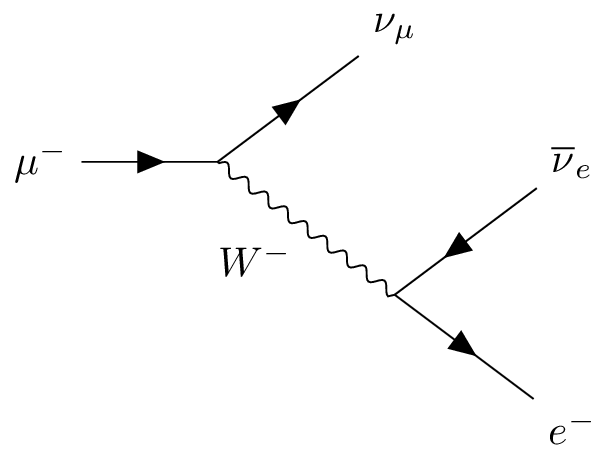
\includegraphics[width=0.4\textwidth]{figures/chapter2/example_feynman_diagram.png}
    \caption{An example feynman diagram describing the $\mu^- \to \nu_\mu \bar{\nu}_e e^-$ decay.}
    \label{fig:example_feynman_diagram}
\end{figure}

%**potentially should add section about propagators**

%**potentially should add a section about renormalization**

\subsection{Scattering}

While correlation functions are the foundational building block of theoretical QFT calculations, it is not immediately obvious with what to do with their result. Physicists think of particles instead of fields (such as in the SM) and are often interested in how they scatter off of one another. These scattering properties allow physicists to compute 
- Cross sections: roughly the rate at which a certain particle is produced.
- Branching fractions: the probability of a specific decay occurring, like is the subject of this thesis. 
which are the two most frequently measured quantities in colliders. So far, correlation functions have only given vacuum expectation values of field operators. 

Formalizing particles in a theory built on fields results in considering particles as eigenstates of the Hamiltonian whose wave packets are non-interacting at either early or late times, called "in" and "out" states respectively. A QFT can thus be equipped with a scattering description only if the Hamiltonian has a complete set of "in" and "out" states. Luckily, the SM is one such QFT.

The scattering properties between these "in" and "out" states can be extracted from the $S$-matrix, or the amplitude to find the world in an "out" state $\beta$, given that it started in an "in" state $\alpha$:
\begin{equation}
S_{\beta \alpha} = \braket{\beta|\alpha}   
\end{equation}
The method of constructing this $S$-matrix from correlation function is done using the LSZ Reduction Formula, which states that the existence of particles in a QFT leads to poles in the Fourier transform of its two-point functions (correlation functions between only two operators, also known as propagators). Therefore, computing the $S$-matrix amounts to computing correlation functions using Feynman Diagrams, taking the Fourier transform, taking all the external momentum to on-shell, and then computing the residue of the pole in the propagator. 

This thesis concerns itself with the branching fraction of the $D^0 \to \mu^+ \mu^-$ interaction. To compute the branching fraction from the scattering amplitude, it is first convenient to remove delta functions and constants always present in the scattering amplitude by defining the $M$-matrix as the matrix that satisfies
\begin{equation}
S_{\beta \alpha} = \delta(\beta -\alpha) + i \times(2\pi)^d \delta^d(p_{\beta}-p_{\alpha}) \mathcal{M}_{\beta \alpha}
\end{equation}
where $p_{\alpha}, p_{\beta}$ are the 4-momentum of the states. 

From this, one can calculate that the differential decay rate into a final state $\beta$ is given by
\begin{equation}
d \Gamma(\alpha \to \beta) = (2\pi)^d \delta^d(p_{\beta}-p_{\alpha}) |\mathcal{M}_{\beta \alpha}|^2 d \beta
\end{equation}
Specifically, to get a full decay width, one must integrate over all final states and their momentum that one cares about to get $\Gamma(\alpha \to \beta) = \int (2\pi)^d \delta^d(p_{\beta}-p_{\alpha}) |\mathcal{M}_{\beta \alpha}|^2 d \beta$. 

This concludes the outline of how to arrive at a branching fraction for a general QFT. The next section covers the specifics of the Standard Model as a QFT and the last section outlines the computation of the $D^0 \to \mu^+ \mu^-$ decay. 

\section{The Standard Model}

Recall that a QFT is constructed by identifying a list of local symmetries and writing down the most general, renormalizable Lagrangian that satisfies the symmetries. The local symmetries of the SM are given by
\begin{equation}
SU(3) \times SU(2) \times U(1)
\end{equation}
Like many QFTs, there are two classifications of fields in the SM: bosons and fermions. While bosons are symmetric under exchange, fermions are antisymmetric under exchange. Consequently, the spin-statistic theorem states that fermions must have half integer spin while bosons have integer spin. Additionally, the spin-statistics theorem dictates that no two fermions may occupy the same state, making it very natural to think of them as matter. The total spin of two interacting half integer spin fermions must be integer, making it natural to think of bosons as mediators of interactions between fermions. 

The three local symmetries of the Standard Model are in fact gauge symmetries. They represent redundancy in the description of our model, similar to the classical electromagnetism gauge. Due to formalism beyond the scope of this thesis, the generators of these gauge groups induce gauge bosons. Specifically, the 8 generators of $SU(3)$ give rise to the eight gluons that describe Quantum Chromodynamics (QCD) and the other four generators of $SU(2) \times U(1)$ give rise to electroweak (EW) interactions. Due to this, it makes sense to break up the Lagrangian into QCD and EW terms, which we know can be written independently, due to the independence of their generators. Namely, we have that
\begin{equation}
\mathcal{L}_{SM} = \mathcal{L}_{EW} + \mathcal{L}_{QCD}
\end{equation}
In the following sections, we will analyze each of these Lagrangians independently, showing how they give rise to the various particles in the SM and their interactions. As a preview, the particles of the Standard Model and their quantum numbers are summarized in figure \ref{fig:particles_of_the_SM}. 

\begin{figure}[ht!]
    \centering
    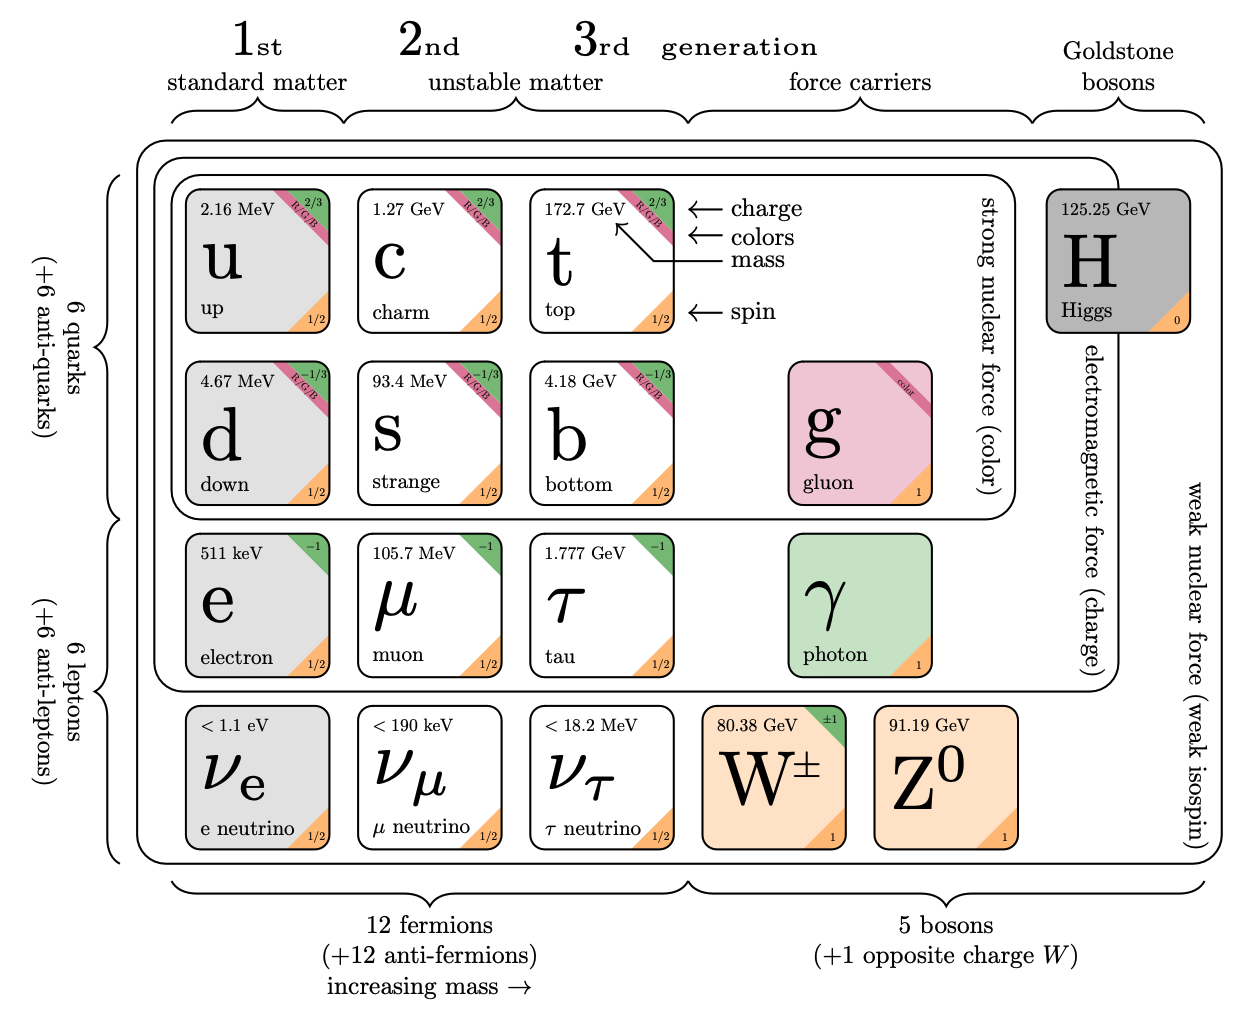
\includegraphics[width=0.8\textwidth]{figures/chapter2/particles_of_the_SM.png}
    \caption{The particles of the Standard Model}
    \label{fig:particles_of_the_SM}
\end{figure}

\subsection{Quantum Chromodynamics}

The eight generators of $SU(3)$ are given by the Gell-Mann matrices and yield the 8 bosons of QCD, known as gluons. The three-dimensional basis of these matrices give rise to three colors, labeled $r$, $g$, and $b$, and three anti-colors, $\bar{r}, \bar{g}, \bar{b}$, which are the fundamental charges of QCD. The Gell-Mann matrices govern that each of the gluons can carry both a color and an anti-color charge. The corresponding fermions in this theory are named quarks and simply carry one color charge or one anti-color charge for anti-quarks. There are 6 different flavors of quarks, summarized in table \ref{tab:quark_masses}. 

\begin{table}[htbp]
    \centering
    \begin{tabular}{@{}lccc@{}}
      \toprule
      Quark & Symbol & Charge $Q/e$ & Mass (MeV/$c^{2}$) \\ 
      \midrule
      Up     & $u$ & $+2/3$ & $2.16^{+0.49}_{-0.26}$ \\
      Down   & $d$ & $-1/3$ & $4.67^{+0.48}_{-0.17}$ \\
      Charm  & $c$ & $+2/3$ & $1270 \pm 20$ \\
      Strange& $s$ & $-1/3$ & $93^{+11}_{-5}$ \\
      Top    & $t$ & $+2/3$ & $172\,760 \pm 300$ \\
      Bottom & $b$ & $-1/3$ & $4180^{+30}_{-20}$ \\
      \bottomrule
    \end{tabular}
    \caption{Electric charge and mass of the six quark flavours.
             Masses are quoted in the schemes recommended by the
             Particle Data Group\,\cite{ref:pdg2024}.}
    \label{tab:quark_masses}
  \end{table}


By constructing a QFT that is invariant under $SU(3)$, one arrives at the Lagrangian
\begin{equation}
    \mathcal{L}_{{QCD}} = \bar{q}^a\cancel{D}_{ab}q^b - m_{ab}\bar{q}^aq^b - \frac{1}{4}G^a_{\mu\nu}G_a^{\mu\nu}
\end{equation}
where $q_i$ is the quark field, with $i$ being the flavor index which is implicitly summed over all the quark flavors. $\cancel{D}$ is a contraction between the gauge covariant derivative and the gamma matrices $\gamma^\mu$ which connect the spinor representation of the fields to the vector representation of the Lorentz group. Stated explicitly, we have
\begin{equation}
    \cancel{D} = \gamma^\mu (D_\mu)_{ab} = \gamma^\mu\left( \partial_\mu \delta_{ab}  - ig_s(G_\mu)_{ab}\right)
\end{equation}
where $G_\mu$ is the gauge field and represented by the Glann-Mann matrices and $g_s$ is the strong coupling constant found in renormalization. $G_{\mu\nu}$ is the associated field strength tensor, given by
\begin{equation}
G_{\mu\nu} = \partial_\mu G_\nu - \partial_\nu G_\mu - ig_s[G_\mu, G_\nu]
\end{equation}
Lastly, $m_{ij}$ resembles the mass matrix of the various quark flavors and is only non-zero when $i=j$.

In general, perturbative calculations in QCD can be quite complex and difficult. Therefore, in practice, QCD is often place on a lattice, imposing a hard momentum cut-off and performing perturbations on the lattice. 

\subsection{Electroweak Interactions}

The electromagnetic and weak nuclear forces are unified under EW interactions at energies above $\approx 250 \text{ GeV}$ or temperatures above $\approx10^{15}$\textdegree $K$, mediated by the $SU(2) \times U(1)$ symmetry. The generators of the $SU(2)$ group yield three gauge bosons of weak isospin, given by $A^i_{\mu}$, and the generators of the $U(1)$ group yield three gauge bosons of weak hypercharge, given by $B_{\mu}$. Importantly, $SU(2)$ is the chiral part of the electroweak symmetry, meaning it only affects left-handed fermions. Therefore, much of the discussion on electroweak interactions will differentiate between left-handed and right-handed particles.

Due to spontaneous symmetry breaking, the four vector bosons are mixed using the Weinberg angle, $\theta_W$, to produce the 4 physical gauge bosons: $\gamma$, $Z^0$, $W^\pm$. Note that the photon, $\gamma$ is sometimes written as the electromagnetic field $A_{\mu}$ and is not to be confused the weak isospin gauge bosons, $A_\mu^i$. Additionally, the $Z^0_{\mu}$ is often just written as $Z_{\mu}$, dropping the charge label. Specifically, the mixing under the Weinberg angle manifests as
\begin{equation}
    \begin{split}
    W^\pm_{\mu} &= \frac{1}{\sqrt{2}}(A^1_{\mu} \mp i A^2_{\mu}) \\
    \begin{pmatrix}
        A_{\mu} \\ Z^0_{\mu}
    \end{pmatrix} &= 
    \begin{pmatrix}
        \cos\theta_W & \sin\theta_W \\
        -\sin\theta_W & \cos\theta_W
    \end{pmatrix}
    \begin{pmatrix}
        B_{\mu} \\ A^3_{\mu}
    \end{pmatrix}
    \label{eq:Weinberg_mixing}
\end{split}
\end{equation}
    

The left-handed fermions in this theory are given as doublets that transform under $SU(2) \times U(1)$ and can be categorized into leptons and quarks. Specifically, the doublet notation is used to manifestly ensure transformation under $SU(2)$. This is similar to a two-state quantum spin system with $\ket{0} = \begin{pmatrix} 1 \\ 0 \end{pmatrix}$ and $\ket{1} = \begin{pmatrix} 0 \\ 1 \end{pmatrix}$ with spin operators that act as $SU(2)$ rotations on the spin vectors. The components of these doublets are the $U(1)$ abiding states, similar to those given by QED interactions.

Therefore, the left-handed leptons are given by
\begin{equation}
L_{i} = \begin{pmatrix}
\nu_{iL} \\ l_{iL}
\end{pmatrix}
\end{equation}
where $\nu_{iL}$ are the three left-handed neutrinos and the $l_{iL}$ particles are the three other left-handed leptons. Notationally, we use $i$ to sum over all three flavors and $L$ to denote the left-handedness of the field. Left-handed quarks are given by
\begin{equation}
Q_{i} = \begin{pmatrix}
u_{iL} \\ V_{ij} d_{jL}
\end{pmatrix}
\end{equation}
where $u_{iL}$ are the three up quarks, $d_{iL}$ are the three down quarks, and $V_{ij}$ is the Cabibbo-Kobayashi-Maskawa (CKM) matrices that keep track of the Weinberg angle mixing coefficients.

The right-handed fermions in this theory are not affected by the $SU(2)$ symmetry; they only transform trivially due to the chirality assigned to the $SU(2)$ symmetry. Therefore, right-handed states are $SU(2)$ singlets that must only abide by $U(1)$ symmetry. We write these to be $u_{iR}$, $d_{iR}$, and $e_{iR}$. However, for notational ease, often the $R$ is dropped since all the left fields are in doublets. Therefore, we write the quark fields as $u_{i}$, $d_{i}$, and $e_{i}$.

\subsubsection{The Higgs field}

Now, there is one more subtlety that must be addressed before introducing the Lagrangian for the electroweak interaction. Specifically, we know that in $d=4$, renormalizable QFTs can only contain non-invariant dimension-four operators, meaning that it cannot allow a term that would give mass to the bosons, such as $m^2 B_{\mu}^aB^{a\mu}$ for the weak isospin gauge bosons.  This is consistent with our formulation of QCD above due to the massless gluon, as well as consistent with our observation of the massless photon. However, the $W^\pm$ and $Z$ boson are observed to carry mass.

Therefore, we must introduce a scalar field that is allowed to break the $SU(2) \times U(1)$ symmetry and give rise to $Z$ and $W^\pm$ masses. This field is known as the Higgs field. While an in-depth discussion of the Higgs mechanism is out of the scope of this thesis, a short discussion should suffice to understand the EW Lagrangian.

In order to give mass to the $W^\pm$ and $Z$ bosons, the field we add must allow for the full Lagrangian to remain invariant while resulting in a ground state that is not. One good way to think of this is known as the Mexican hat potential, given by $f(r, \theta) = (r^2 - v^2)$ shown in figure \ref{fig:Mexican_hat_potential}. This potential is completely rotationally symmetric, but the ground state lies away from the origin at $r = v$, meaning the ground state itself is not spherically symmetric. Additionally it satisfies all other properties of a valid potential by being continuous, well defined, and bounded from below. Therefore, we introduce a doublet under $SU(2)$, given by
\begin{equation}
h = \begin{pmatrix}
h^+ \\ h^0
\end{pmatrix}
\end{equation}
and put it in the Mexican hat potential. 

\begin{figure}[ht!]
    \centering
    \includegraphics[width=0.4\textwidth]{figures/chapter2/Mexican_hat_potential.png}
    \caption{The Mexican hat potential, given by $f(r, \theta) = (r^2 - v^2)$, demonstrating ground state symmetry breaking in a symmetric potential}
    \label{fig:Mexican_hat_potential}
\end{figure}

To see that indeed this gives the $W$ and $Z$ bosons mass, we write down the Lagrangian of this field in the presence of the $W^a_\mu$ and $B_\mu$ fields as
\begin{equation}
\mathcal{L}_{h} = (D_{\mu}h)(D^\mu h) - \lambda\left(|h|^2- \frac{v}{2}\right)^2
\label{eq:higg-field-lagrangian}
\end{equation}
where $D_\mu = (\partial_\mu - \frac{ig}{2}\tau^a A^a_\mu - \frac{ig'Y}{2}B_\mu)$. Here $\tau^a$ (also known as the Pauli matrices) and $YI$ are the generators of $SU(2)$ and $U(1)$. Their corresponding eigenvalues are labeled as $T_a$\footnote{$T_a$ is actually the eigenvalue of $\frac{\tau^a}{2}$} and $Y$; they are known as the weak isospin and weak hypercharge quantum numbers and a convenient basis is often $T^2 = T_1^2 + T_2^2 + T_3^2$, $T_3$, and $Y$. Separately, note that $\lambda\left(|h|^2- \frac{v}{2}\right)^2$ is exactly a rescaled Mexican hat potential. Now, it is straightforward to see that this Lagrangian contains the terms
\begin{equation}
\frac{v^2}{8}\left[g^2\left((A^{1}_{\mu})^2 + (A^{2}_{\mu})^2\right) + (gA_{\mu}^3 - g' B_{\mu})\right]
\end{equation}
giving the intermediate weak isospin and weak hypercharge bosons mass. Using the definition of the Weinberg angle where $\tan(\theta_W) = g'/g$, the mass terms of the observed bosons become
\begin{equation}
M_{W^+} = M_{W^-} = \frac{gv}{2} \quad\quad M_{Z} = \frac{gv}{2\cos(\theta_{W})} \quad\quad M_{\gamma} = 0
\end{equation}

\subsubsection{Full Electroweak Theory}

Finally, by constructing a QFT involving these fields and one that is invariant under $SU(3)$, one arrives at the Lagrangian
\begin{equation}
\mathcal{L}_{EW} = \mathcal{L}_{g} + \mathcal{L}_{f} + \mathcal{L}_{h} + \mathcal{L}_{y}
\end{equation}
where $\mathcal{L}_g$ is the gauge term, similar to the QCD gauge term, given by
\begin{equation}
\mathcal{L}_g = -\frac{1}{4}A^i_{\mu\nu}A^{i\mu\nu} - \frac{1}{4} B_{\mu\nu} B^{\mu\nu}
\end{equation}
The electroweak field strength tensors $A^i_{\mu\nu}$ and $B_{\mu\nu}$ are defined similarly to how the gluon field tensor is defined for QCD.

$\mathcal{L_f}$ is the fermion kinetic term, given by
\begin{equation}
\mathcal{L}_{f} = \bar{L}_{i}\cancel{D}L_{i} + \bar{e}_{i}\cancel{D}e_{i} + \bar{Q}\cancel{D}Q + \bar{u} \cancel{D}u + \bar{d}\cancel{D}d
\label{eq:fermion_kinetic_term}
\end{equation}
where again $\cancel{D}$ is the covariant derivative in the above section, $D_\mu$ contracted with a gamma matrix, $\gamma^\mu$ and the fields are defined in the above section as left-handed doublets and right-handed singlets.

$\mathcal{L}_h$ has already been defined in the previous section and $\mathcal{L}_Y$ are the Yukawa coupling terms between the fermion fields and the Higgs scalar field. This is given by
\begin{equation}
\mathcal{L}_{y} = - Y_{e} \bar{L}he + Y_{u}\bar{Q}h u + Y_{d} \bar{Q}h d
 + \text{h.c.}
\end{equation}
Here, for notational convience we have dropped the flavor indices. $Y_{e,u,d}$ are the three Yukawa coupling term matrices. Just as the Higgs field gives mass to the $W^\pm$ and $Z$ bosons, this mechanism provides mass to the fermions in electroweak theory. 

\section{The $D^0 \to \mu^+ \mu^-$ decay.}

In principle, now that we have written down the SM Lagrangian, one could follow the standard QFT formalism described above to calculate perturbatively $\Gamma(D^0 \to \mu^+ \mu^-)$. In practice, this is incredibly complex and involves decades of perturbative QFT formalisms. Therefore, in this section we will first categorize this decay as a FCNC and briefly summarize the heuristic structure of the calculation of $\mathcal{B}(D^0 \to \mu^+ \mu^-)$ as performed by G. Burdman, E. Golowich, J. L. Hewett, and S. Pakvasa (BGHP) \cite{ref:burdman_2002}.

\subsection{Flavor Changing Neutral Currents}

Flavor changing neutral currents (FCNCs) are interactions that change the flavor of a fermion without altering its electric charge. 

The SM forbids FCNCs explicitly at tree level. Processes that are flavor-changing with neutral currents must occur through loop processes that result in a neutral current, the details of which are discussed later. To illustrate this explicitly, we start with the gluon-fermion interaction terms of the Lagrangian which we derived earlier. Namely we have that the interaction terms can be pulled out of equation \ref{eq:fermion_kinetic_term} to give us
\begin{equation}
\mathcal{L}_{gf} = \sum_{f=\{ Q, L, u, d, e\}} \bar{f}_{i} \gamma^\mu \left(\partial_\mu - \frac{ig}{2} \tau^a A^a_\mu - ig' \frac{Y}{2} B_\mu\right)f_{i}
\end{equation}
We now rotate into the Weinberg basis, using $\tau^\pm = \frac{\tau^1 \pm i\tau^2}{\sqrt{2}}$ and $W^\pm$ defined as in equation \ref{eq:Weinberg_mixing}. This gives us
\begin{equation}
\mathcal{L}_{gf} = \sum_{f=\{ Q, L, u, d, e\}} \bar{f}_{i} \gamma^\mu \left(\partial_\mu - \frac{ig}{\sqrt{2}} (W^+_\mu\tau^+ + W_\mu^- \tau^-) -\frac{g}{2} A^3_\mu\tau^3 - \frac{g'}{2}B_\mu Y\right)f_{i}
\end{equation}
From this, we can easily isolate $\mathcal{L}_{gf}$ into neutral currents and charged currents, as $\tau^\pm$ is the charged operator.\footnote{This fact is not explicitly proven here, but can be shown by writing out $\tau^\pm$ in the doublet basis and then noticing that $\tau^+$ converts the lower component into the upper one while $\tau^-$ does the opposite. This causes the weak isospin eigenvalue to change while keeping hypercharge constant, resulting a change in electric charge, $Q = I_3 + Y/2$} Therefore, we have that the neutral current interactions are given by
\begin{equation}
\mathcal{L}_{NC} = \sum_{f=\{ Q, L, u, d, e\}} \bar{f}_{i} \gamma^\mu \left( -\frac{g}{2} A^3_\mu\tau^3 - \frac{g'}{2}B_\mu Y\right)f_{i}
\end{equation}
Now, we notice that the Lagrangian only has interactions between fermions with the same flavor index. Therefore, the only flavor mixing that can occur is between the doublets. Therefore, we can expand out to get the candidates for FCNC interactions as
\begin{equation}
\begin{split}
\mathcal{L}_{\text{FCNC Candidates}} = &-\frac{g}{2}\begin{pmatrix}
\bar{u}_{iL} & \bar{d_{iL}}
\end{pmatrix} \gamma^\mu A_{\mu}^3 \begin{pmatrix}
1 & 0 \\ 0 & -1
\end{pmatrix} \begin{pmatrix}
u_{iL} \\ d_{iL}
\end{pmatrix} \\
&-\frac{g}{2}\begin{pmatrix}
\bar{\nu}_{iL} & \bar{l_{iL}}
\end{pmatrix} \gamma^\mu A_{\mu}^3 \begin{pmatrix}
1 & 0 \\ 0 & -1
\end{pmatrix} \begin{pmatrix}
\nu_{iL} \\ l_{iL}
\end{pmatrix} \\
&-\frac{g'}{2}\begin{pmatrix}
\bar{u}_{iL} & \bar{d_{iL}}
\end{pmatrix} \gamma^\mu B_{\mu} \begin{pmatrix}
1 & 0 \\ 0 & 1
\end{pmatrix} \begin{pmatrix}
u_{iL} \\ d_{iL}
\end{pmatrix} \\
&-\frac{g'}{2}\begin{pmatrix}
\bar{\nu}_{iL} & \bar{l_{iL}}
\end{pmatrix} \gamma^\mu B_{\mu} \begin{pmatrix}
1 & 0 \\ 0 & 1
\end{pmatrix} \begin{pmatrix}
\nu_{iL} \\ l_{iL}
\end{pmatrix}
\label{eq:large-eq-for-FCNC-candidates}
\end{split}
\end{equation}
Now, we can consolidate this significantly by introducing $e = g\sin(\theta_W) = g'\cos(\theta_W)$\footnote{The second equality can be verified by using $\tan(\theta_W) = \frac{g'}{g}$}, $A^3_\mu = \cos(\theta_W)Z_\mu + \sin(\theta_W)A_\mu$, and $B_\mu = -\sin(\theta_W)Z_\mu + \cos(\theta_W) A_\mu$. The second two equations can be derived from equation \ref{eq:Weinberg_mixing}. Additionally, we can use the weak isospin and weak hypercharge eigenvalues $I_3$ and $Y$, defined below equation \ref{eq:higg-field-lagrangian}.  It is also useful to define the electric charge eigenvalue, $Q = I_3 + Y/2$. Using this, we can greatly simplify equation \ref{eq:large-eq-for-FCNC-candidates} to
\begin{equation}
\begin{split}
\mathcal{L}_{\text{FCNC Candidates}} &= -\sum_{f = u_{L},d_{L},l_{L}, \nu_{L}} \left[\frac{e}{\sin(\theta_{W})\cos(\theta_{W})} \bar{f}_{i}\gamma^\mu Z_{\mu}\left(T_{3}^{(f)} -Q^{(f)}\sin^2(\theta_{W})\right)\bar{f}_{i}\right]\\
&- \sum_{f = u_{L},d_{L},l_{L}, \nu_{L}} \left[ e \bar{f}_{i}\gamma^\mu A_{\mu}Q^{(f)}f_{i}\right]
\end{split}
\end{equation}
where the values of $T_3^{(f)}$, $Y^{(f)}$ and $Q^{(f)}$ can be found in table \ref{tab:ew_charges}. 


\begin{table}[htbp]
    \centering
    \begin{tabular}{|lccc|lccc|}
      \hline
      \multicolumn{4}{|c|}{\textbf{Left‑handed fermions}} &
      \multicolumn{4}{c|}{\textbf{Right‑handed fermions}} \\
      \hline
      Field & $T_3$ & $Y$ & $Q/e$ &
      Field & $T_3$ & $Y$ & $Q/e$ \\
      \hline
      Up quark $u_L$        & $+1/2$ & $+1/3$ & $+2/3$ &
      Up quark $u_R$        & $0$    & $+4/3$ & $+2/3$ \\
      Down quark $d_L$      & $-1/2$ & $+1/3$ & $-1/3$ &
      Down quark $d_R$      & $0$    & $-2/3$ & $-1/3$ \\
      Neutrino $\nu_L$      & $+1/2$ & $-1$   & $0$    &
      Charged lepton $l_R$  & $0$    & $-2$   & $-1$   \\
      Charged lepton $l_L$  & $-1/2$ & $-1$   & $-1$   &
                            &        &        &        \\
      \hline
    \end{tabular}
    \caption{Weak isospin $(T_3)$, weak hypercharge $(Y)$, and electric
             charge $(Q)$ for the chiral fermions of one Standard Model
             generation\,\cite{ref:pdg2024}.}
    \label{tab:ew_charges}
  \end{table}
  
  

More importantly, we confirm that no flavor-changing neutral current terms remain at tree level in the SM. More specifically, there are no terms that allow for interactions between fermions of two different flavors. Therefore, we have that $\mathcal{L}_{FCNC} = 0$ under the SM, preventing FCNC at tree level. 

\subsection{The $D^0 \to \mu^+ \mu^-$ decay as a FCNC}

Hadrons, such as the $D^0$ are collections of quarks in bound states. One defining property of QCD is that virtually all hadrons are in gluon-bound color-neutral states. These states therefore contain either a quark triplet (known as baryons) or a quark and an antiquark (known as mesons). $D$ mesons are known as charm mesons and are any light meson that contains a charm quark. The $D^0$ is one such meson, being the only neutral $D$ meson, composed of a charm and an anti-up quark. Note that there is also an anti-$D^0$ meson, being composed of an anti-charm and an up quark. 

Now, since the $D^0$ meson is composed of a quark pair and the final state $\mu^+ \mu^-$ contains no quarks, therefore implying a flavor change. However, importantly the $D^0$ is a neutral particle, as is the $\mu^+ \mu^-$ final state. Therefore, for there to be a tree-level contribution, there must be a tree-level FCNC, which is not allowed by the Standard Model. Therefore, the $D^0 \to \mu^+ \mu^-$  must proceed via higher-order loop processes, resulting in strong suppression in the SM.

G. Burdman, E. Golowich, J. L. Hewett, and S. Pakvasa (BGHP) have carried out the most complete SM analysis of the $D^0 \to \mu^+ \mu^-$ decay that includes all short and long-distance effects. 

To begin with the short distance (SD) effects, the quark level transition arises from electroweak penguin and box diagrams, an example of which is found in Feynman diagram in figure \ref{fig:D0_decay_diagrams}. After integrating over all possible diagrams, BGHP find that 
\begin{equation}
\mathcal{B}(D^0 \to \mu^+ \mu^-)_{SD} \simeq 10^{-18}
\end{equation}

\begin{figure}[ht!]
    \centering
    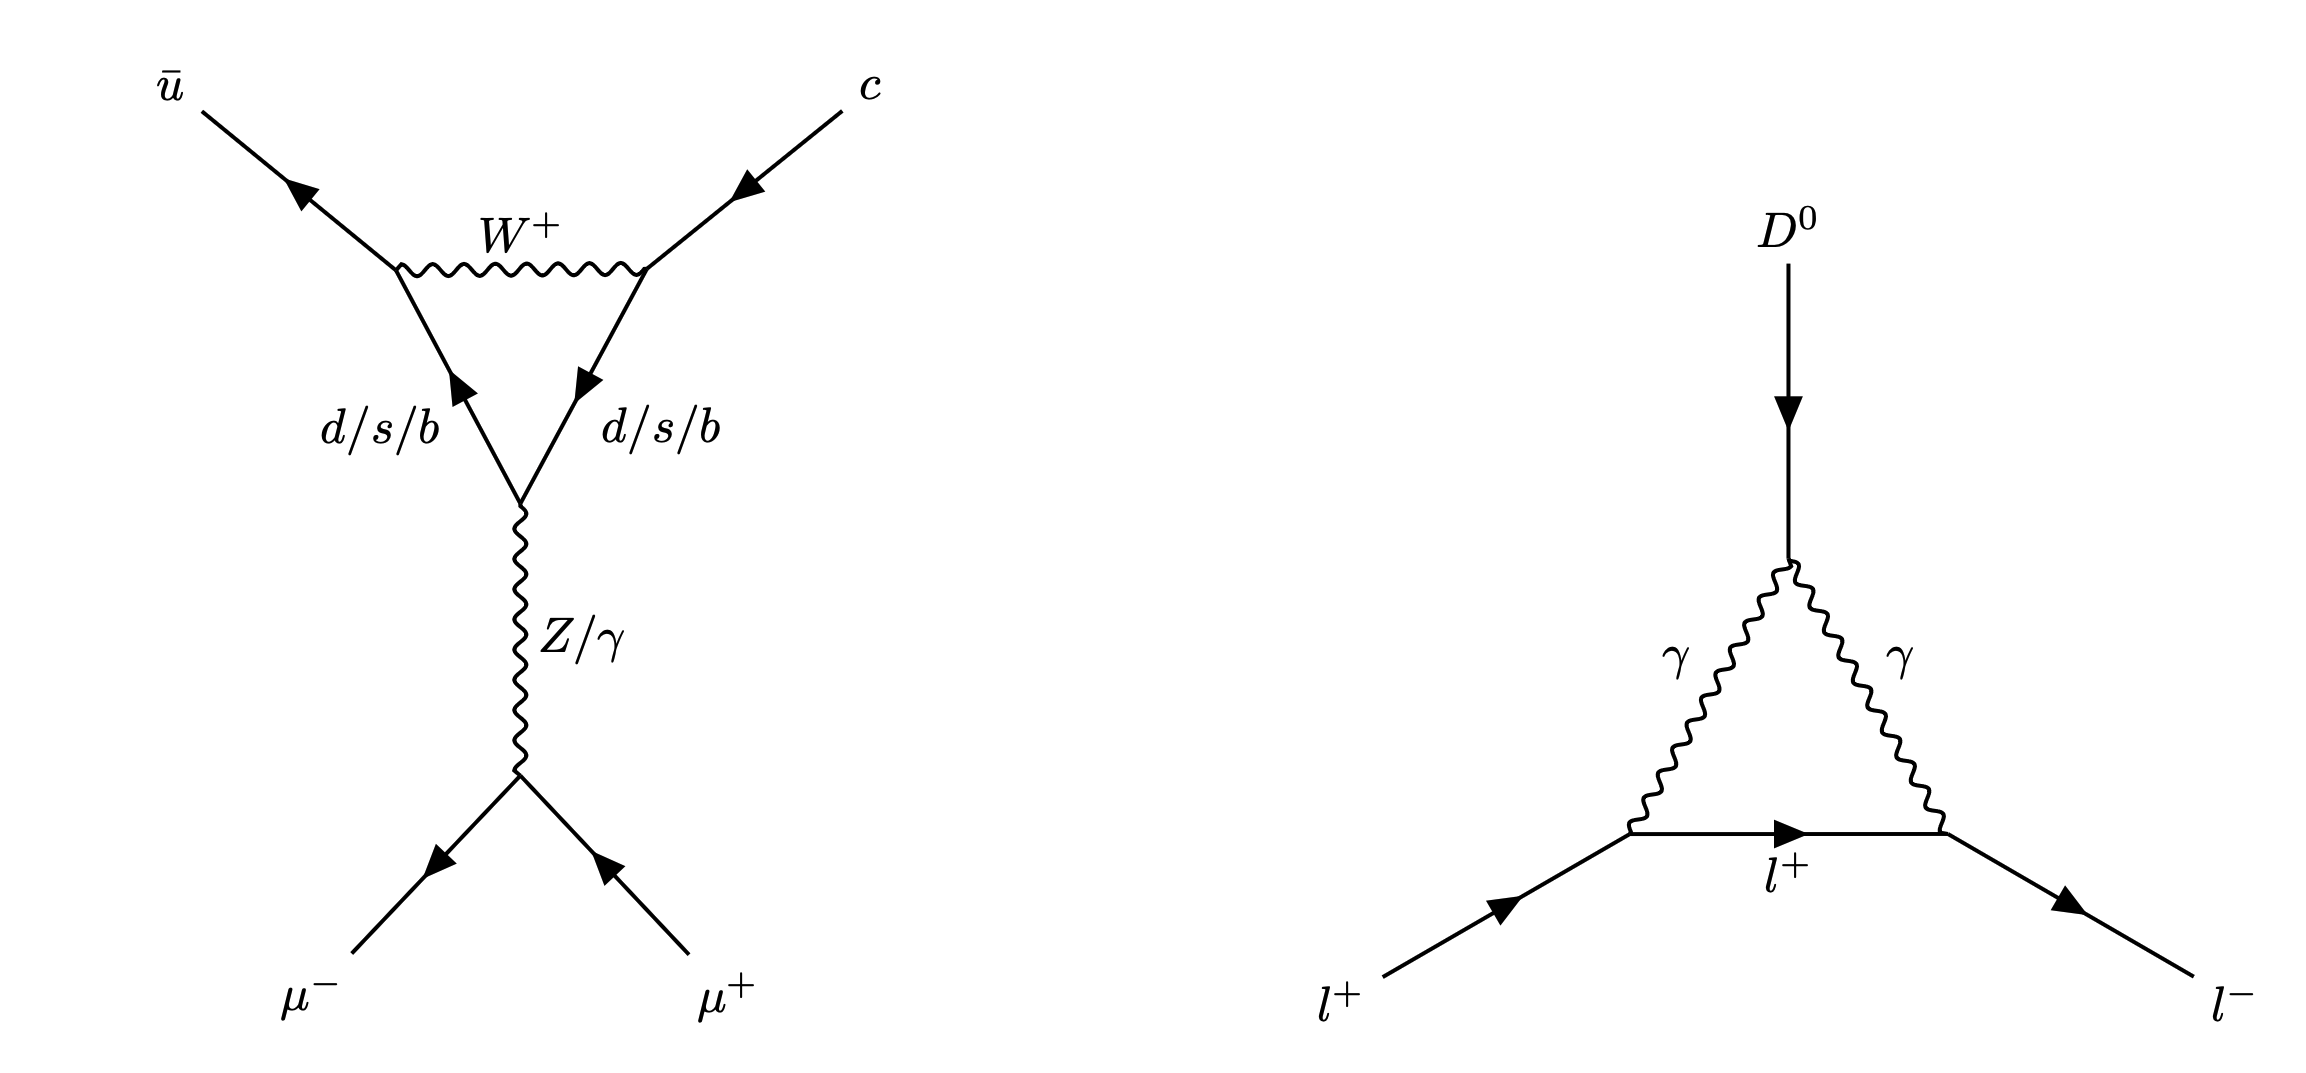
\includegraphics[width=1.0\textwidth]{figures/chapter2/d0_FCNC_decays.png}
    \caption{Two Feynman diagrams contributing to rare \(D^0\) decays: (left) the leading SD contribution in the form of a penguin diagram and (right) the leading LD contribution, depicting the two-photon contribution. Note that the $D^0$/$\gamma$/$\gamma$ vertex hides additional complexity in the Feynman diagram, which is calculated by BGHP in the form of many SD and LD contributions combined and is abstracted away in the above diagrams.}
  \label{fig:D0_decay_diagrams}
\end{figure}

Next, BGHP identify two distinct long distance (LD) mechanisms, single-particle unitary contributions and two-photon contributions. The single particle unitary contributions are dominated by weak-mixing with ground-state presudoscalars, such as $\pi^0, \eta, \eta'$, followed by these pseudoscalars decaying into a dimuon final state, $P^0 \to \mu^+ \mu^-$. The branching fraction of this calculation is given by
\begin{equation}
\mathcal{B}(D^0 \to \mu^+ \mu^-)_{\pi^0, \eta, \eta'} \simeq 2.5 \times 10^{-18}
\end{equation}
In principle, there could be mixing with heavier $0^\pm$ resonances such as $\pi(1800)$; however, the decays of $\pi(1800) \to \mu^+\mu^-$ occur with a branching fraction likely around $10^{-12}$, leading to
\begin{equation}
\mathcal{B}(D^0 \to \mu^+ \mu^-)_{\pi(1800)} \simeq  5.0 \times 10^{-17}
\end{equation}
The two-photon contributions come from the dispersive two photon decay $D^0 \to \gamma \gamma \to \mu^+ \mu^-$ shown in figure \ref{fig:D0_decay_diagrams}. BGHP show that 
\begin{equation}
\mathcal{B}(D^0 \to \mu^+ \mu^-)_{\gamma\gamma} \simeq 2.7 \times 10^{-5} \mathcal{B}(D^0 \to \gamma\gamma)
\end{equation}
where their own calculations show that, by considering short distance contributions, long distance vector meson dominant contributions, long distance single particle unitary contributions, and long distance two-particle unitary contributions, $\mathcal{B}(D^0 \to \gamma\gamma) \simeq 10^{-8}$. Therefore, 
\begin{equation}
\mathcal{B}(D^0 \to \mu^+ \mu^-)_{\gamma\gamma} \simeq 10^{-13}
\end{equation}
When summing each of these contributions, one finds that $\mathcal{B}(D^0 \to \mu^+ \mu^-)_{\gamma\gamma} \simeq 10^{-13}$ is by far the dominant contribution to the total branching fraction, therefore BGHP conclude that
\begin{equation}
\mathcal{B}(D^0 \to \mu^+ \mu^-)_{\text{total}} \simeq 10^{-13}
\end{equation}
It is also worth noting that BGHP show that various new physics models significantly increase this branching fraction. However, their work on this is far out of the scope of this thesis and outlines many different new physics models, including many commonly accepted candidates for Beyond the Standard Model (BSM) physics such as Flavor Non-Universal Z' Bosons and Super Symmetry (SUSY). One such model is Flavor Non-Universal Z' Bosons, which introduce neutral Z' bosons with flavor off diagonal couplings 

Due to the complexity and number of these models, we simply refer to their work to give meaningful calculations in support of new physics should a branching fraction significantly larger than $10^{-13}$ be detected. It should be clear from these calculations that putting better limits on $\mathcal{B}(D^0 \to \mu^+ \mu^-)$ acts as a meaningful probe into many new physics models, serving as the primary motivation of this work. 
\chapter{The CMS Detector}
\label{ch:3}

This chapter describes the experimental framework underlying the measurement of the $D^0 \to \mu^+ \mu^-$ branching fraction. It begins with a summary of the Large Hadron Collider at CERN, covering the injector chain, magnet systems, running periods, and luminosity profile. 

Then, this chapter describes the CMS detector beginning with a short overview of its geometry and coordinate system before diving into each of its subsystems, including the silicon tracker, electromagnetic calorimeter, hadronic calorimeter, superconducting solenoid, and muon chambers. For each of the subsystems, this chapter describes both the basic engineering needed for these detectors and the effect on the physics read-out from the detector. 

Lastly, this chapter describes how the CMS experiment uses a trigger system to balance the large volume of data with the need to capture sufficient numbers of rare particle interactions. 

\section{The Large Hadron Collider}

The Large Hadron Collider (LHC) at the European Organization for Nuclear Research (CERN) is one of the largest experiments in the world. It has a circumference of 26.7 km, spanning the border of Switzerland and France near Geneva, Switzerland. As the name might suggest, the LHC is a two-ring superconducting hadron accelerator focusing on proton-proton collisions with occasional heavy-ion collision runs. For this thesis, we will entirely focus on proton-proton collisions.

The protons originate from hydrogen atoms, from which electrons are stripped using a strong electric field to isolate the protons. From there, a series of accelerators called the CERN LHC injector chain accelerates the protons to 450 GeV before injecting them into the LHC in bunches. At any given time, there are 39 batches of 72 proton bunches in the LHC with a 25 ns bunch spacing to accommodate the LHC kicker's rise time.

Once injected, the proton bunches are accelerated to a center-of-mass energy of several TeV using two main types of magnets: (i) 1,232 dipole magnets with a field strength of 8.3 T, which bend and accelerate the protons along the circular beam pipes, and (ii) 492 superconducting quadrupole magnets, operated at 1.9 K, which focus the proton bunches to maintain beam stability.

Once the particles are accelerated to their target energy, they collide at four main interaction points within the LHC. These correspond to the four major LHC experiments: two general-purpose detectors capable of a broad range of physics analysis: ATLAS (A Toroidal LHC Apparatus) and CMS (Compact Muon Solenoid); one detector optimized for heavy-ion collisions: ALICE (A Large Ion Collider Experiment); and one detector focused on $b$-physics: LHCb. In addition, five smaller experiments are located at secondary sites in the LHC: two specialized in forward-scattered particles, one experiment near LHCb to look for magnetic monopoles, and two experiments near ATLAS specialized in light particles, such as neutrinos. The full CERN accelerator complex can be seen in Figure \ref{fig:cern-accelerator-complex}

\begin{figure}[htbp]
    \centering
    \includegraphics[width=0.8\textwidth]{figures/chapter3/CERN-accelerator-complex.png}
    \caption{The CERN accelerator complex \cite{ref:Lopienska}}
    \label{fig:cern-accelerator-complex}
\end{figure}


One of the main difficulties of circular colliders is the rapid energy loss of every through synchrotron radiation, the electromagnetic radiation emitted when relativistic charged particles move along a curved path. The total power radiated by synchrotron radiation in circular colliders is given by
\begin{equation}
    P = \frac{q^2p^4}{6 \pi \epsilon_0 m^4 c^5 r^2}
\end{equation}
where $q$ is the charge of the particles, $p$ is the momentum of the particle, $m$ is the rest mass of the particle, and $r$ is the radius of the collider. This provides the LHC with two key advantages in minimizing synchrotron radiation losses while achieving high beam energies: (i) compared to electron-positron colliders, such as the LHC's predecessor the Large Electron-Positron collider, the mass of protons is much larger and (ii) the radius of the LHC is larger than any other collider in the world. 

Another difficulty of high energy colliders is the rarity of physically interesting collisions. Not only is it difficult to have two protons collide, but it is also rare to have a collision that will get included in an analysis. Due to these factors, the LHC operates at a very high beam intensity, measured by its luminosity. The luminosity of an accelerator is given by
\begin{equation}
    L = \frac{N_b^2n_b f_{rev} \gamma_r F}{4 \pi \epsilon_n \beta^*}
\label{eq:luminosity}
\end{equation}
where $N_b$ is the number of protons per bunch, $n_b$ is the number of bunches per beam, $f_{rev}$ is the revolution frequency, $\gamma_r$ is the Lorentz factor, $F$ a geometric factor, and lastly $\epsilon_n$ and $\beta^*$ determine the interaction rate at the interaction point. The high luminosity at the LHC is achieved largely with the $\approx 10^{11}$ protons per bunch. However, this high intensity introduces numerous challenges due to the high number of background collisions, which we will discuss further in Section \ref{sec:triggers}.

Instead of running continuously, the LHC breaks up its data collecting into runs, each at a different center-of-mass energy and luminosity. The first run from 2010-2012 had a 8 TeV center-of-mass energy with a total luminosity of $29.45 \; \text{fb}^{-1}$. Run 2 occurred from 2015-2018 and had a 13 TeV center-of-mass energy with a total luminosity of $163.6 \; \text{fb}^{-1}$. Run 3 started in 2022 and is currently ongoing with a center-of-mass energy at $13.6$ TeV and a targeted luminosity of $42 \; \text{fb}^{-1}$. 

\section{The CMS Detector}

The CMS detector is a large cylindrical detector that almost entirely wraps around the proton beam. It is 21 meters long and 15 meters in diameter, weighing 14,000 tonnes. It is composed of 5 main subsystems wrapped in layers around the beam pipe. These five layers are the silicon tracker, the electromagnetic calorimeter, the hadron calorimeter, and the superconducting solenoid, and the muon chambers. These layers are wrapped around the beam line through the center of the detector and can be seen in Figure \ref{fig:cms-detector-cutout.png}. More discussion on the subsystems of CMS will proceed in following sections. However, one must first understand the coordinate system.

\begin{figure}[htbp]
    \centering
    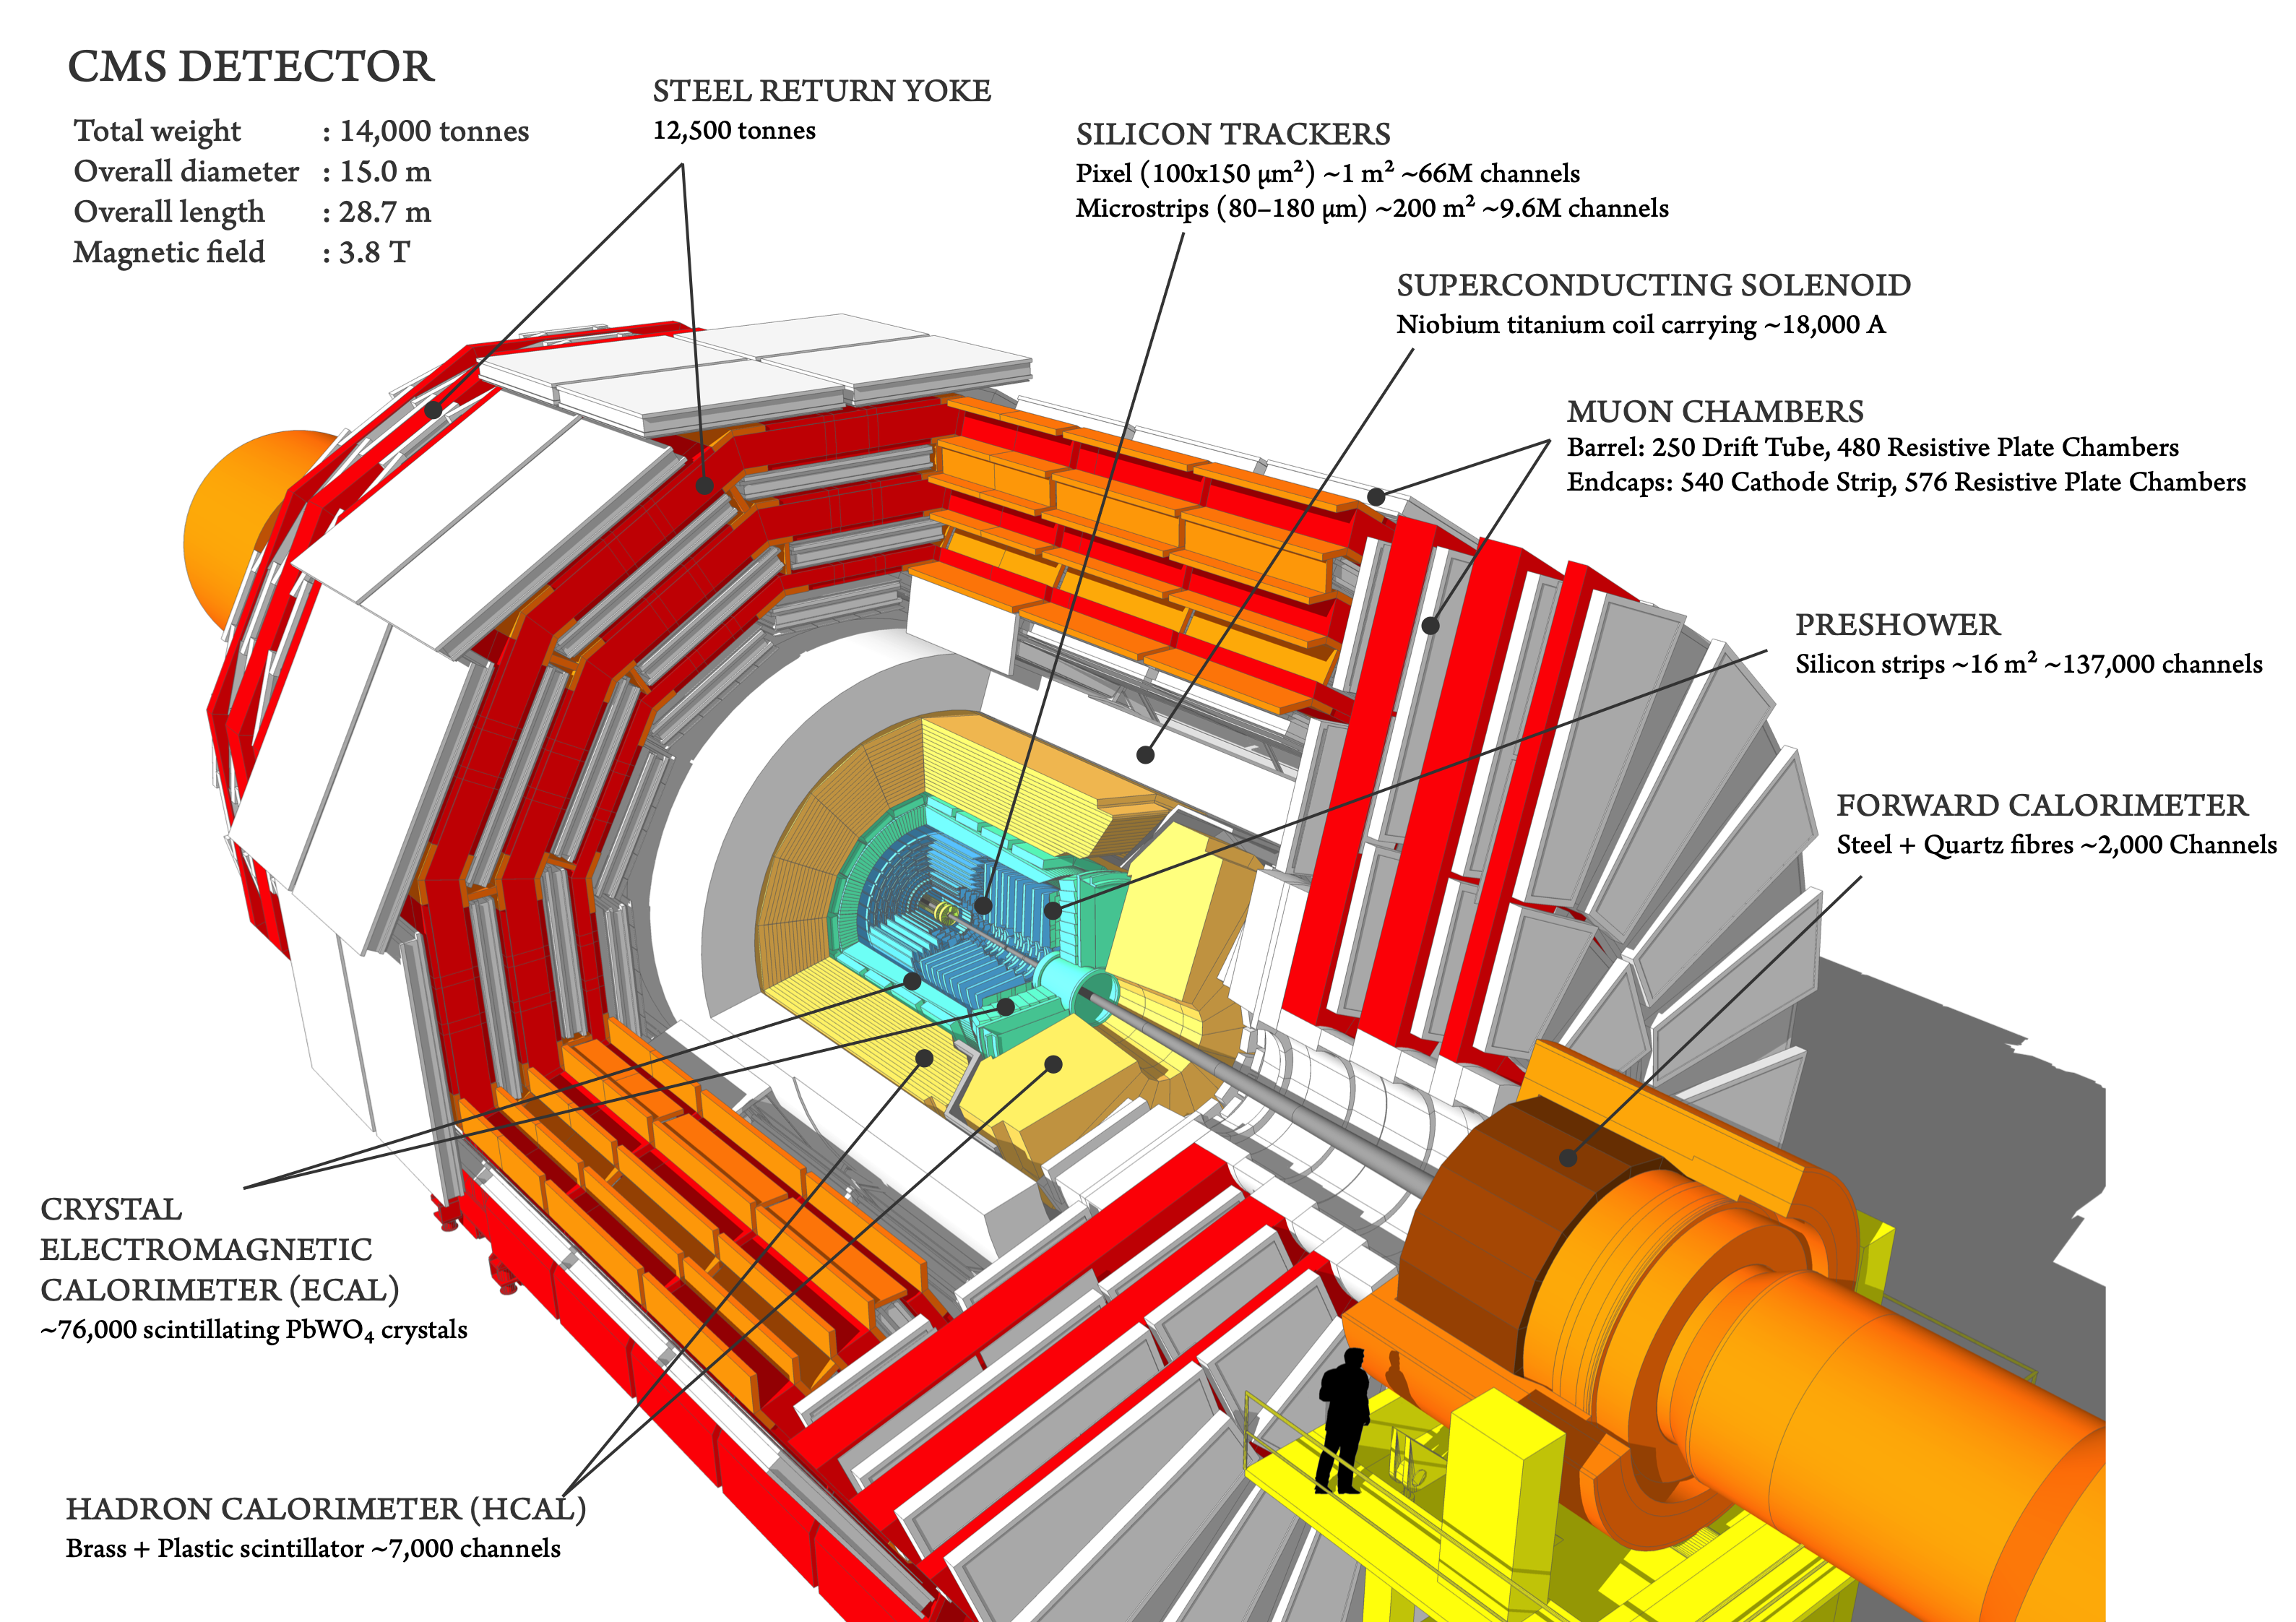
\includegraphics[width=0.8\textwidth]{figures/chapter3/cms-detector-cutout.png}
    \caption{A labeled cutaway diagram of the CMS detector \cite{ref:sakuma}}
    \label{fig:cms-detector-cutout.png}
\end{figure}


The coordinates used in CMS are $\phi, \eta,$ and $r$ with the origin located at the interaction vertex at the center of the cylinder where $r$ represents the distance from the point of interest to the origin. $\phi$ describes the azimuthal angle along the plane normal to the beam line and is often ignored due to the complete symmetry in $\phi$. Lastly, $\eta$ is known as the pseudorapidity, describing the angle of a particle relative to the beam line, $\theta$, as
\begin{equation}
    \eta \equiv -\ln\left[ \tan(\left(\frac{\theta}{2}\right) \right]
\end{equation}
For high energy particles, this is a good approximation of rapidity, given by
\begin{equation}
    y = \frac{1}{2} \ln\left( \frac{E + p_z}{E-p_z}\right)
\end{equation}
where $p_z$ is the momentum along the beam line. This is used instead of the conventional angle $\theta$ because rapidity is invariant under Lorentz boosts while the standard angle $\theta$ is not. For example, if two particles have rapidities $y_1$ and $y_2$ and the difference $y_1 - y_2$ is invariant in any reference frame. The CMS detector has two main regions: the barrel which wraps around the beam pipe and the endcaps which cover the ends of the cylinder. The exact $\eta$ value separating the barrel and endcap regions varies by subsystem at CMS, but needs to be carefully considered due to biases introduced because of detector geometry as you move from the barrel to the endcap. 

One other quantity frequently used in describing particle kinematics is $p_T$, or the momentum of the particle transverse to the beam line given by
\begin{equation}
    p_T = |\vec{p}|\text{sech}(\eta)
\end{equation}
The full set of coordinates and the CMS geometry can be seen in Figure \ref{fig:cms-coordinate-system}.

\begin{figure}[hb!]
    \centering
    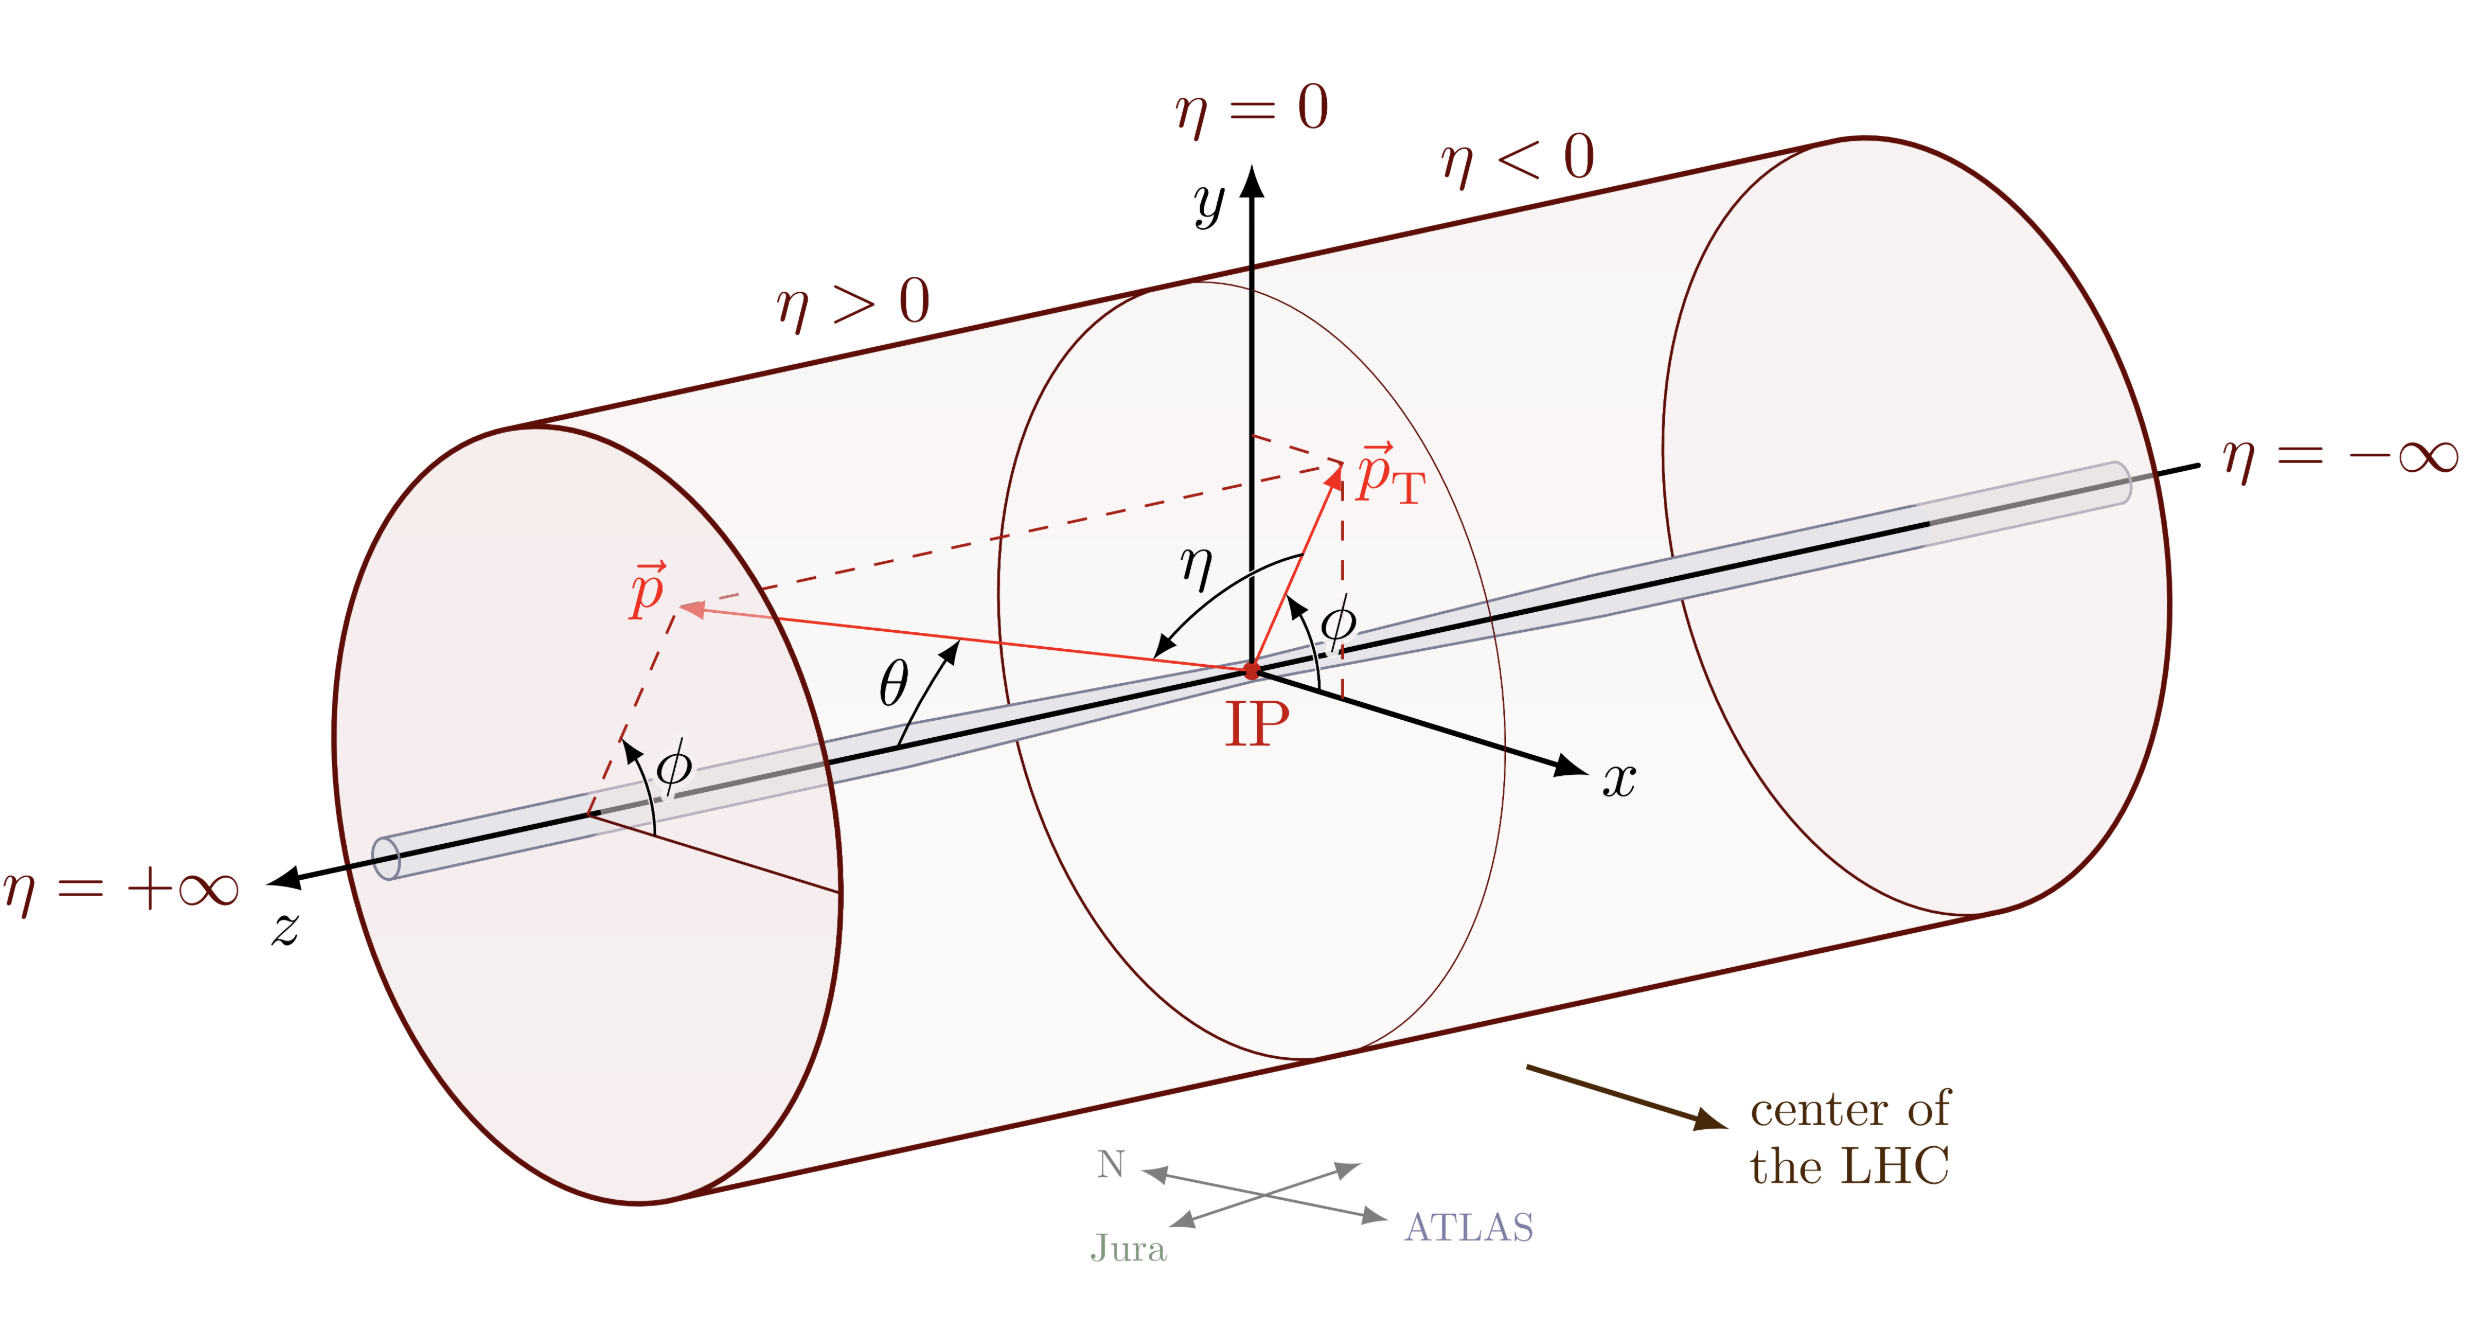
\includegraphics[width=1.0\textwidth]{figures/chapter3/CMS-coordinate-system.png}
    \caption{The CERN accelerator complex}
    \label{fig:cms-coordinate-system}
\end{figure}



\subsection{Solenoid Magnet}

One of the easiest ways to measure the electromagnetic charge of high energy particles is to introduce them into a strong magnetic field and measure the curvature of their tracks. Additionally, the curvature is also dependent on the momentum of the incoming particle, allowing the detector to reconstruct the momentum of charged particles from their tracks. Therefore, the presence of a strong magnetic field across all other subsystem is essential. 

The CMS detector contains a 3.8 T solenoid magnet in the middle of the other subsystems. The solenoid is approximately 6 meters in diameter and 13 meters in length, making it one of the largest of its kind ever constructed. Its immense field strength enables CMS to accurately reconstruct the trajectories and momenta of particles produced in collisions, even at very high energies.

\subsection{Silicon Tracker}

Before the tracks of particles can be disturbed by interactions with other detector components, the silicon tracker reconstructs a precise track that records the particle's trajectory. This is most commonly used for locating their primary vertices, the exact location of their production, as well as assisting in kinematic reconstruction. In order to do this, silicon is configured in a reverse-biased p-n junction. As charged particle pass through the silicon, they ionize silicon atoms, creating electron-hole pairs. This electric field pushes electrons toward the n-type electrode and hole toward the p-type electrode, causing a current pulse. This current pulse is then read out by Application-Specific Integrated Circuits (ASICs). Because this detection relies on ionization, neutral particles do not produce signals in the tracker.

The detector is made of two layers of silicon detectors: small pixels located near the center of the tracker and larger strips located near the outside of the detector. The pixels have a size of $100 \times 150 \mu m$, allowing for them to have an extremely fine resolution. Further out, the large strips arranged in a vertical/horizontal pattern reconstruct the track of charged particles by superimposing the vertical and horizontal signals. This allows for more precise modeling of the particle's position, but at the cost of resolution. Strips closer to the center of the detector are smaller while strips further outside are larger. 

\subsection{Electromagnetic Calorimeter}
A calorimeter is any device that measures the heat exchanged between a process and its environment.  In particle physics detectors, the term takes on a specialized meaning: it denotes a system that destructively measures a particle's energy by scattering it in dense material and recording the ensuing shower.  Such devices therefore contain two essential components: (i) a passive absorber, which initiates the shower, and (ii) a scintillating medium, which converts the energy released by the shower into optical photons that can be read out.

Perhaps the most common example of a calorimeters is the electromagnetic calorimeter (ECAL), whose purpose is to stop and measure high-energy electrons and photons.  Incoming $\gamma/e^{\pm}$ particles lose energy almost exclusively through well-understood QED processes such as bremsstrahlung and pair production, causing a cascade to lower energy photons and electrons, causing an electromagnetic shower such as in Figure \ref{fig:electromagnetic-shower}. Eventually the cascaded photons and electrons have a low enough energy that they are able to be easily absorbed and measured by the scintillator.  The characteristic scale of this shower is the radiation length~$X_{0}$, the mean distance over which an electron's energy is reduced by a factor~$e^{-1}$.  In practice an ECAL is built to a depth of $\sim\!20$-30\,$X_{0}$ so that the entire shower is contained. The other important scale is the Molière radius, or the radius of the cylinder containing $90\%$ of the shower's energy.

\begin{figure}[htbp]
    \centering
    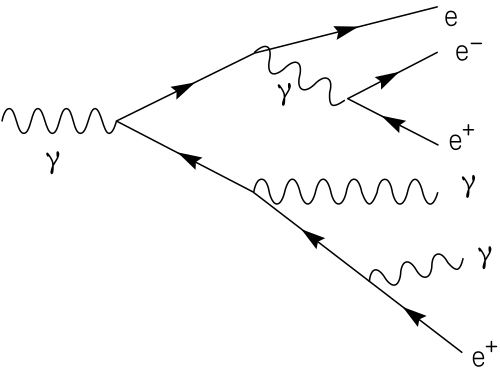
\includegraphics[width=0.4\textwidth]{figures/chapter3/electromagnetic-shower.png}
    \caption{A schematic example of an electromagnetic shower caused by bremmstrahlung and pair production.}
    \label{fig:electromagnetic-shower}
\end{figure}

In CMS the ECAL is a homogeneous calorimeter, meaning the absorber and the scintillator are the same material (lead tungstate, PbWO$_4$) so that virtually no energy is lost to passive absorbers since they are the same as the scintillator. Additionally, homogeneous calorimeters allow for the same response from every angle due to their homogeneity. The barrel section ($|\eta|<1.48$) and two end-caps ($1.48<|\eta|<3.0$) together comprise 75,848 crystals, each $22\times22\;\text{mm}^2$ at the front face and $230\;\text{mm}$ long ($25.8\,X_{0}$). The fast scintillation time of PbWO$_4$ ensures that $\sim80\%$ of the light is collected within a single LHC bunch crossing, and the small Molière radius ($R_M\simeq21$ mm) localizes showers largely inside one crystal.  

Radiation damage gradually darkens the crystals. Therefore, CMS injects laser light between fills to monitor transparency and applies time-dependent calibration constants. This careful calibration allows for precise reconstruction of an electromagnetic particle's energy. 


\subsection{Hadronic Calorimeter}
While the ECAL measures purely electromagnetic showers, the hadronic calorimeter (HCAL) captures and quantifies the energy of neutral and charged hadrons.  The underlying physics is much more complex. When an incoming hadron interacts strongly with the passive absorber of the HCAL, it produces a hadron shower. The hadrons in the shower then produce electrons and photons in three main ways: (i) through neutral pions which decay to charged kaons or protons, which interact to produce two photons through athreevertex feynman diagram, (ii) through charged hadrons ionizing the passive absorber, and (iii) through evaporation and spallation of the nuclei of the passive absorber. Then, these photons and electrons produce showers which are measured, similar to the ECAL. While neutral pion decay accounts for most of the energy converted to electromagnetic showers, the specific fraction of hadron energy that is converted to photon/electron energy is highly dependent on the incoming hadron's momentum and energy. This leads to a lower energy resolution compared to ECALs since it is difficult to estimate how much energy is not converted to photons and electrons. Additionally, because of the addition of hadron showers in HCALs, the radiation length of the HCAL is longer, leading to a larger detector compared to ECALs. 


CMS uses a sampling HCAL.  Alternating layers of passive brass absorber and plastic scintillator tiles form a barrel ($|\eta|<1.3$), two end-caps ($1.3<|\eta|<3.0$), and a forward calorimeter extending to $|\eta| < 5.2$. Radiation and aging also affect HCAL response, similar to ECALs. CMS calibrates the system continuously using embedded radioactive sources, dedicated laser/LED pulses, and $\phi$-symmetry methods.

\subsection{Muon Chambers}

Lepton detection is critical to many anylses performed at CMS, including this one, which focuses on muon and electron final states. Neutrinos are too light to be detected by anything in the detector and $\tau$ leptons are so unstable they always decay into other products which we measure. Electrons are well measured in the ECAL, but muons are heavy enough that they almost always don't get absorbed by the ECAL and therefore are not detected. Therefore, there is a need to construct large muon chambers, specifically built to detect muons. 

The muon chambers work by measuring the muon's track as it leaves the detector. The magnetic field is still strong enough that the momentum  and sign of the charge of the muon can directly be reconstructed from the curvature of the track. In this way, the muon chambers can be thought of as very large trackers. 

There are three different types of gaseous detectors used in the muon system: drift tubes, cathode strip chambers, and resistive plate chambers. The drift tubes are 4cm wide tubes containing a positively charged stretched wire and a gas volume. When muons interact with the gas, they release electrons which drift toward the positively charged wire, causing a measurable pulse on the wire. Due to the length of the wires, drift tubes work very well in environments with uniform magnetic field and a low muon rate and are therefore found at the barrel. Cathode strip chambers contain an array of positively charged wires arranged in a grid. They work similarly to drift tubes, but the array allows for better measurements in the high muon rate and magnetic field variation environment of the endcap. Lastly, resistive plate chambers are gaseous parallel-plate detector consisting of one positively charged and one negatively charged plate. While they operate similarly to drift tubes and cathode strip chambers, the have detecting strips instead of wires to measure the electrical signal of released electrons. This produces a much more precise time resolution but a fairly poor spatial resolution. Therefore, these detectors are present throughout the barrel and the endcap, complementing the drift tube and cathode strip detectors to improve the timing resolution of the muon chambers. 




\section{Triggers}
\label{sec:triggers}

As mentioned earlier, high energy colliders are faced with the problem that collisions that are interesting for physics analysis are rare. This results in a need for a very high rate of data production and a large amount of background. 
At the LHC, bunch crossing occur every 25 ns and result in an average of 20 collisions. Processing and storing the data from all these collisions is not technologically possible. Therefore, a trigger system is built to "trigger" on interesting physics events while ignoring all others. This trigger reduces the event rate from 800 MHz to roughly a few kHz. The quality of data output requires a computing farm running advanced algorithms, known as the High Level Trigger (HLT). However, the raw data rate is too large to give to any computer and must therefore be filtered by hardware, forming the Level-1 (L1) trigger. The L1 trigger reduces the event rate to 100kHz, where it can be processed by the HLT. % TODO should probably include this citation:  M. Tosi, “The CMS trigger in Run 2,” Tech. Rep. CMS-CR-2017-340, CERN, Geneva, Oct 2017.

The L1 trigger is entirely built on Field Programmable Gate Arrays (FPGAs), custom integrated circuits that can be configured even after manufacturing, allowing for CMS to tune its hardware triggers without replacing hardware. These L1 triggers are segregated in terms of detector sub-systems, meaning that they only trigger once an interesting ECAL energy deposit has been found, an interesting muon detection, etc. but not on the event as a whole. 

In contrast to the L1 trigger, the HLT is a large computing center with over 30,000 cores. One of the most important features of the HLT are the large arrays of buffers that can temporarily hold information during or prior to HLT processing, ensuring that the HLT has enough time to consider the event as a whole. The HLT system can be abstracted as a series of paths that each specialize in a specific type of event. For example, one might be interested in dimuon events with high muon energy. Carefully selecting the trigger paths is one of the most important aspects of any analysis. 

One of the largest difficulties that come with using triggers is avoiding the bias that comes with picking a specific HLT trigger path. Numerous methods are used to prevent large trigger bias in analysis, including normalization channels and measuring trigger efficiency across whatever variable you are interested in. To allow these calculations to occur, a MinBias dataset is created, which is a random small sample of the raw data read out. A discussion on the triggers used for this analysis and their bias can be found in Section \ref{subsec:data_samples}.

%\section{Event Reconstruction}

%\subsection{Electrons}

%\subsection{Muons}

%\subsection{Jets}

%\section{Similation Data}

%TODO: not sure if I need to write about this
\chapter{$D^0 \to \mu^+\mu^-$ Branching Fraction Measurement}
\label{ch:4}

\section{Analysis overview}

\label{sec:analysis_overview}

The goal of this analysis is to measure the branching fraction of the $D^0 \to \mu^+ \mu^-$ decay, notated as $\mathcal{B}(D^0 \to \mu^+ \mu^-)$. In performing this calculation, there are three major challenges that this analysis is faced with. 

The first, and most fundamental, of these challenges is a small signal presence compared to a large combinatorial background, due to rarity of the $D^0 \to \mu^+ \mu^-$ decay. In order to address this, we use $D^0$ mesons that originated from $D^{*\pm} \to D^0 \pi^\pm$ decays, allowing us to use the additional soft pion to better reconstruct and select for signal events. By using $D^*$ decay, we decrease the number of available $D^0 \to \mu^+ \mu^-$ signal events, but also reduce the combinatorial background by a much larger factor, improving the overall quality of the analysis. 

The second of these challenges is caused by the solution to the first. Namely, the $D^*$ cross-section is not well known at CMS, making it difficult to compute the number of $D^0$ mesons in our dataset directly. Therefore, instead we use a normalization channel approach, where we count the number of events in a normalization channel with a well known branching fraction, which we pick to be $D^0 \to \pi^+ \pi^-$ due to the kinematic similarity to the $D^0 \to \mu^+ \mu^-$ decay. Therefore, the result for this analysis is obtained by extracting out $\mathcal{B}(D^0 \to \mu^+ \mu^-)$ from the following formula.
\begin{equation}
    \frac{N_{D^0 \to \mu^+  \mu^-}}{N_{D^0 \to \pi^+ \pi^-}} = \frac{\mathcal{B}(D^0 \to \mu^+ \mu^-)}{\mathcal{B}(D^0 \to \pi^+ \pi^-)}\times \frac{\epsilon_{D^*, D^0\to\mu\mu}}{\epsilon_{D^*, D^0\to\pi\pi}} \times S_{ZB} \times \text{MVA}_D \times T_{\text{corr}} 
\label{eq:main_analysis}
\end{equation}
where $\mathcal{B}(D^0 \to \pi^+ \pi^-)$ is well known \cite{ref:pdg2024}, $N_{D^0 \to \mu^+  \mu^-}$ and $N_{D^0 \to \pi^+ \pi^-}$ are calculated using fits to data as described in section \ref{sec:UML}, $\epsilon_X$ is the efficiency of our selection calculated from Monte Carlo described in section \ref{sec:selections_and_efficency}, $S_{ZB}$ is a scale factor of the data discussed in section \ref{sec:triggers_and_datasets}, and $\text{MVA}_D,T_{\text{corr}}$ are corrections described in section \ref{sec:efficiency_corrections}. This solution also has a nice property of canceling many of the errors that exist in both channels, reducing overall systematic error and providing a simpler analysis strategy.

The third of these challenges is caused by in-flight $\pi \to \mu \nu$ decays, which cause pions to be misreconstructed or "faked" as muons. Due to the nature of this experiment in measuring pion and muon final states, the effect of the fake rate impacts elements of the entire analysis. To address the fake muon, this analysis performs an extensive analysis of the muon fake rate in section \ref{sec:muon_fake_rate}. 

Lastly, to prevent analysis design from biasing the result through effects such as overfitting to statistical fluctuations or selection bias, the entirety of the analysis is designed while being blind to the signal in data. Due to the small expected signal yield, the analysis is able to consider 1/8th of the full dataset during its design while still being considered blind. Only once the entire analysis has been laid out, is it able to consider the full dataset, which is discussed in the final section of this analysis, section \ref{subsec:final_result}. 

\section{Triggers and datasets}
\label{sec:triggers_and_datasets}

\subsection{Data samples}

\label{subsec:data_samples}

The events used for this analysis are collected from proton-proton collisions at the LHC at a center of mass of 13.6 TeV. Specifically, we use data from the CMS detector during the years 2022 and 2023. The CMS collaboration marks specific run ranges as good runs and groups them into datasets marked with letters. The data we use is denoted as 2022C, 2022D, 2022E, 2022F, 2022G, 2023C, and 2023D, with letters used to mark specific eras, or ranges of runs where the detector conditions were relatively unchanged. 

There are two triggers used for the analysis:
\begin{enumerate}
    \item The \texttt{HLT\_DoubleMu4\_3\_LowMass} trigger is used to collect $D^{*\pm} \to D^0 \pi^\pm, D^0 \to \mu^+ \mu^-$ signal events by triggering on the dimuon final product. During the collection of the data samples of the analysis, the trigger was virtually unchanged and unprescaled, making it convenient to use for signal collection.
    \item The \texttt{HLT\_ZeroBias} trigger was used to collect $D^{*\pm} \to D^0 \pi^\pm, D^0 \to \pi^+ \pi^-$ normalization events. Unlike the signal trigger, this trigger does not filter for a specific signature. However, the branching fraction of $D^{*\pm} \to D^0 \pi^\pm, D^0 \to \pi^+ \pi^-$ is large enough to generate a sufficient number of desired events. During the collection of the data samples of the analysis, the trigger was virtually unchanged.
\end{enumerate}

Due to the fact that the \texttt{HLT\_ZeroBias} trigger does not filter for a specific signature, it is exposed to much more data than any other dataset. The trigger quite literally collects data on every bunch crossing that occurs at CMS. As discussed in section \ref{sec:triggers}, this is far too much data to be processed by any modern day computer. Therefore, a \textit{prescaling} is used to keep only a select fraction of the events. This prescaling factor is incredibly important; a prescale factor of 100 means that there exists 100 times more events that satisfying the \texttt{HLT\_ZeroBias} requirements than reported in the dataset. The prescaling factor is set to be roughly $10^{6}$ and then measured experimentally by comparing the integrated lumonisty of the data. Recall that luminosity was defined earlier in equation \ref{eq:luminosity}. 

Specifically, for this experiment we calculate the ZeroBias scale factor, $S_{ZB}$ as 
\begin{equation}
    S_{ZB} = \frac{\text{total luminosity}}{\text{ZeroBias luminosity}}.
\end{equation}
Table \ref{tab:int_lumi_final} shows the measured integrated luminosity for each era. Using this, we can calculate that the total scale factor is $S_{ZB} = 1.255 \times 10^6$.

\begin{table}[htbp]
    \centering
    \begin{tabular}{|l|c|c|}
        \hline
         & \multicolumn{2}{c|}{Integrated luminosity} \\
        \cline{2-3}
         & HLT\_DoubleMu4\_3\_LowMass, fb$^{-1}$ & HLT\_ZeroBias, nb$^{-1}$ \\
        \hline
        Run2022C      & 6.155  & 6.476 \\
        Run2022D      & 3.283  & 1.395 \\
        Run2022E      & 5.939  & 4.756 \\
        Run2022F      & 18.124 & 13.482 \\
        Run2022G      & 3.084  & 2.256 \\
        \hline
        Run2022 Total & 36.585 & 28.365 \\
        \hline
        Run2023C      & 18.300 & 15.08 \\
        Run2023D      & 9.640  & 7.970 \\
        \hline
        Run2023 Total & 27.940 & 23.050 \\
        \hline
        Run2022 + Run2023 Total & 64.525 & 51.415 \\
        \hline
    \end{tabular}
    \caption{Integrated luminosity of data collected with the primary triggers.}
    \label{tab:int_lumi_final}
\end{table}

The events collected by these two triggers and grouped into two datasets, ZeroBias and Parking DoubleMuonLowMass, respectively. We use the NanoAOD file format, designed by CMS to contain ntuples of per-event information and used for most analysis at CMS. Specifically, we use the NanoAODv12 recipe which is processed from MiniAOD. In this processing, we apply the muon data certification to ensure high quality muon objects. 

\subsection{Backgrounds}
\label{subsec:backgrounds}

A key component of the analysis is the accurate modeling of background, specifically because of how small the anticpated limit of the signal strength is. There are two main types of backgrounds to consider: 
\begin{enumerate}
    \item Combinatorial backgrounds: backgrounds which are characterized by noise from random combinations of particles produced in secondary particle collisions. 
    \item Peaking backgrounds: backgrounds which are characterized by random combinations of particles produced in the same event.
\end{enumerate}

\subsubsection{Combinatorial Backgrounds}

Combinatorial backgrounds are signals that originate from random combinations of particles that do not come from a common physical process. The existence of combinatorial backgrounds is present in virtually every experiment performed at the LHC due to the large amounts of events generated in each proton-proton bunch collision. Combinatorial backgrounds are often characterized by smooth, non-peaking shapes due to the lack of a unifying physical process to generate a peak. There are many shapes that are used to fit to combinatorial backgrounds, with the most common being exponential functions or polynomial functions. The functions allow for the needed degrees of freedom and overall shape to converge on the smooth combinatorial shape. In other applications, more specific combinatorial functions are derived to properly model the background. 

\subsubsection{Peaking Backgrounds}

Unlike combinatorial backgrounds, peaking backgrounds must be carefully studied to ensure that the background peak in the signal region is not modeled as signal. These peaking backgrounds occur most commonly from detector misreconstruction. For example, pions can be misreconstructed as muons, resulting in some $D^0 \to \pi^+ \pi^-$ events being reconstructed as $D^0 \to \mu^+ \mu^-$ events, causing a peaking background near the signal peak. Specifically, we know that pions and kaons are the only 2 particles which are (1) common decay products of the $D^0$ and (2) are relatively frequently misreconstructed as muons\footnote{See section \ref{sec:muon_fake_rate}}. Therefore, the candidates for peaking background are two body hadronic decays of the $D^0$ meson and non-$D^{*\pm} \to D^0 \pi^\pm$ decays. 

For each of the peaking backgrounds, we check their $\Delta m$ and dimuon mass against the $\Delta m$ and dimuon mass of the signal. While the non-$D^{*\pm} \to D^0 \pi^\pm$ decays exhibit a dimuon mass distribution which is virtually identical to the signal, their $\Delta m$ contribution is expected to be combinatorial so they do no overlap with the signal's signature. The dominate two body hadronic decays of the $D^0$ meson therefore are the only contributions to peaking background and are listed below.
\begin{enumerate}
    \item $D^0 \to \pi^+ \pi^-$
    \item $D^0 \to K^\pm \pi^\mp$
    \item $D^0 \to K^+ K^-$
    \item $D^0 \to \pi^- \mu^+ \nu_\mu$\footnote{Due to the semileptonic nature of this decay, it only have a peaking structure in $m(D^0)$, only in $\Delta m$}
\end{enumerate}
For each of these, we use \texttt{TGenPhaseSpace} to simulate the effects of the misreconstructed on the peaking background distributions in both $\Delta m$ and the invariant dimuon mass and compare them to the signal distribution. As can be seen in figure \ref{fig:reconstructed_D0_comparison}, every decay except $D^0 \to \pi^+ \pi^-$ gives a distribution which is distinct from the signal distribution in either $\Delta m$ or the dimuon invariant mass. Therefore, the only peaking distribution which we must model and account for is $D^0 \to \pi^+ \pi^-$. 

\begin{figure}[htp]
    \begin{center}
      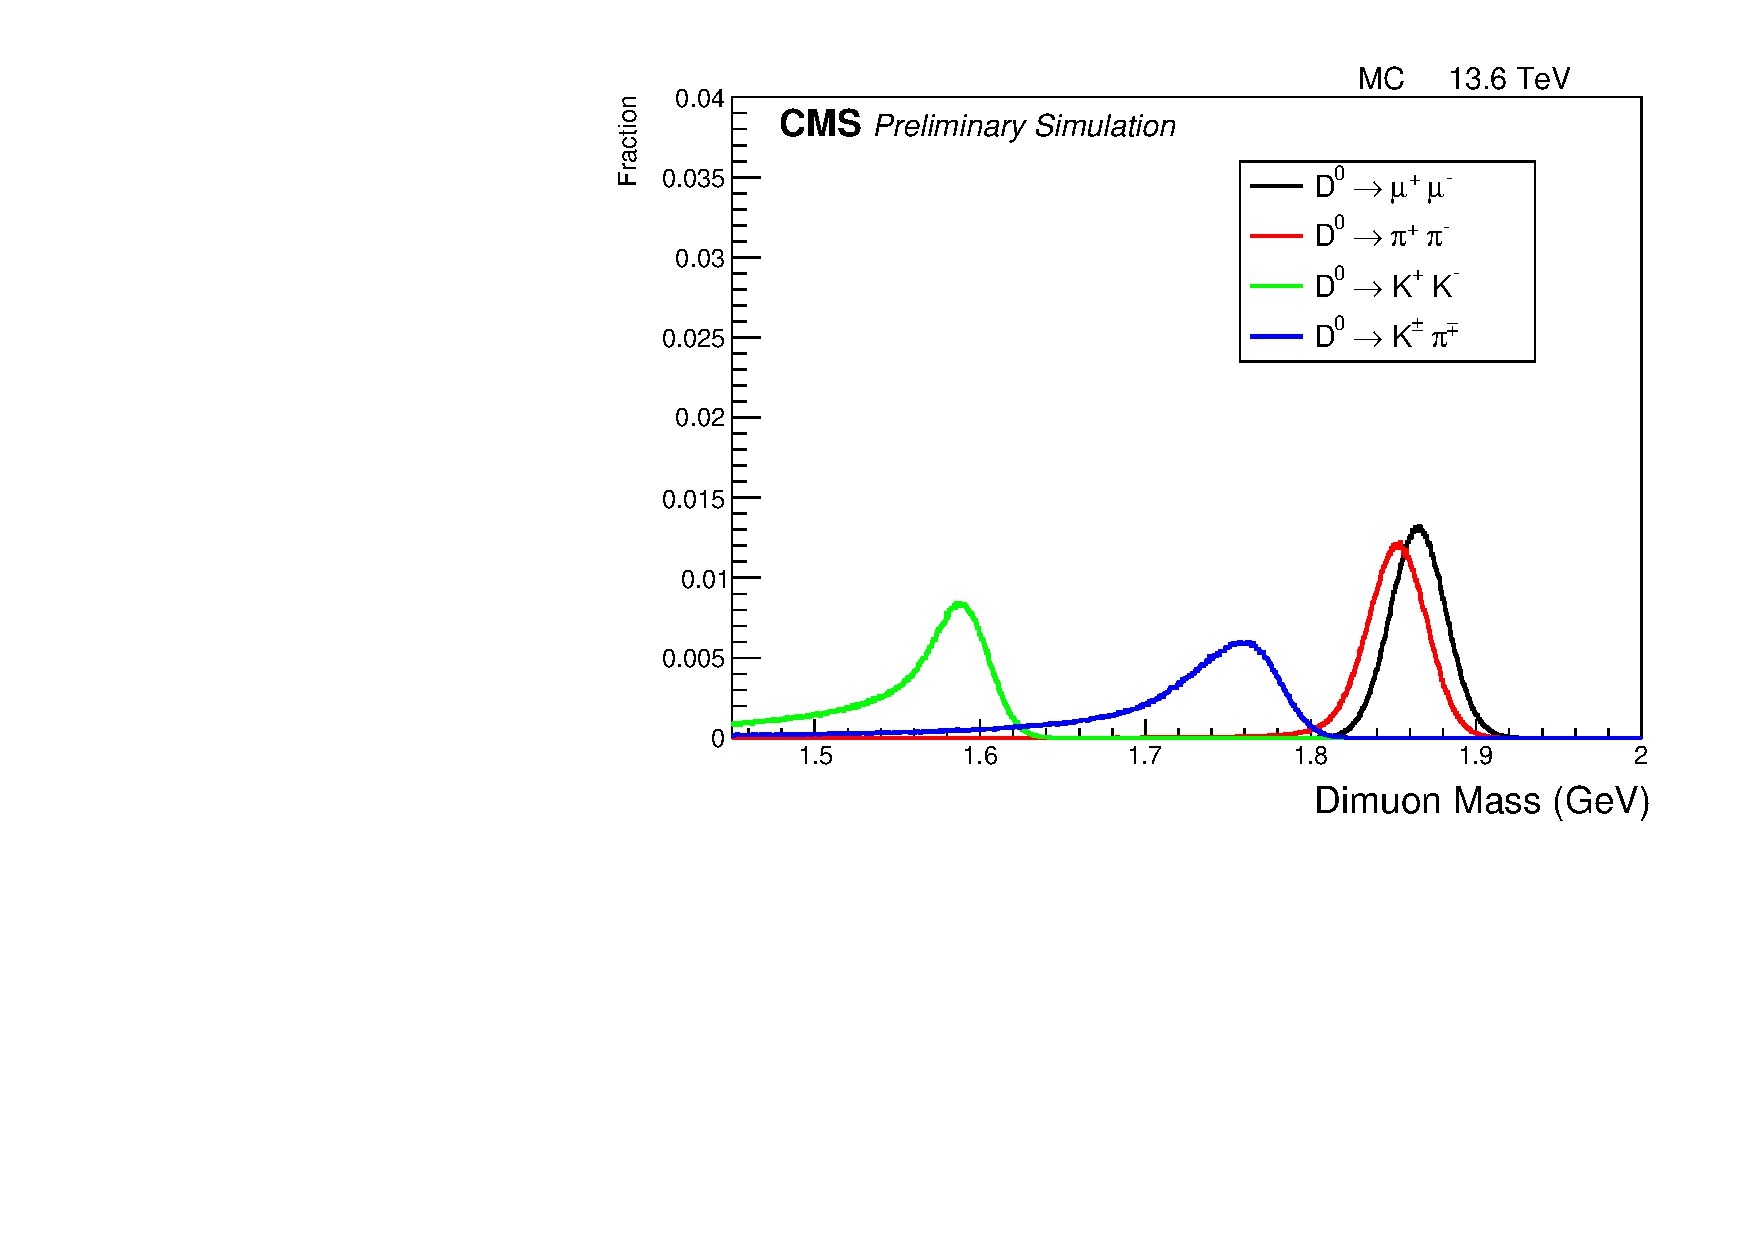
\includegraphics[width=0.45\textwidth]{figures/chapter4/reconstructed_D0_mass.pdf}
      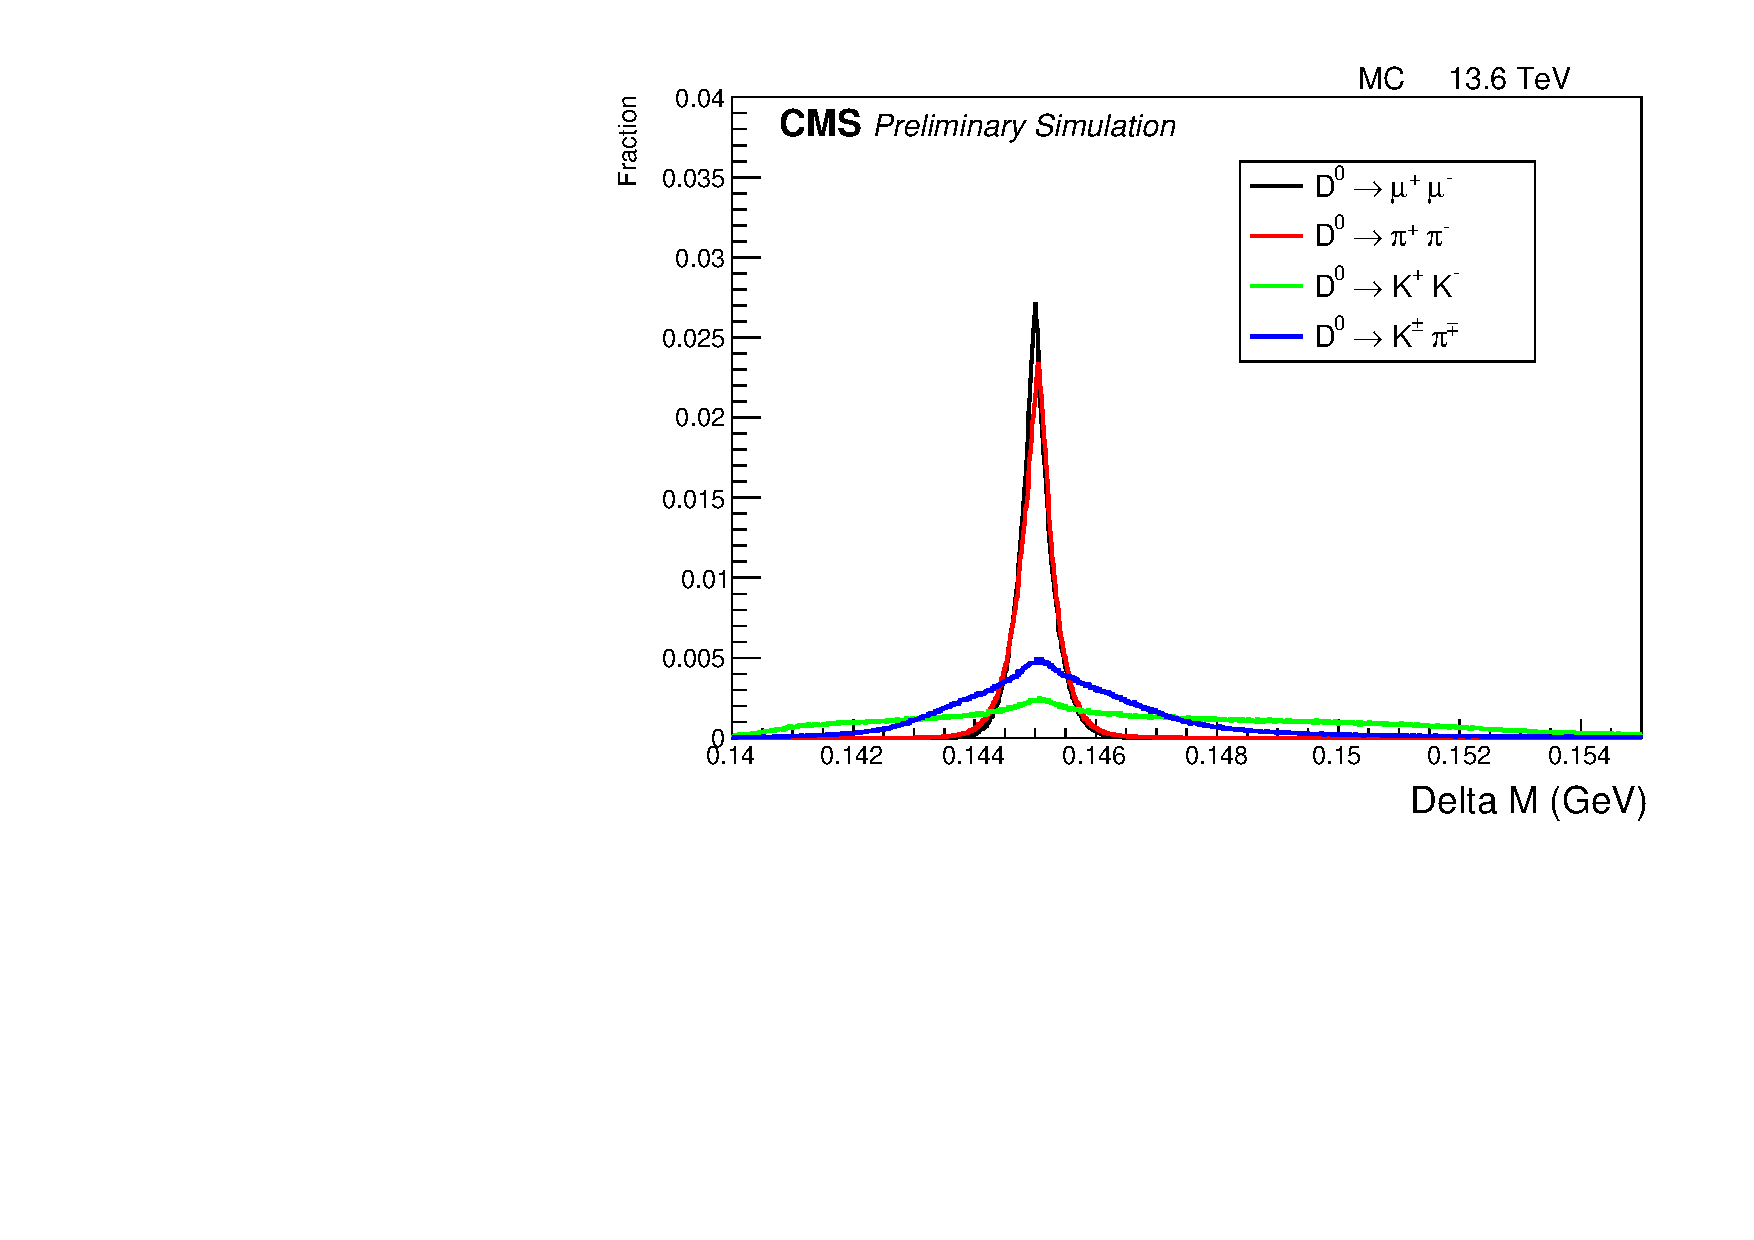
\includegraphics[width=0.45\textwidth]{figures/chapter4/reconstructed_delta_m.pdf}\\
    \end{center}
    \caption{
      Comparison of normalized frequencies for various peaking background $D^0 \to \mu^+ \mu^-$ decays against the signal decay.
      Right: Reconstructed $\Delta m$ distribution.
      Left: Reconstructed dimuon mass distribution, where decay products are forced to take the muon mass using \texttt{TGenPhaseSpace}, even for non-dimuon final states.
    }
    \label{fig:reconstructed_D0_comparison}
  \end{figure}
  
  


\subsection{Monte Carlo samples}

The main component of constructing the Monte Carlo (MC) simulation samples is properly modeling the $D^*$ meson by replicating their production in the CMS detector. The $D^*$ has two primary production mechanisms at the LHC
\begin{enumerate}
    \item Production through hadronization of charm quark directly from the proton-proton collision, creating prompt $D^*$ mesons close to the primary vertex. 
    \item Production through decay of other $B$ hadrons, creating displaced $D^*$ mesons from a secondary vertex
\end{enumerate}

It is important to model both of these production mechanisms of the $D^*$ decay to generate a reliable MC simulation sample, therefore both are included in the MC sample. Specifically, the first method produces a prompt soft pion in the $D^*\pm \to D^0 \pi^\pm$ process while the second method produces a displaced soft pion, resulting in significant differences in vertex parameters used in reconstruction and classification. The full complexity of the MC samples extends beyond the scope of this thesis, but table \ref{tab:mc-samples} displays some of the most used samples.

\begin{table}
\centering
\begin{tabular}{|p{3.2cm}|p{12cm}|}
    \hline
    \textbf{Sample Name} & \textbf{Attributes} \\
    \hline
    DstarToD0Pi\_ & -- SoftQCD:nonDiffractive (MinBias) \\
    D0To2Mu\_ & -- force $D^* \to D^0\pi$, $D^0 \to \mu^+\mu^-$ decay \\
    MuFilter & -- $|\eta(D^*)| < 3.0$ \\
    & -- $|\eta(D^0)| < 3.0$ for $D^0$ from $D^*$ \\
    & -- $|\eta| < 2.6$, $p_T > 3.0$ for muons from $D^0$ \\
    \hline
    DstarToD0Pi\_ & -- SoftQCD:nonDiffractive (MinBias) \\
    D0To2Pi\_ & -- force $D^* \to D^0\pi$, $D^0 \to \pi^+\pi^-$ decay \\
    PiFilter & -- $|\eta(D^*)| < 3.0$ \\
    & -- $|\eta(D^0)| < 3.0$ for $D^0$ from $D^*$ \\
    & -- $|\eta| < 2.6$, $p_T > 3.0$ for pions from $D^0$ \\
    \hline
    DstarToD0Pi\_ & -- SoftQCD:nonDiffractive (MinBias) \\
    D0ToKPi\_ & -- force $D^* \to D^0\pi$, $D^0 \to K^-\pi^+$ decay \\
    KPiFilter & -- $|\eta(D^*)| < 3.0$ \\
    & -- $|\eta(D^0)| < 3.0$ for $D^0$ from $D^*$ \\
    & -- $|\eta| < 2.6$, $p_T > 3.0$ for pions from $D^0$ \\
    \hline
    DstarToD0Pi\_ & -- SoftQCD:nonDiffractive (MinBias) \\
    D0To2Pi\_ & -- force $D^* \to D^0\pi$, $D^0 \to \pi^+\pi^- \to \mu^+\nu_\mu\mu^-\nu_\mu$ \\
    PiToMuPiFilter\_ & -- reduce pion $c\tau$ from 7.8\,m to 15.6\,cm \\
    PiLifetime0p02 & -- pion decay limits: $R < 2$\,m, $|z| < 4$\,m \\
    & -- $|\eta(D^*)| < 3.0$ \\
    & -- $|\eta(D^0)| < 3.0$ for $D^0$ from $D^*$ \\
    & -- $|\eta| < 2.6$, $p_T > 3.0$ for pions from $D^0$ \\
    & -- $|\eta| < 2.6$, $p_T(\mu) > 3.0$ for muons from pions \\
    \hline
\end{tabular}
\caption{The 4 most relevant MC simulation samples and their defining attributes.}
\label{tab:mc-samples}
\end{table}

\section{Selections and efficiency}
\label{sec:selections_and_efficency}

Once we've attained the data and MC samples needed for this analysis, we filter through them using event selections, carefully tracking the \textit{acceptance} and \textit{efficiency} for each selection\footnote{We define \textit{acceptance} as the purely kinematic fraction of signal events that fall inside the geometric phase space of the analysis and \textit{efficiency} as the analysis' performance in identifying signal events that are inside the geometric region}. The selection process can be broken down into three main stages:
\begin{enumerate}
    \item The \textit{preselection} stage provides the selections which are tied to trigger requirements, reconstruction requirements, and dataset size limitations.
    \item The \textit{baseline selection} stage primarily is used to reject background samples while keeping the efficiency high, the sidebands of the signal region large, and the signal shape unperturned. 
    \item The \textit{multivariate analysis (MVA) selection} stage uses ML-methods to optimize the background rejection.
\end{enumerate}

\subsection{Preselection}
\label{subsec:preselection}

The preselection is used to create reconstructed event candidates which pass the triggers discussed in section \ref{subsec:data_samples}. To stay consistent between signal and normalization events, we keep a similar preselection process for both $D^{*\pm} \to D^0 \pi^\pm, D^0 \to \mu^+ \mu^-$ and $D^{*\pm} \to D^0 \pi^\pm, D^0 \to \pi^+ \pi^-$ events.

In order to properly reconstruct the $D^{*\pm} \to D^0 \pi^\pm, D^0 \to \mu^+ \mu^-$ and $D^{*\pm} \to D^0 \pi^\pm, D^0 \to \pi^+ \pi^-$ events, we first must reconstruct their decay products: the muons and pion. Pions are reconstructed from charged tracks found in the tracker. These track are reconstructed using particle flow (PF) algorithms\footnote{The primary goal of these algorithms is to reconstruct individual particles using the data read out from the detector itself. This is made especially difficult because of the high lumonisties of run3 resulting in a large amount of \textit{pileup}, a phenomenon that occurs due to multiple proton-proton collisions happening within a very short time frame resulting in multiple collisons per event. }, meaning the pions used in the analysis are labeled as PF candidates. Muons are reconstructed primarily using detector read out from the muon chambers. We use the well established CMS reconstruction algorithms \texttt{TrackerMuon} and \texttt{GlobaleMuon} as well as use the collaboration's \texttt{LooseMuonID} for muon identification. To reduce background noise and increase detector resolution, we also cut at $p_T>4$ GeV and require a \texttt{highPurity} inner track in the tracker for both pions and muons.

Once we have the muon and/or pion candidates for the $D^0$ decay, we use vertex reconstruction to reconstruct the full decay candidate. A \textit{vertex} is the location in 3D space where a process occured and the \textit{primary vertex} is the location of the interaction of the quarks of the two colliding protons, which in our case produce the $D^{*\pm}$. Due to the short mean lifetime of the $D^{*\pm}$ ($ 6.9 \pm 1.9 \times 10^{-21} \; s$) \cite{ref:pdg2024}, we can label the $D^{*\pm} \to D^0 \pi^\pm$ vertex using the primary vertex. The kinematic vertex reconstruction begins by identifying the dimuon or dipion decay candidates fit to a common vertex (i.e two pions or two muons which came from the same decay). The two 4-momentum vectors of these two candidates is added together to get a dimuon or dipion 4-momentum vector. We call this dimuon/dipion system a $D^0$ candidate. Using the $D^0$ candidate 4-momentum vector, we calculate the transverse momentum of $D^0$ candidate and extrapolate it to its intersection with the beamline. Then, in order to determine which primary vertex\footnote{There are often many primary vertices in one event due to pileup} the $D^{*\pm} \to D^0 \pi^\pm$ decay came from, we calculate the 3D distance between each primary vertex candidate and the extrapolated intersection point, known as the \textit{3D-impact parameter}, and find the primary vertex which minimizes this parameter. Lastly, since the decay at the primary vertex is $D^{*\pm} \to D^0 \pi^\pm$, we check if there exists a soft pion which came from the selected primary vertex. This kinematic vertex reconstruction is then used to gather reconstructed signal and normalization events as well as refit the $D^0$ candidates to a common vertex using a kinematic vertex fitting tool, generating \textit{refitted} candidates. The events which pass this reconstruction are thus the events that pass the preselection. 

\begin{figure}[htbp]
    \centering
    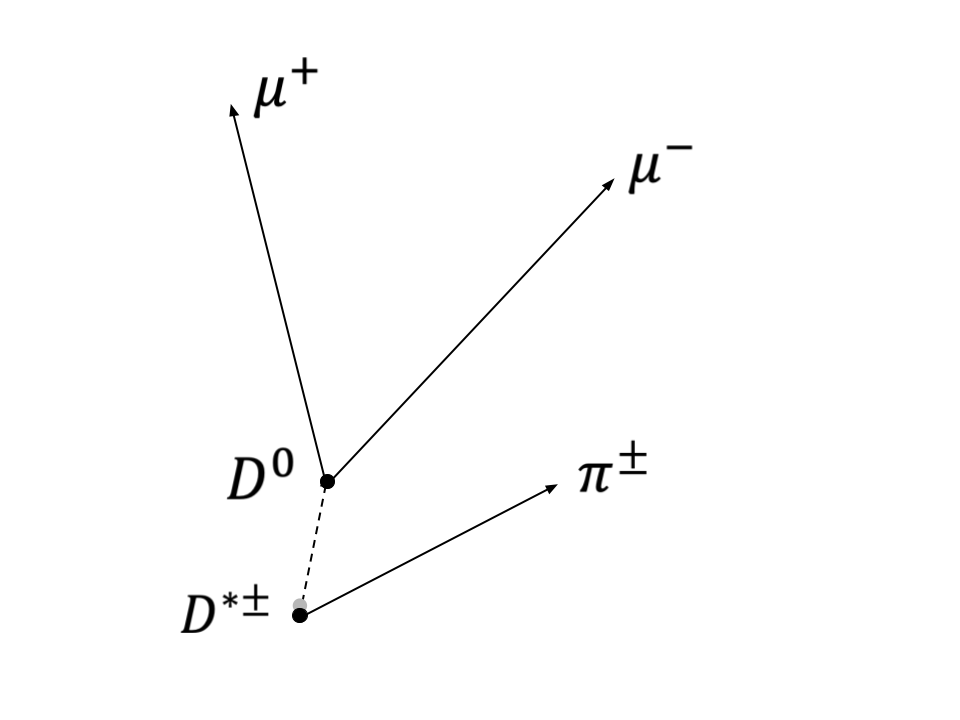
\includegraphics[width=0.8\textwidth]{figures/chapter4/vertex_reconstruction.png}
    \caption{An example of the $D^{*\pm} \to D^0 \pi^\pm, D^0 \to \mu^+ \mu^-$ vertex}
    \label{fig:vertex_reconstruction}
\end{figure}

\subsection{Baseline selection}
\label{subsec:baseline_selection}

Using the reconstruction described in section \ref{subsec:preselection}, we are able to extract several kinematic variables from $D^{*\pm} \to D^0 \pi^\pm$ candidates outputted by the preselection. These variables are used in the baseline selection as well as in other parts of the analysis. They are defined here as follows:
\begin{enumerate}
    \item Reconstructed $D^0$ mass: the mass calculated from from the addition of the two 4-momentum vectors of the $D^0$'s product candidates (either dimuon or dipion). 
    \item Refitted $D^0$ mass: the mass calculated from from the addition of the two 4-momentum vectors of the $D^0$'s product candidates (either dimuon or dipion) once they have been refitted using the kinematic vertex fitting. 
    \item Reconstructed $\Delta m$: the mass difference between the reconstructed $D^{*\pm}$ candidates and the reconstructed $D^0$ candidates. 
    \item Refitted $\Delta m$: the mass difference between the $D^{*\pm}$ and the $D^0$ candidates once they have been refitted using the kinematic vertex fitting.
    \item $\delta_{3D}$: the 3D impact parameter as defined in section \ref{subsec:preselection})
    \item $\delta_{3D}/\sigma\left(\delta_{3D}\right)$: the significance of the 3D impact parameter. This is calculated by taking the value of the 3D impact parameter and dividing it by the square root of the expected variance of the parameter. 
    \item $l_{3D}$: the 3D distance between the vertex of the $D^{*\pm} \to D^0 \pi^\pm$ decay (primary vertex) and the vertex of the $D^0 \to l l$ decay. This can also be called the $\textit{flight length}$ of the $D^0$ meson. 
    \item $l_{3D}/\sigma\left(l_{3D}\right)$: the significance of the 3D distance between the vertex of the $D^{*\pm} \to D^0 \pi^\pm$ decay (primary vertex) and the vertex of the $D^0 \to l l$ decay. Calculated by taking the value of the distance and dividing it by the square root of the expected variance of the distance. 
    \item $l_{xy}$: the distance in the $xy$ plane (perpendicular to the beam line) between the vertex of the $D^{*\pm} \to D^0 \pi^\pm$ decay (primary vertex) and the vertex of the $D^0 \to l l$ decay.  This can also be called the $\textit{transverse flight length}$ of the $D^0$ meson. 
    \item $l_{xy}/\sigma\left(l_{xy}\right)$: the significance of the distance in the $xy$ plane between the vertex of the $D^{*\pm} \to D^0 \pi^\pm$ decay (primary vertex) and the vertex of the $D^0 \to l l$ decay. Calculated by taking the value of the distance and dividing it by the square root of the expected variance of the distance. 
    \item $\alpha_{3D}$ : the angle between the $D^0$ momentum and flight direction. 
    \item $D^0$ vertex probability: the probability given by the $\chi^2$ fit which reconstructs the $D^0$ vertex 
    \item $D^*$ vertex probability: the probability given by the $\chi^2$ fit which reconstructs the $D^*$ vertex
\end{enumerate}
Note that, unless otherwise stated, the refitted variables are used over the reconstructed ones. 

Using these variables, we impart a baseline selection on the preselected events. The goal of the baseline selection is to reject much of the background while keeping the signal efficiency high and not perturbing the signal shape. To achieve this, we select a $D^0$ reconstructed mass in the range of [1.75, 1.95], $D^0$ refitted mass in the range of [1.81, 1.94], reconstructed $\Delta m$ in the range of [0.135, 0.160], and refitted $\Delta m$ in the range [0.140, 0.150]. These ranges are picked such that there are large sidebands on the signal, keeping signal efficiency high.

The other set of baseline selections are on the vertices themselves. We require the $D^*$ vertex probability to be greater that $0.1$ and the $D^0$ vertex probability to be greater than $0.01$. This is done such that there is some confidence in the vertex reconstruction and such that we can match the double muon trigger requirement of $0.005$. To gain further confidence in the vertex reconstruction, we limit $\alpha_{3D} < 0.1$ radians and the flight length significance to be greater than 3. Lastly, to keep the normalization channel (which is gathered from a ZeroBias trigger) under the same selection as the signal channel (which is gather from a HLT\_DoubleMuon trigger), we require the event in the normalization channel to have fired the \texttt{HLT\_DoubleMu4\_3\_LowMass} trigger. Note, this does not mean than the specific decay we reconstruct fired the trigger, in fact usually some other event has fired the trigger. 

%TODO: insert table of efficiencies


\subsection{Multivariate Analysis}
\label{subsec:mva}

The preselection and baseline selections optimize signal efficiency, but not overall analysis sensitivity. In order to optimize the analysis sensitivity, we train a classifier using a decision tree model driven multivariate analysis (MVA). This single classifying parameter can then be used as a selection parameter named $\text{MVA}_D$ and the cut can be tuned to optimize analysis sensitivity.

The decision tree model used is based on the XGBoost (Extreme Gradient Boosting) library, which builds a forest of regression trees trained sequentially to minimize a regularized objective function. Each tree in the sequence focuses on correcting the erros of the previous tree and the scores from the trees are combined to get a final prediction on the classifiction of the event from the forest. Each tree is constructed using a greedy algorithm that selects splits based on gain, with regularization terms penalizing model complexity to prevent overfitting. The loss function is binary logistic loss, which is optimized using boosting under second-order gradient information with an evaluation metric based on the area under the receiver-operating characteristic (ROC) curve, known as AUC in the literature. Each tree has a maximum depth of 3 and is trained using a learning rate of $\eta = 0.1$. An additional regularization is applied with an L1 penalty. A minimum loss reduction threshold for tree splits\footnote{This requirement only allows additional trees to form if their contribution causes the loss to decrease by some number, set in this analysis to be $2.0$} and a sub-sample ratio\footnote{This is the fraction of training data that each tree sees, which for this analysis is kept (as is standard) at $60\%$} are employed to additionally prevent overfitting. The model is trained for over 4000 epochs in each training round.

The signal events used for training are taken from simulated $D^0 \to \mu^+ \mu^-$ MC samples. The background events are taken from the data sidebands using the $\Delta m$ parameter with a distance of over $5\sigma$ right of the expected value ($\Delta m \in [0.150, 0.155]$ GeV) and dimuon mass in the signal range of $[1.81, 2.45]$ GeV. The dimuon mass is kept in the signal range to align the training data with not obviously rejected events. Should the background training data be selected outside the signal dimuon mass window, the classification of signal and background events would become trivial, leading to a less effective model.

The variables used in the training are
\begin{enumerate}
    \item The $p_T$ of both muons and the soft pion
    \item The $D^0$ vertex parameters, including point angle, flight length significance, vertex probability, 3D impact parameter, and significance of the 3D impact parameter.
    \item The $D^*$ vertex probability.
    \item The $D^0$ mass resolution over the $D^0$ mass.
\end{enumerate}

\begin{figure}[htp]
    \begin{center}
      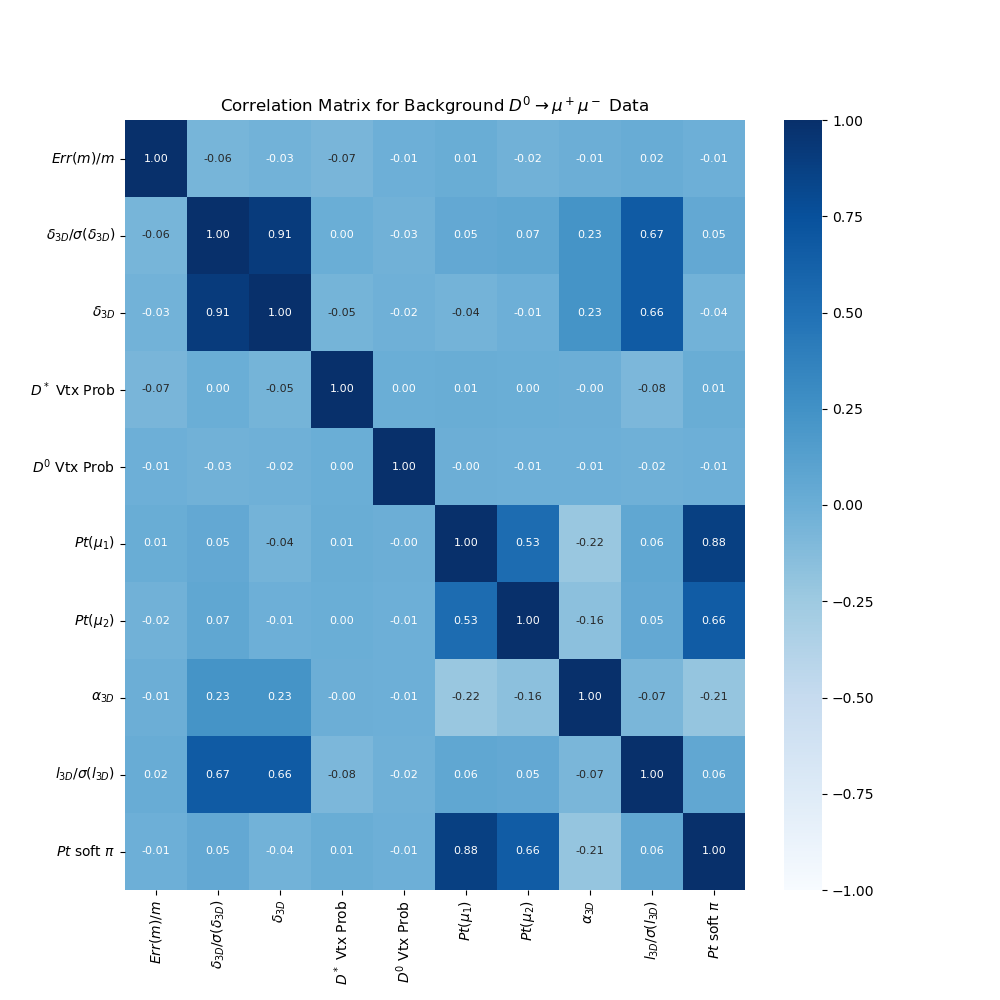
\includegraphics[width=0.45\textwidth]{figures/chapter4/mva/Correlation_data.png}
      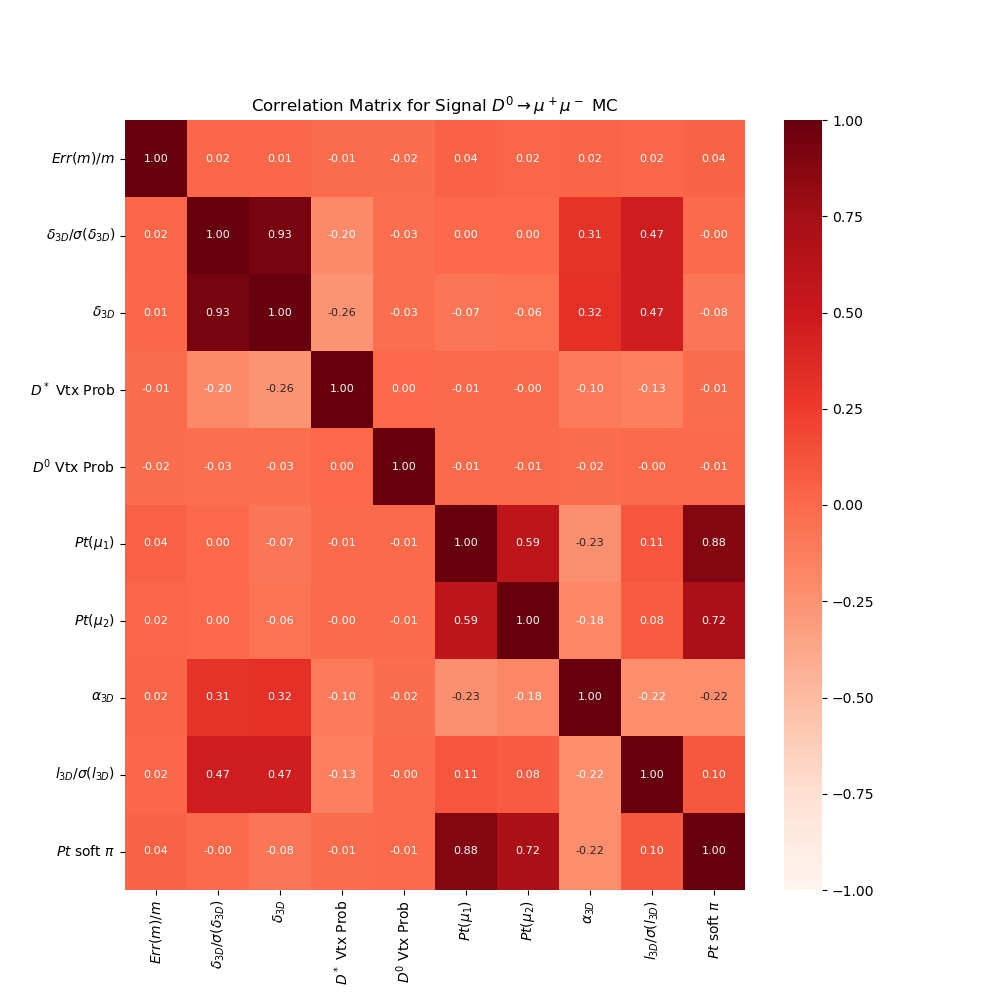
\includegraphics[width=0.45\textwidth]{figures/chapter4/mva/Correlation_dmm.png}\\
    \end{center}
    \caption{
      Correlation matrix over the MVA training variables for training background events generated from data (left) and training signal events generated from MC (right)
    }
    \label{fig:mva_correlation_matrix_for_training_variables}
\end{figure}

The correlation matrix for both the signal and background can be seen in figure \ref{fig:mva_correlation_matrix_for_training_variables}. Importantly, there are some positive correlation between features and there are no two strong anti-correlated features, meaning we expect stability in learning due to feature redundancy and simpler interactions, yet expect good model generalization. 

Due to the relatively small amount of data available, the data is split into 5 groups and 5 separate models are training, each using a different data group as testing data sets and the remaining 4 as training datasets. This ensures the models have been exposed on the entire dataset while not overfitting on any particular events. Once the models have been trained, the event number (which is independent of the contents of the event), is used to decide which model to use for classification of that event. 

It is important that the classification parameter is not correlated with any variables used later in the analysis for fitting (namely $\Delta m$ and the dimuon mass) so as to not skew the fit. Due to this, the kinematic variable given to the model are restricted to $p_T$ and vertex parameters, so that it is not possible to reconstruct masses. To check that the correlations don't exist, a correlation matrix between the classification parameter, $\Delta m$, and the dimuon mass is created and shown in figure \ref{fig:mva_correlation_matrix_for_fit_variables}. As expected, there is no correlation.


\begin{figure}[htp]
    \begin{center}
      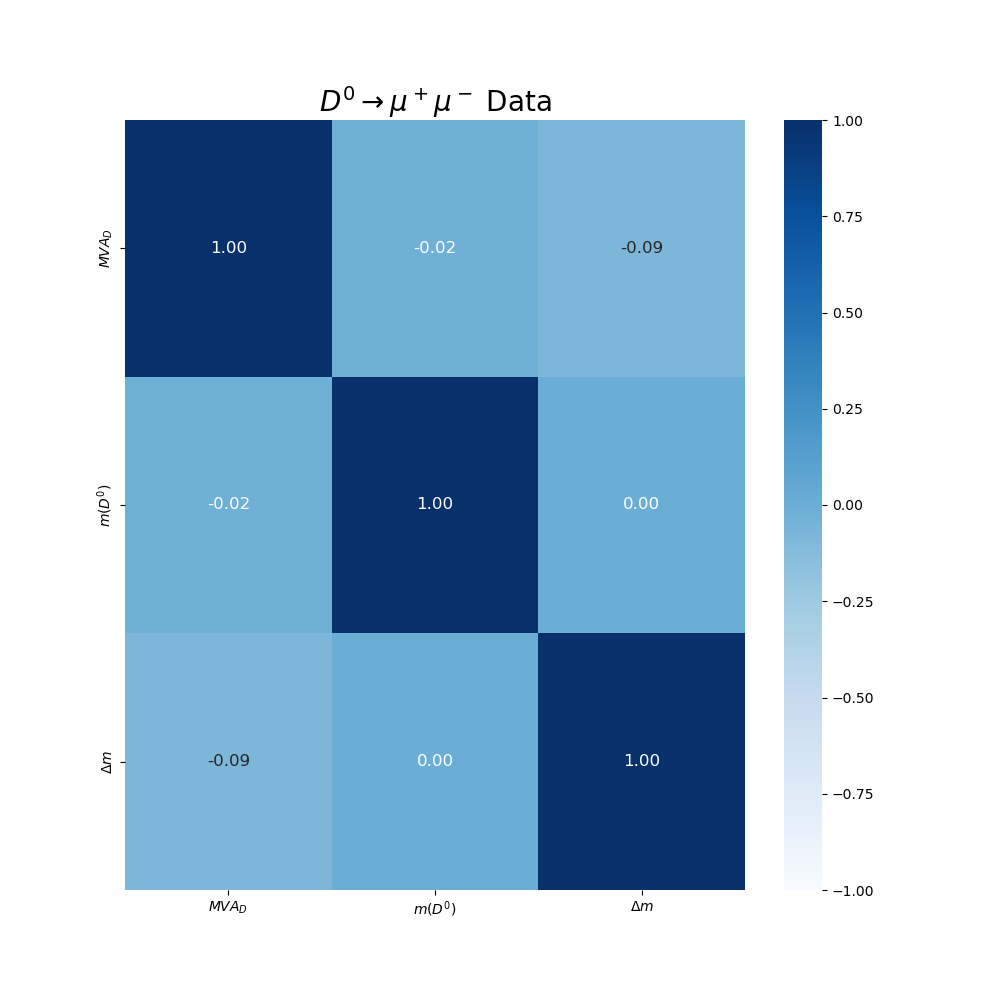
\includegraphics[width=0.45\textwidth]{figures/chapter4/mva/Correlation_data_obs.png}
      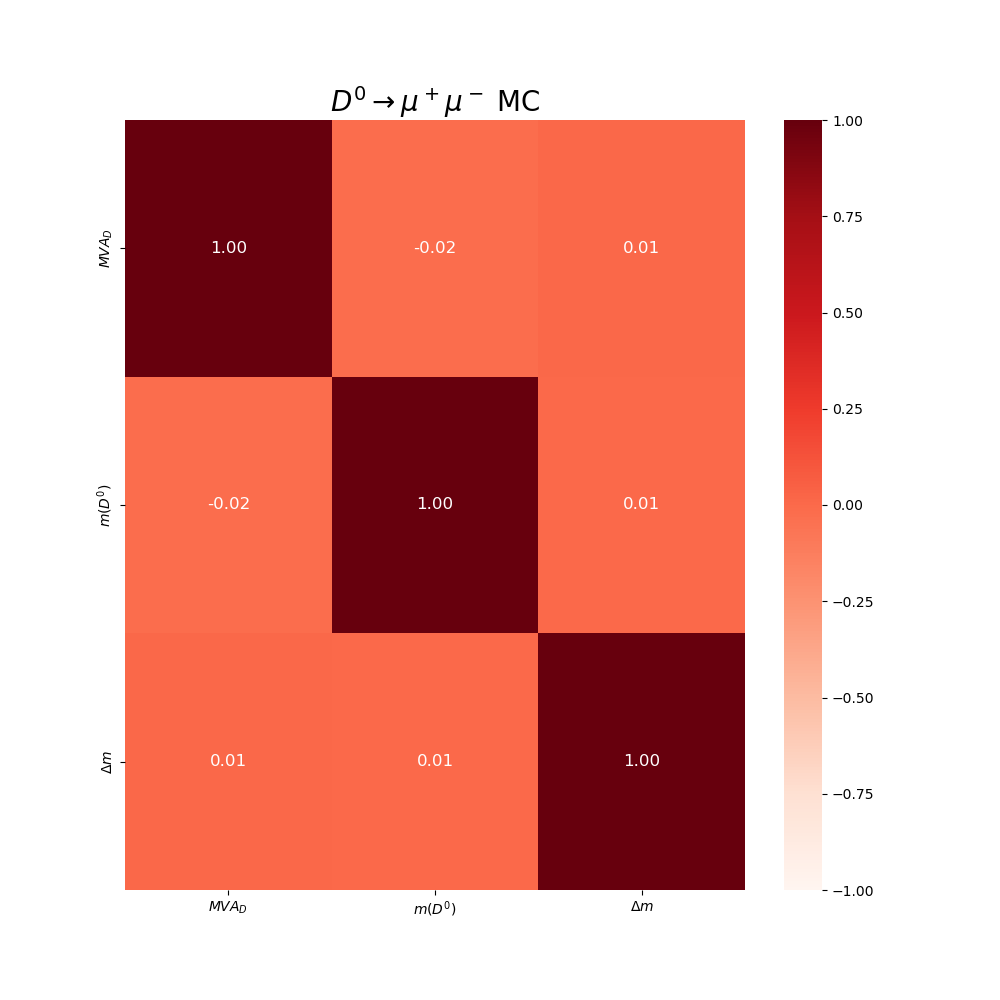
\includegraphics[width=0.45\textwidth]{figures/chapter4/mva/Correlation_dmm_obs.png}\\
    \end{center}
    \caption{
      Correlation matrix comparing the MVA classification parameter to $\Delta m$ and the dimuon mass. Shown left is the training background events generated from data and shown right is the training signal events generated from MC.
    }
    \label{fig:mva_correlation_matrix_for_fit_variables}
\end{figure}

% TODO: add statement about how efficiency is calculated in this analysis using simulated data
It is also important to note that the classifier is being trained and tested on simulated signal samples, yet for the analysis the efficiency of the classifier on real data is needed. Due to mismodeling effect in the simulation, the simulation efficiency is not necessarily the same as the data efficiency. Getting the efficiency is difficult to measure directly since the expected branching fraction of $D^0 \to \mu^+ \mu^-$ is so low that we do not have a reliable data sample for the signal. Instead, the efficiency is derived from the $D^0 \to \pi^+ \pi^-$ decay using the zero bias dataset and the $D^0 \to \pi^+ \pi^-$ monte-carlo simulation samples. Since the $D^0 \to \pi^+ \pi^-$ decay behaves similarly to the $D^0 \to \mu^+ \mu^-$ decay in terms of reconstruction/vertex parameters and the MVA classifier is independent of $\Delta m$ and dimuon mass in both cases, the efficiency derived from $D^0 \to \pi^+ \pi^-$ is similar to the efficiency of $D^0 \to \mu^+ \mu^-$. Therefore, the same classifier with the same cut is used on both the normalization channel and the signal channel, causing the efficiencies to cancel in the branching fraction equation (equation \ref{eq:main_analysis}). We calculate the efficiency in data on the $D^0 \to \pi^+ \pi^-$ decay by performing the UML fit outlined in section \ref{subsec:normalization_channel_fit} on different $\text{MVA}_D$ cut values and comparing to the \texttt{ZeroBias} dataset. In simulated data, we are able to directly tag the signal events that were created from the simulation, so calculating the efficiency is trivial. A list of efficiency values at specific $\text{MVA}_D$ cuts can be found in table \ref{tab:mva_cut_efficiencies} and a graphical representation over a more diverse $\text{MVA}_D$ cut range can be found in \ref{fig:mva_cut_efficiencies}.

\begin{table}[htbp]
    \centering
    \begin{tabular}{|l|c|c|c|}
    \hline
    $\text{MVA}_D$ cut value & \textbf{0.74} & \textbf{0.76} & \textbf{0.78} \\
    \hline
    $D^0 \to \pi^+ \pi^-$ Data Efficiency (from Zero Bias) & $0.722 \pm 0.088$ & $0.707 \pm 0.087$ & $0.681 \pm 0.086$ \\
    $D^0 \to \pi^+ \pi^-$ MC Efficiency & 0.817 & 0.801 & 0.783 \\
    $D^0 \to \mu^+ \mu^-$ MC Efficiency & 0.824 & 0.809 & 0.792 \\
    $D^0 \to \pi^+ \pi^- \to \mu^+\nu_\mu\mu^-\bar{\nu}_\mu$ MC Efficiency & 0.806 & - & - \\
    \hline
    \end{tabular}
    \caption{Summary of $\text{MVA}_D$ cut efficiency at various cut values on various samples used throughout the analysis.}
    \label{tab:mva_cut_efficiencies}
\end{table}

\begin{figure}[htp]
    \begin{center}
      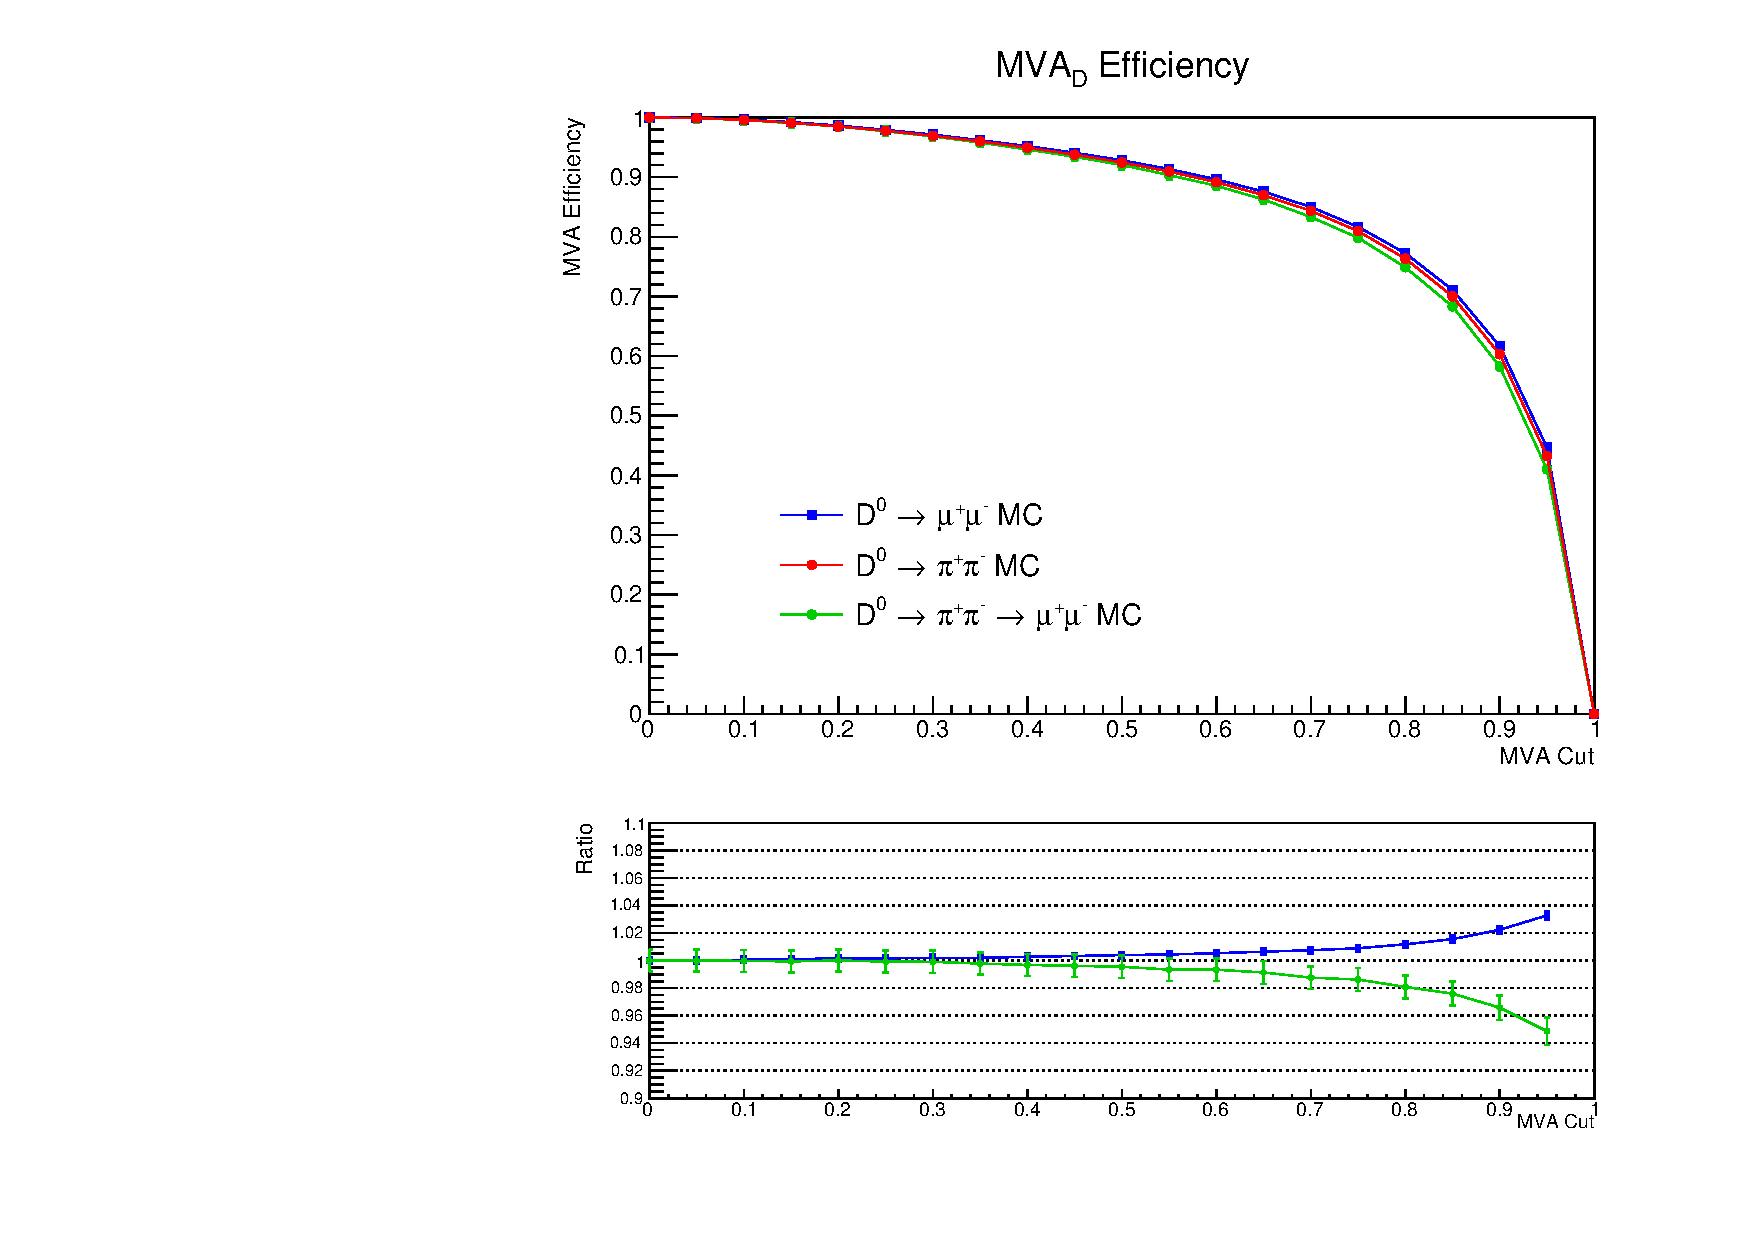
\includegraphics[width=0.5\textwidth]{figures/chapter4/mva/mva_efficiency.pdf}
    \end{center}
    \caption{
      A graphical summary of $\text{MVA}_D$ cut efficiency at various diverse cut values on various samples used throughout the analysis.
    }
    \label{fig:mva_cut_efficiencies}
\end{figure}

As can be seen in table \ref{tab:mva_cut_efficiencies} as well as figure \ref{fig:mva_cut_efficiencies}, while the efficiency values are, as expected, extremely close in the MC samples, there is still a small difference between the three decay channels. To account for this small difference, we calculate a corrective efficiency factor, derived from MC. We name this corrective factor $\text{MVA}_{D, cor}$ and define it as
\begin{equation}
    \begin{split}
    \text{MVA}_{D,\text{cor}\;(D^0 \to \mu^+ \mu^-)} &= 
    \frac{\epsilon_{D^0 \to \mu^+ \mu^-\; \text{ (simulation)}}}
         {\epsilon_{D^0 \to \pi^+ \pi^-\; \text{ (simulation)}}} \\
    \text{MVA}_{D,\text{cor}\;(D^0 \to \pi^+ \pi^- \to \mu^+ \nu_\mu \mu^- \nu_\mu)} &= 
    \frac{\epsilon_{D^0 \to \pi^+ \pi^- \to \mu^+ \nu_\mu \mu^- \nu_\mu\; \text{ (simulation)}}}
         {\epsilon_{D^0 \to \pi^+ \pi^-\; \text{ (simulation)}}}
    \end{split}
\end{equation}
From these definitions, one can extrapolate to data due to the proximity of the efficiency values, meaning
\begin{equation}
    \begin{split}
    \epsilon_{D^0 \to \mu^+ \mu^-} \text{ (data)} &= 
    \epsilon_{D^0 \to \pi^+ \pi^-} \text{ (data)} 
    \times \text{MVA}_{D,\text{cor}\;(D^0 \to \mu^+ \mu^-)} \\
    \epsilon_{D^0 \to \pi^+ \pi^- \to \mu^+ \nu_\mu \mu^- \nu_\mu} \text{ (data)} &= 
    \epsilon_{D^0 \to \pi^+ \pi^-} \text{ (data)} 
    \times \text{MVA}_{D,\text{cor}\;(D^0 \to \pi^+ \pi^- \to \mu^+ \nu_\mu \mu^- \nu_\mu)}
    \end{split}
\end{equation}
Lastly, a very conservative systematic error is assigned to the $\text{MVA}_{D, cor}$ factors of $|1-\text{MVA}_{D, cor}|$. Therefore, we get
\begin{equation}
\begin{split}
    \text{MVA}_{D,\text{cor}\;(D^0 \to \mu^+ \mu^-)} &= 1.009\;\pm\;0.012 \; \text{(stat)}\;\pm\;0.009 \; \text{(sys)} \\
    \text{MVA}_{D,\text{cor}\;(D^0 \to \pi^+ \pi^- \to \mu^+ \nu_\mu \mu^- \nu_\mu)} &= 0.987\;\pm\;0.020 \; \text{(stat)}\;\pm\;0.013 \; \text{(sys)}
\end{split}
\end{equation}
    
\section{Unbinned Maximum Likelihood Fits}
\label{sec:UML}

Now that we have given accurate descriptions of the datasets and selection processes used in this analysis, we are now ready to extract the two main values needed for this analysis, the number of $D^0 \to \pi^+ \pi^-$ events, denoted $N_{D^0 \to \pi^+ \pi^-}$, the number of $D^0 \to \mu^+ \mu^-$ events, denoted $N_{D^0 \to \mu^+ \mu^-}$.

In order to do this, we perform two unbinned maximum likelihood (UML) fits on the events in our data that passes the preselection, baseline selection, and MVA selection processes. Maximum likelihood (ML) fits are statistical methods used to estimated parameters of a model given observed data. A ML fit is a UML fit when the data is not binned into a histogram, but rather the exact data values are used. UML fits define a model $f(\vec{x}; \theta, \theta_N)$, which is a PDF over some set of observed variables, $\vec{x}$ and some model parameters $\theta$ and $\vec{\theta}_N$. The goal of a UML fit is to extract a model parameter $\theta$ given some observed data $\vec{x}_1, \vec{x}_2,...,\vec{x}_N$. $\vec{\theta}_N$ are considered nuisance parameters and are important to defining the model, but are not parameters of interest to the analysis. Once a model has been defined, a likelihood is defined as
\begin{equation}
    \mathcal{L}(\theta, \vec{\theta}_N) = \prod^N_{i=1} f(\vec{x}_i; \theta, \vec{\theta}_N)
\end{equation}
In this formulation, the UML fit can be represented as finding $\hat{\theta} \hat{\vec{\theta}_N}= \text{argmax}_{\theta, \vec{\theta}_N} \mathcal{L}(\theta, \vec{\theta}_N)$\footnote{In practice, this isn't quite true. Often in applications with lots of nuisance parameters, UML fits operate using profile likelihoods. However, the point of this discussion is merely an overview of UML and the complexities will be ignored.}. 

In our analysis, $\theta$ is the true number of signal events (in the normalization channel this is $N_{D^0 \to \pi^+ \pi^-}$ and in our signal channel this is $N_{D^0 \to \mu^+ \mu^-}$), $\vec{x}$ is the $\Delta m$ and $m(D^0)$ of our data, and $\vec{\theta}_N$ are the variance parameters needed to construct the signal and background PDFs. As can be seen in figure \ref{fig:mva_correlation_matrix_for_fit_variables}, there exists practically no correlation between $\Delta m$ and $m(D^0)$. This tells us that the 2D model can be split as a product of 1D models. More specifically, we have that
\begin{equation}
    f(\vec{x}; \theta, \theta_N) = f_{m(D^0)}(m(D^0); \theta, \theta_N) \times f_{\Delta m}(\Delta m; \theta, \theta_N)
\end{equation}

A more precise discussion of this construction follows in the sections below. For each of the two channels we begin by developing the models for both the signal and the background. Then, we outline the specifics of the fit and any corrections applied to it. Lastly, we outline the results of the fit. 

\subsection{Normalization Channel Fit}
\label{subsec:normalization_channel_fit}

The goal of the normalization channel is to extract $N_{D^0 \to \pi^+ \pi^-}$. This is done using the \texttt{HLT\_ZeroBias} trigger dataset, as is described in section \ref{subsec:data_samples}. Perhaps the largest difficulty of the UML fit on the normalization channel is that the \texttt{HLT\_ZeroBias} trigger dataset does not contain many of the $D^{*\pm}\to D^0 \pi^\pm, D^0 \to \pi^+ \pi^-$ signal events due the large prescaling factor of the trigger, discussed in section \ref{subsec:data_samples}. The below section, in part, describes in detail how this difficulty is overcome by using MC samples to inform the fit and correcting for MC mismodeling effects when needed in the final fit. 

\subsubsection{Signal Model}

The signal model for the normalization channel describes the $\Delta m$ and $m(D^0)$ of the $D^{*\pm}\to D^0 \pi^\pm, D^0 \to \pi^+ \pi^-$ decay. As is common to do for masses in signal distributions, the model for $m(D^0)$ is a sum of two Gaussian distributions forced to share a common mean. Similarly, the model for $\Delta m$ is a sum of three Gaussian distributions forced to share a common mean.

Due to the small number of signal events in data, the shape (composing of the means and standard deviations) of this model is determined by fits to simulated MC samples. This is because the shape will be much more stable in MC compared to data, simply just because there are more samples in MC. Once the shape is found using MC, it is frozen and only the number of events is allowed to float when the fit is applied to data. The signal model fit to MC can be seen in figure \ref{fig:d0pipi_uml_fit_pipi_model}.

\begin{figure}[htp]
    \begin{center}
      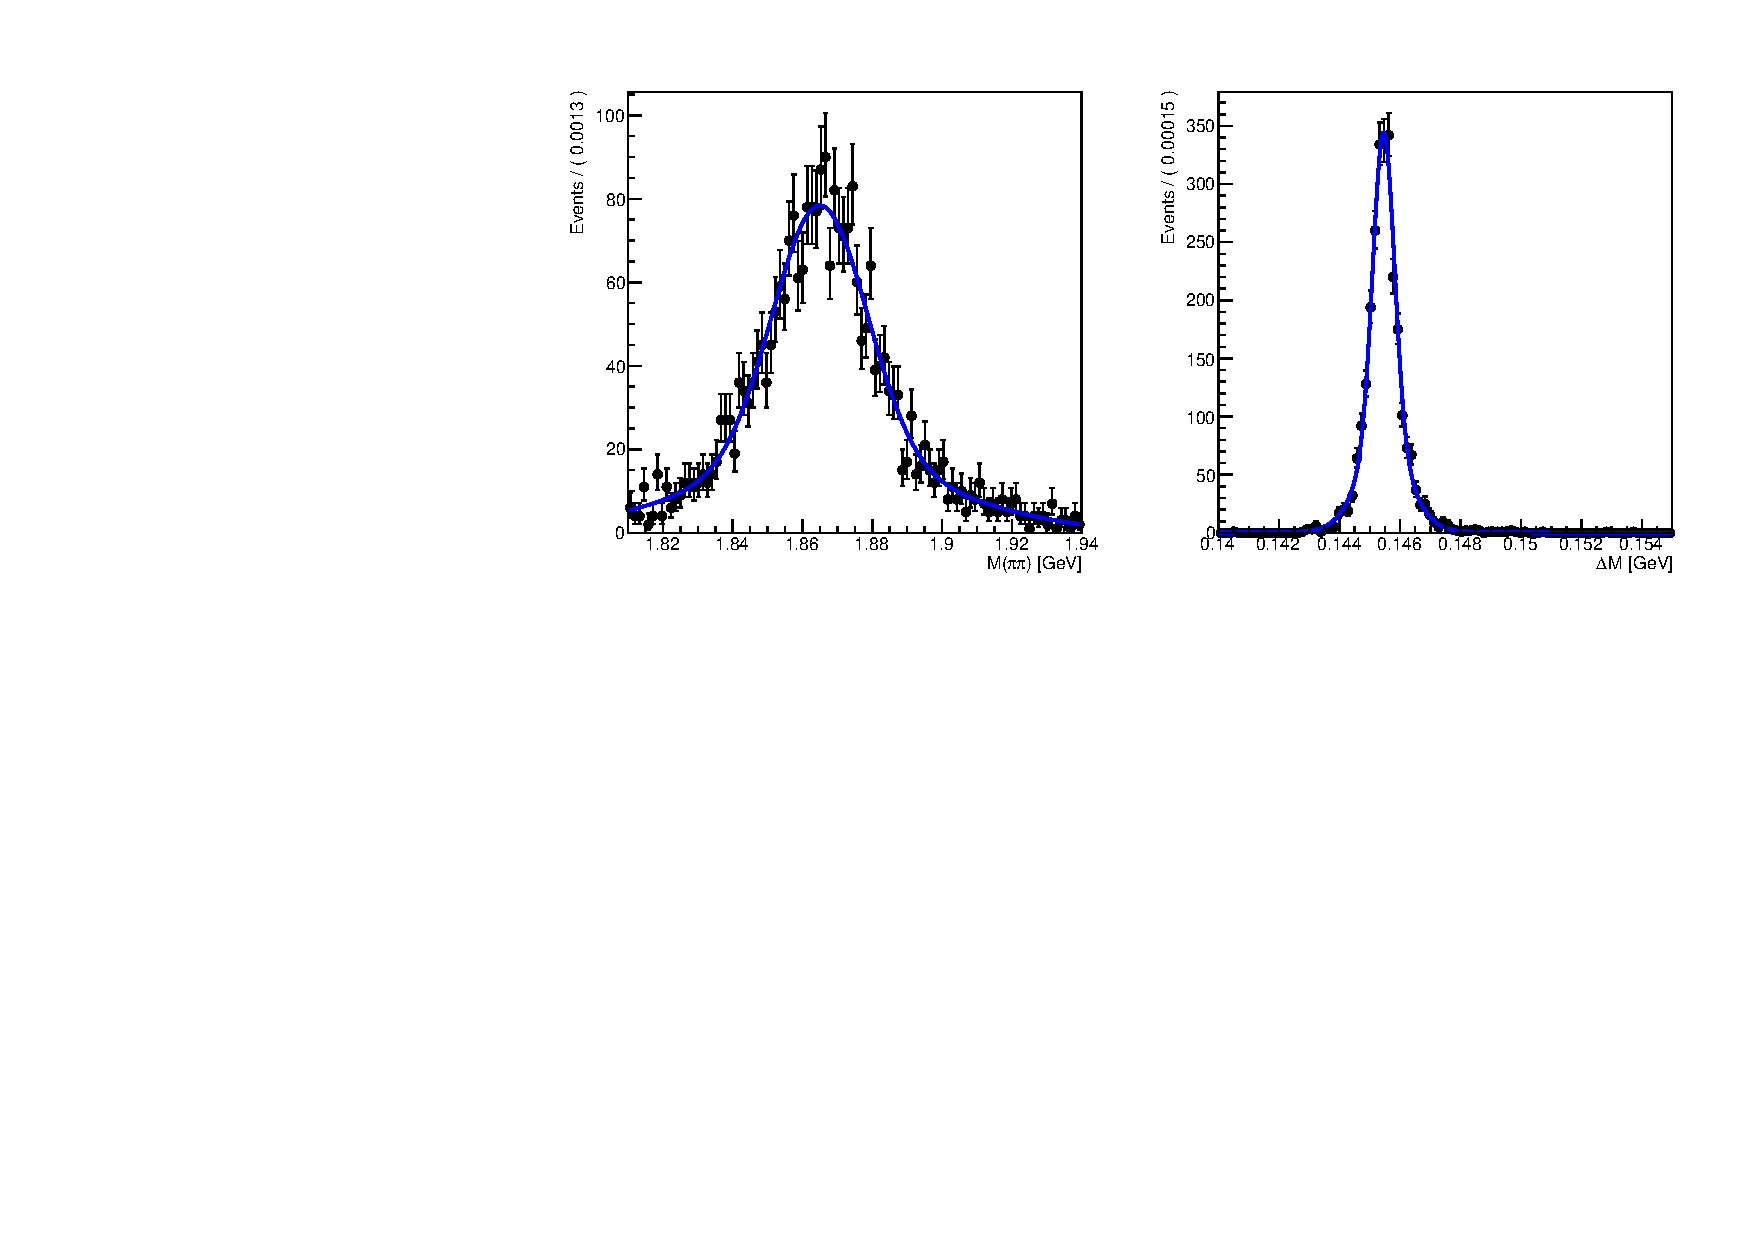
\includegraphics[width=0.9\textwidth]{figures/chapter4/normalization_fit/dpipi_fit_mc.pdf}
    \end{center}
    \caption{
      The signal model fit on MC samples, with $m(D^0)$ displayed left and $\Delta m$ displayed right.
    }
    \label{fig:d0pipi_uml_fit_pipi_model}
\end{figure}

It is possible, however, that the shape varies slightly between the MC samples and data, due to mismodeling in MC. To account for this slight mismodeling affect, we derive correction factors $\mu_{\text{corr}}$ and $\sigma_{\text{corr}}$ such that
\begin{equation}
\begin{split}
    \mu_{\text{data}} &= \mu_{\text{MC}} \times (1+\mu_{\text{corr}}) \\
    \sigma^i_{\text{data}} &= \sigma_{\text{MC}} \times (1+\sigma_{\text{corr}}) 
\end{split}
\label{eq:shape_correction_definition}
\end{equation}
where $i$ is used to denote that each of the models has multiple width parameters (one for each Gaussian distribution that is summed) but only one mean parameter.

To derive what this correction factor is, we use the \texttt{HLT\_DoubleMu4\_3\_LowMass} trigger to construct a dataset with enough signal samples to construct a reliable data-driven fit shape. We then run the full normalization channel UML fit (including the background models) on this data. Comparing that to the shape obtained from MC, we can easily derive the $\mu_{\text{corr}}$ from equation \ref{eq:shape_correction_definition}. 

Initially, it might seem that one could apply the same procedure to find $\sigma_{\text{corr}}$. However, this dimuon trigger enhances the amount of $b\bar{b}$ production in the sample, which biases the width of the $D^{*\pm}\to D^0 \pi^\pm, D^0 \to \pi^+ \pi^-$ decay. Therefore, one must first properly understand that bias before applying the correction in the same way as the mass was done. To understand the bias effect between the Dimuon and Zerobias triggers, we compare $D^{*\pm}\to D^0 \pi^\pm, D^0 \to K^\pm \pi^\mp$ fits from the Dimuon and Zerobias dataset. This is possible because the Kaon decay mode is much more frequent than the pion decay mode. The fitting process is the same as before and the width correction 
can be obtained as
\begin{equation}
    \begin{split}
        1+\sigma_{\text{corr}} &= \left(1+\sigma_{\text{corr, DoubleMuon}}^{D^0\to\pi^+\pi^-}\right) \\
        &\times \frac{
            1+\sigma_{\text{corr, ZeroBias}}^{D^0\to\pi^\pm\pi^\mp}
        }{
            1+\sigma_{\text{corr, DoubleMuon}}^{D^0\to K^\pm\pi^\mp}
        }
    \end{split}
\end{equation}    
%All of the corrections to the signal shape are summarized TODO: add table reference.

%TODO: add table of width corrections.  Likely won't do this

\subsubsection{Background Model}

As described in section \ref{subsec:backgrounds}, there are 3 peaking backgrounds and a combinatorial background to consider in the normalization channel. 

To begin, we describe the 3 peaking backgrounds. The first, as most prominant, of these three backgrounds is the $D^{*\pm} \to D^0\pi^\pm, D^0 \to K^\pm \pi^\mp$. As shown in figure \ref{fig:reconstructed_D0_comparison}, the $m(D^0)$ peak is shifted signficiantly to the left due to incorrect mass of the pion imposed on the kaon during reconstruction. In fact, the mean in shifted so far that only the tail of the Gaussian distribution persists in the mass region of our fit. Since the tail of a Gaussian distribution is approximately an exponential function, we use an exponential function to fit the $m(D^0)$ parameter. This fit proves to be significantly more stable as the exponential function only has one shape parameter that requires fitting while the Gaussian distribution has two. In contrast, the $\Delta m$ distribution of the $D^{*\pm} \to D^0\pi^\pm, D^0 \to K^\pm \pi^\mp$ decay closely follows the shape of the signal. Therefore, we similarly use a sum of three Gaussian distributions with a common mean do model the $\Delta m$ distribution. The convergence of the fit is verified using MC samples and is displayed in figure \ref{fig:d0pipi_uml_fit_kpi_model}. The data fit remains stable even when these shape parameters are allowed to vary. Therefore, we allow the shape of this peaking background to vary when fit to data. 

\begin{figure}[htp]
    \begin{center}
      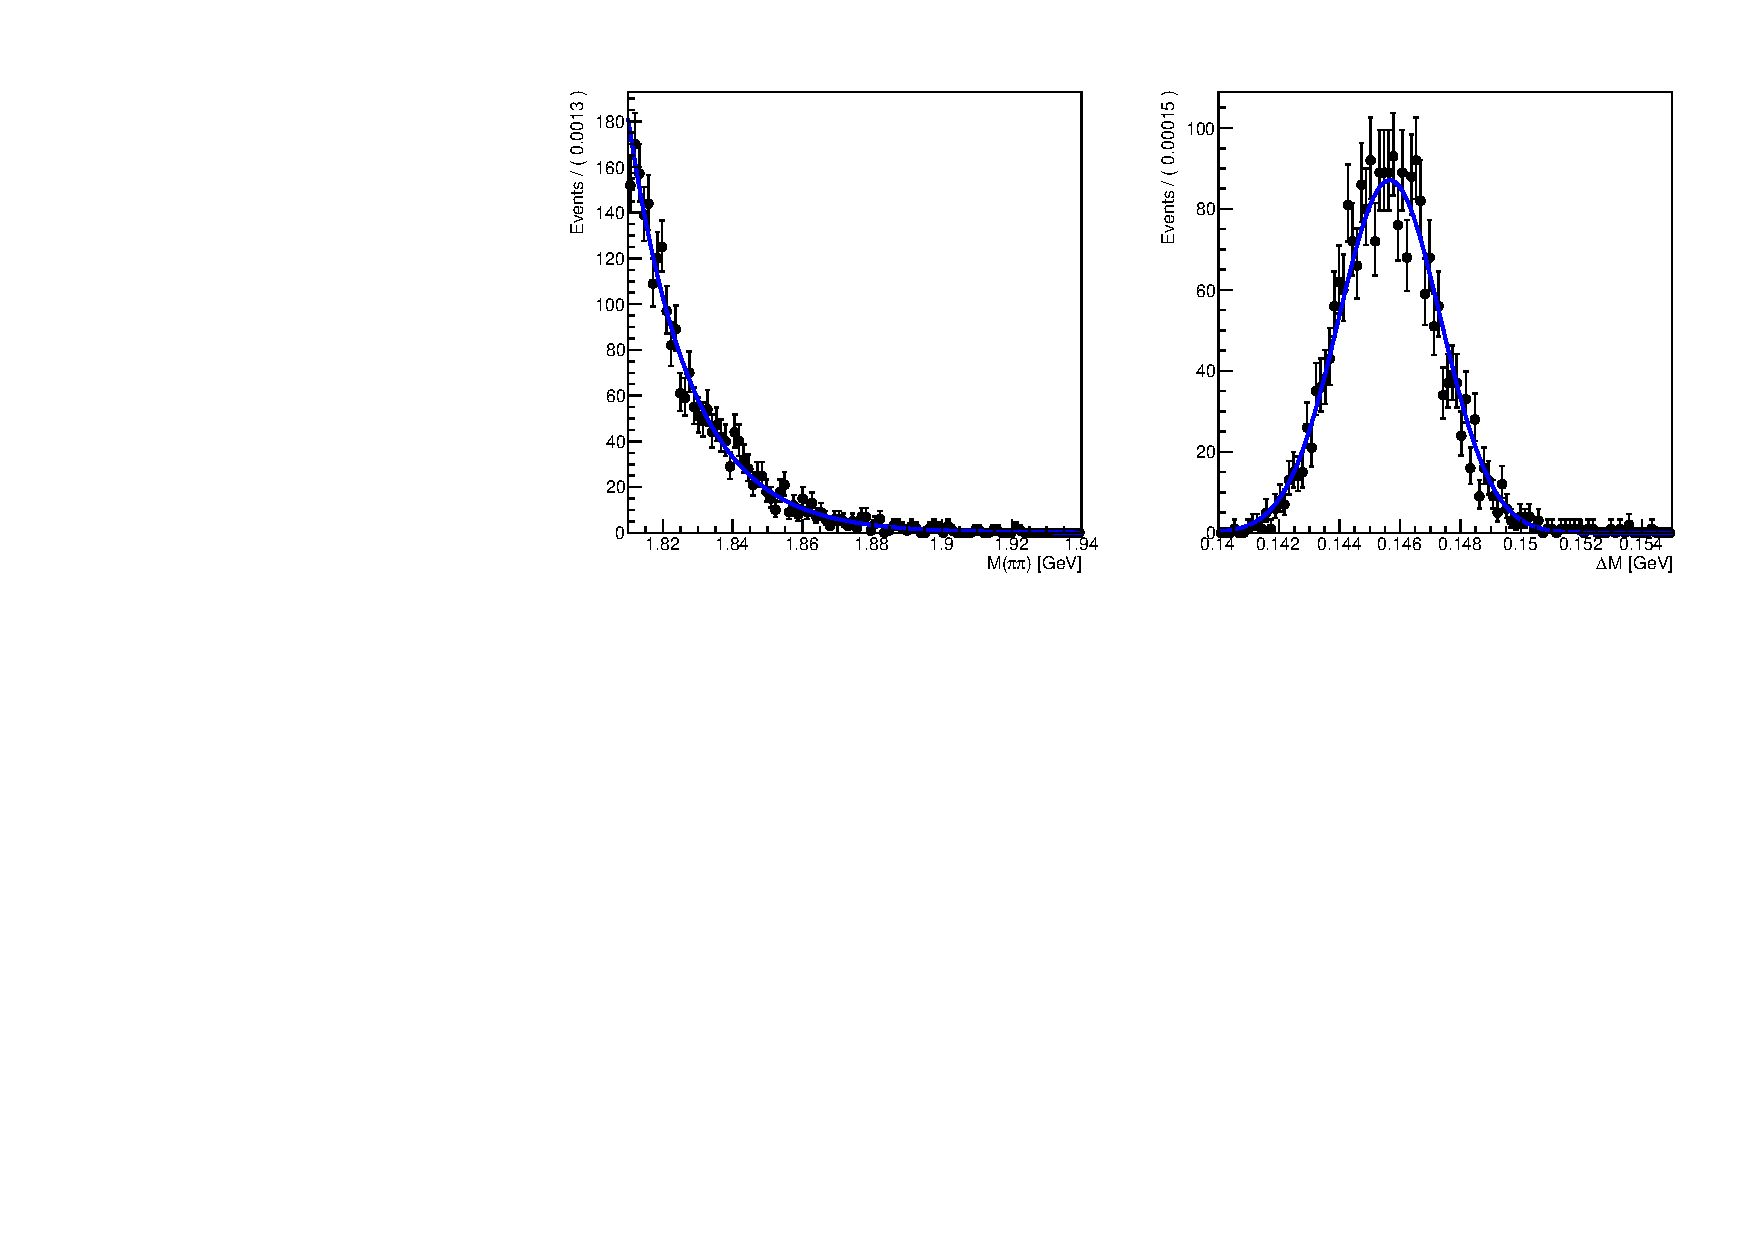
\includegraphics[width=0.9\textwidth]{figures/chapter4/normalization_fit/dpipi_fit_mc_kpi.pdf}
    \end{center}
    \caption{
      The $D^{*\pm} \to D^0\pi^\pm, D^0 \to K^\pm \pi^\mp$ model fit on MC samples, with $m(D^0)$ displayed left and $\Delta m$ displayed right.
    }
    \label{fig:d0pipi_uml_fit_kpi_model}
\end{figure}

The other two peaking backgrounds correspond to $D^0 \to \mu^+ \mu^-$ and $D^0 \to K^\pm \pi^\mp$ decays where the $D^0$ meson does not originate from a $D^*$ meson. Importantly, these have the same $m(D^0)$ shape as their $D^{*\pm} \to D^0 \pi^\pm$ counterparts, so the shape derived from their counterparts is copied exactly into their models. The $\Delta m$ of these decays, however, does not represent a peak but rather a combinatorial signature. This is due to the combinatorial nature of the production mechanisms of the $D^0$ meson that pass the selection criterion. Therefore, we fit a combinatorial background model for the $\Delta m$ values of both non-$D^{*\pm} \to D^0 \pi^\pm$ decays. 

The combinatorial background for $m(D^0)$ is an exponential function, as is common for modeling combinatorial backgrounds of reconstructed rest masses. The combinatorial background for $\Delta m$, however, has more complex shape than just an exponential. In this work, we use the $\texttt{RooDstD0Bg}$ function \cite{ref:verkerke2003roofit} given by
\begin{equation}
    P(m|m_0, A, B, C) = \left(1 - \exp \left(-\frac{m-m_0}{C} \right) \right) \left( \frac{m}{m_0}\right)^A
\end{equation}
The shape of these functions is derived from fits to the data side-band regions where the distance from the signal resonance guarantees virtually no peaking background contribution. This shape is frozen to allow for fit stability when the model is used in the final data fit. Figure \ref{fig:d0pipi_uml_fit_comb_model} shows the convergence of the shape on the data side-bands.

\begin{figure}[htp]
    \begin{center}
      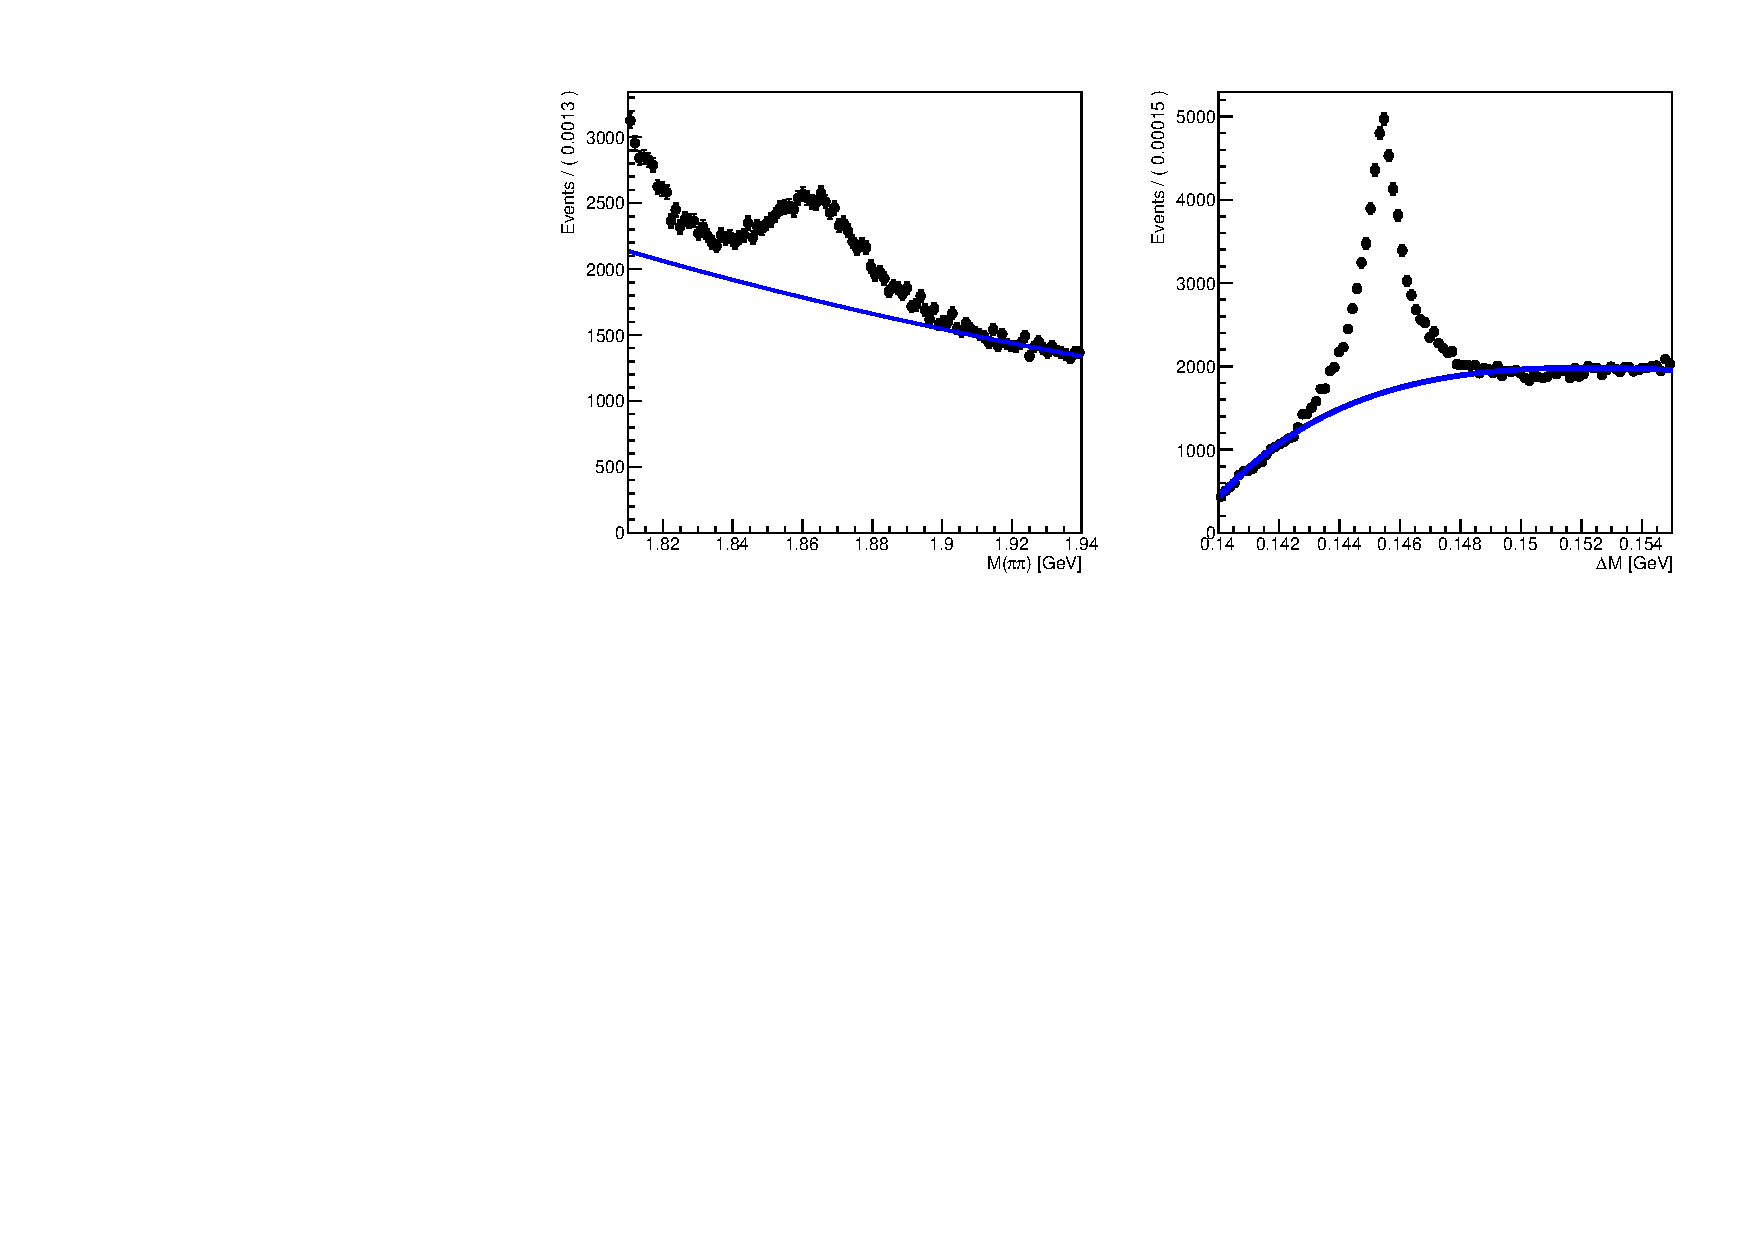
\includegraphics[width=0.9\textwidth]{figures/chapter4/normalization_fit/dpipi_fit_comb.pdf}
    \end{center}
    \caption{
      The combinatorial model fit on data side-bands, with $m(D^0)$ displayed left and $\Delta m$ displayed right.
    }
    \label{fig:d0pipi_uml_fit_comb_model}
\end{figure}

\subsubsection{Fit Results}

The final model used for the fit is a sum of signal model and all the background models. We check the convergence of this model on the \texttt{HLT\_DoubleMu4\_3\_LowMass} data, which contains significantly more signal events than the \texttt{HLT\_ZeroBias} trigger samples, allowing us to visually inspect the stability of the fit, as is seen in figure \ref{fig:d0pipi_uml_fit_dimuon} and table \ref{tab:d0pipi_uml_fit_results}. Importantly, the $D^0 \to K^\pm \pi^\mp$ decays where the $D^0$ meson does not originate from a $D^*$ meson contibutes virtually no events to the fit. Therefore, to increase the stability of the fit, we force the integral under this the non-$D^*,D^0 \to K^\pm \pi^\mp$ model to 0. 

Finally, the fit is applied to the \texttt{HLT\_ZeroBias} trigger samples. A graphical representation of the fit can be seen in figure \ref{fig:d0pipi_uml_fit} and the results are summarized in table \ref{tab:d0pipi_uml_fit_results}.


\begin{figure}[htp]
    \begin{center}
      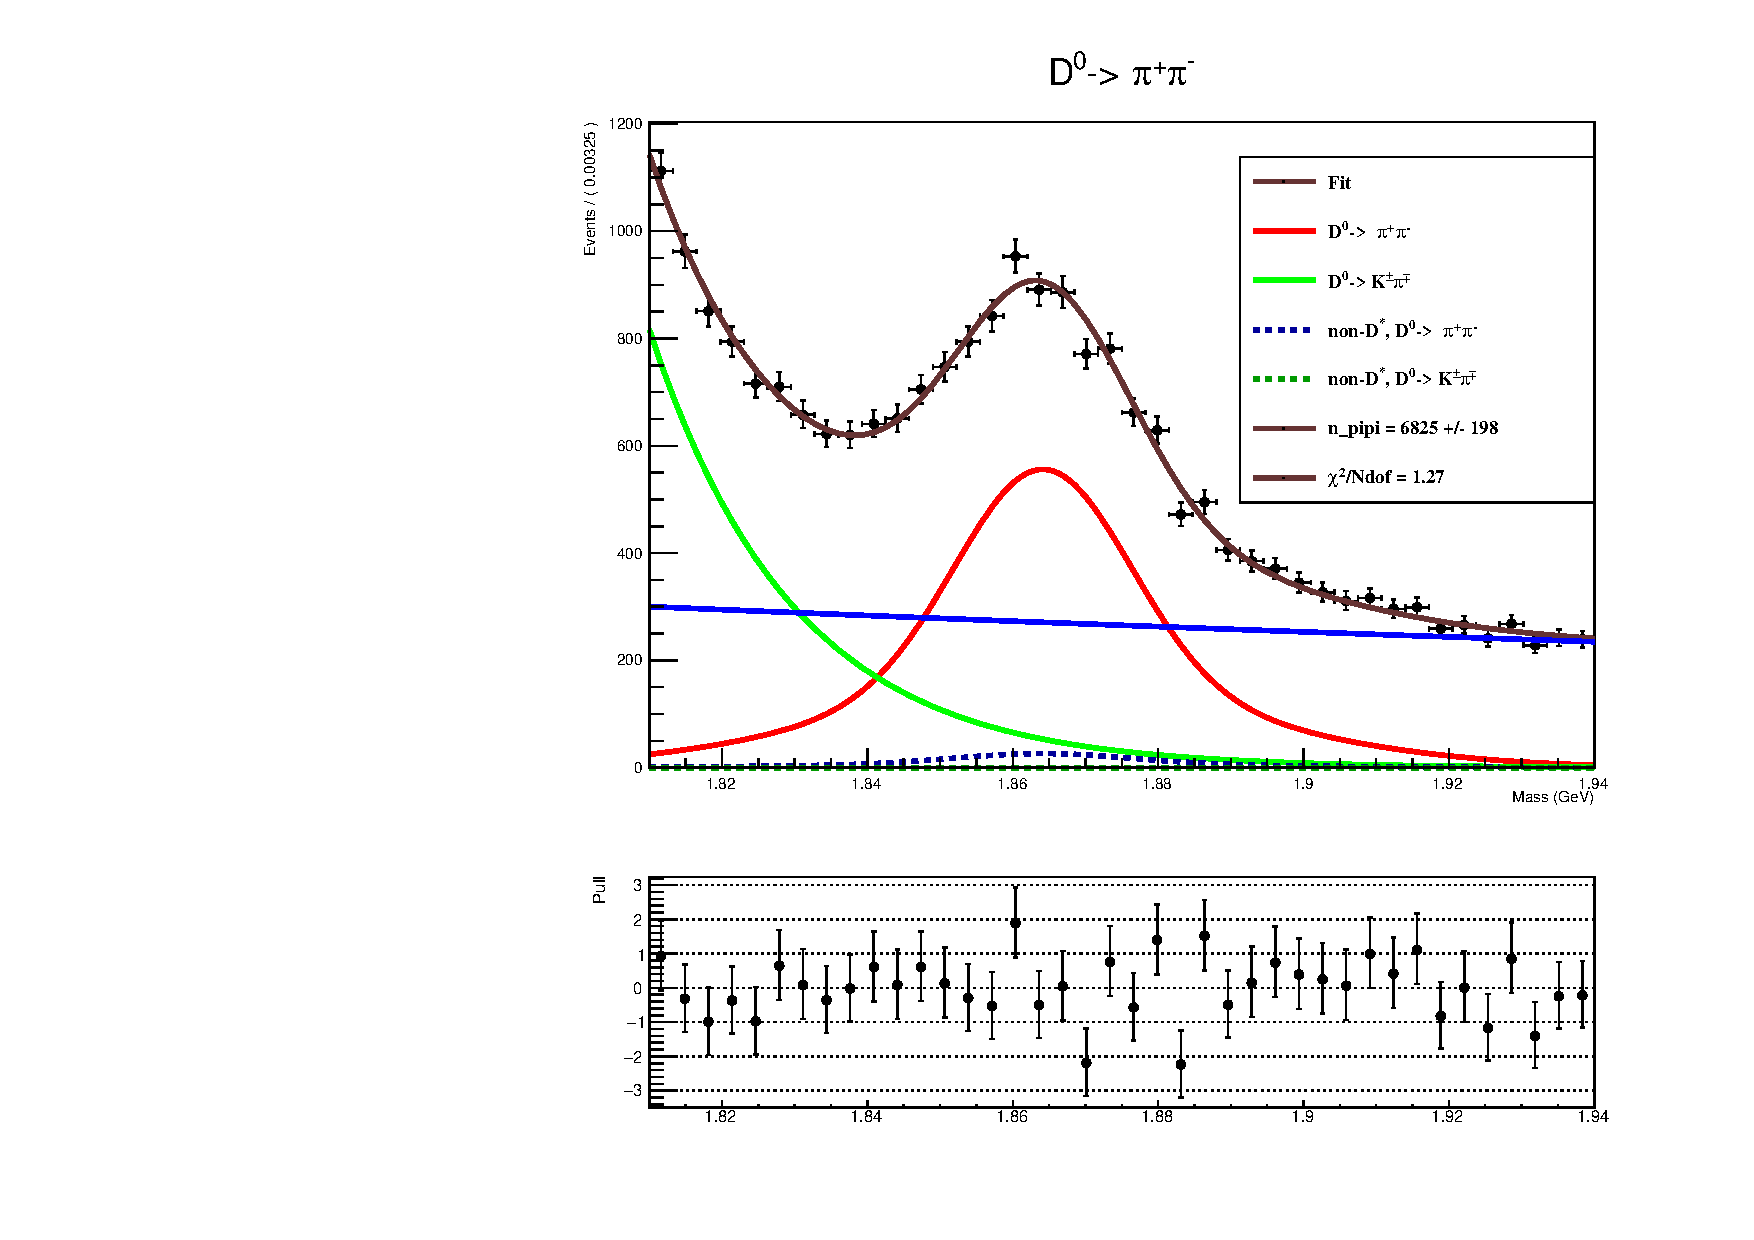
\includegraphics[width=0.45\textwidth]{figures/chapter4/normalization_fit/m_pipiDimuon_afterMvaCut.pdf}
      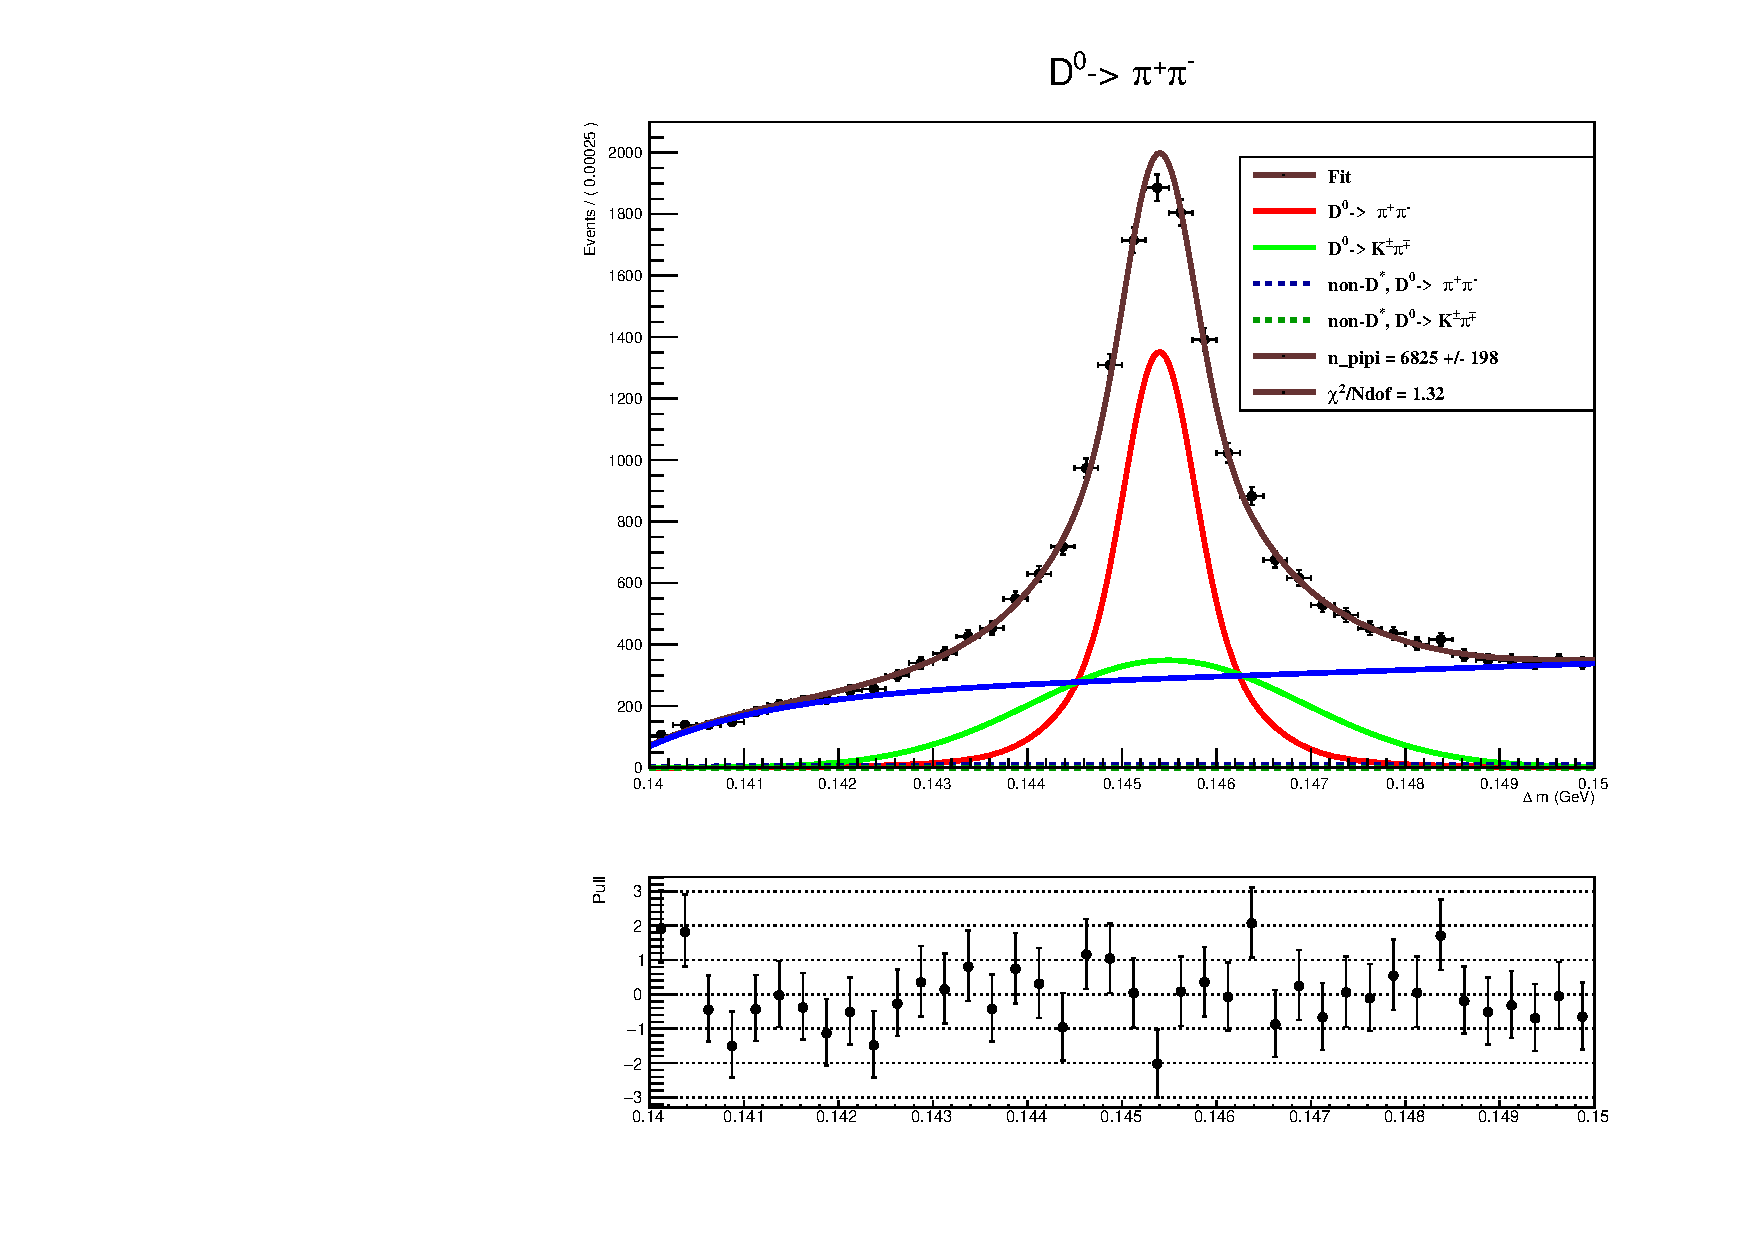
\includegraphics[width=0.45\textwidth]{figures/chapter4/normalization_fit/dm_pipiDimuon_afterMvaCut.pdf}\\
    \end{center}
    \caption{
        The full $D^0 \to \pi^+ \pi^-$ model fit on \texttt{HLT\_ZeroBias} data, with $m(D^0)$ displayed left and $\Delta m$ displayed right.
    }
    \label{fig:d0pipi_uml_fit}
\end{figure}

\begin{figure}[htp]
    \begin{center}
      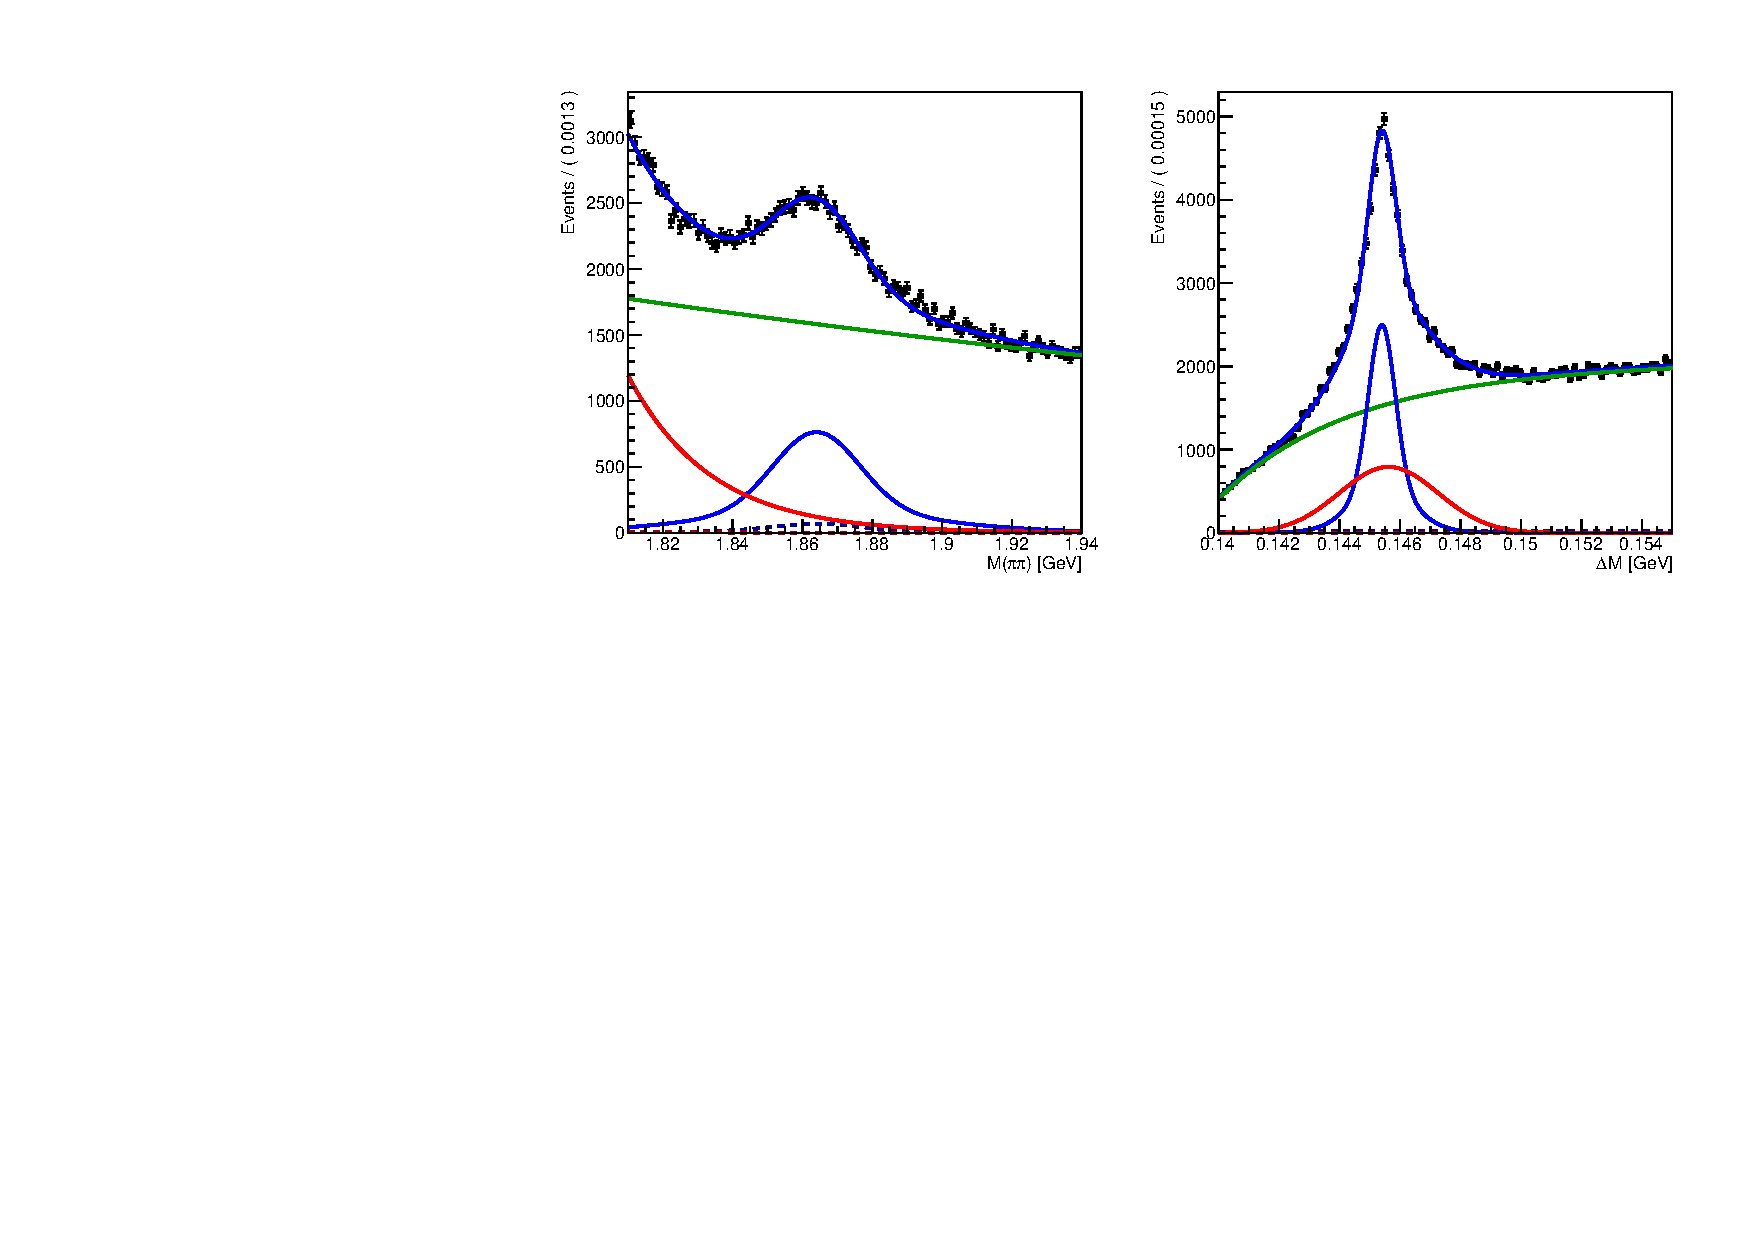
\includegraphics[width=0.9\textwidth]{figures/chapter4/normalization_fit/dpipi_fit.pdf}
    \end{center}
    \caption{
      The full $D^0 \to \pi^+ \pi^-$ model fit on \texttt{HLT\_DoubleMu4\_3\_LowMass} data, with $m(D^0)$ displayed left and $\Delta m$ displayed right. The green line follows the combinatorial model, the blue line follows the signal model, the red line follows the $D^{*\pm} \to D^0\pi^\pm, D^0 \to K^\pm \pi^\mp$ background model, the red dashed line following the non-$D^{*\pm} \to D^0\pi^\pm, D^0 \to K^\pm \pi^\mp$ background model, and the blue dashed line follows the non-$D^{*\pm} \to D^0\pi^\pm, D^0 \to \pi^+ \pi^-$ background model.
    }
    \label{fig:d0pipi_uml_fit_dimuon}
\end{figure}


\begin{table}[h!]
    \centering
    \begin{tabular}{@{}lrr@{}}
    \toprule
    \toprule
    \textbf{\texttt{HLT\_DoubleMu4\_3\_LowMass} data}& Fitted count & Fitted error  \\
    \midrule
    $D^*, D^0 \to \pi\pi$ Yield        & 23787 & $\pm$509 \\
    $D^*, D^0 \to K\pi$ Yield          & 21558  & $\pm$749 \\
    Combinatorial Yield               & 155088 & $\pm$1722 \\
    non--$D^*$, $D^0 \to \pi\pi$ Yield & 2140   & $\pm$685 \\
    non--$D^*$, $D^0 \to K\pi$ Yield   & 181     & $\pm$1410 \\
    \bottomrule
    \toprule
    \textbf{\texttt{HLT\_ZeroBias} data} & Fitted count & Fitted error \\
    \midrule
    $D^*, D^0 \to \pi\pi$ Yield        & 195 & $\pm$17 \\
    $D^*, D^0 \to K\pi$ Yield          & 74  & $\pm$21 \\
    Combinatorial Yield               & 140 & $\pm$20 \\
    non--$D^*$, $D^0 \to \pi\pi$ Yield & 0   & $\pm$11 \\
    non--$D^*$, $D^0 \to K\pi$ Yield   & 0     & $\pm$0 \\
    \bottomrule
    \bottomrule
    \end{tabular}
    \caption{Fitted yields and associated uncertainties for the normalization UML fit.}
    \label{tab:d0pipi_uml_fit_results}
    \end{table}

\subsection{Signal Channel Fit}
\label{subsec:signal_channel_uml}

The goal of the signal channel is to extract $N_{D^0 \to \mu^+ \mu^-}$. This is done using the \texttt{HLT\_DoubleMu4\_3\_LowMass} trigger dataset, as is described in section \ref{subsec:backgrounds}. As with the normalization channel, the largest difficult of this UML fit is the lack of signal events due to the small branching fraction of the $D^0$ meson. Similarly to the normalization channel, the signal channel uses MC samples to inform the shapes for data, applying corrections when needed. Additionally, the results of the normalization channel are used to fix the background yields. These techniques are described in the remaineder of the section.

It is worth mentioning that much of the machinery needed for this fit has been developed in section \ref{subsec:normalization_channel_fit} and is therefore not repeated here. Namely, this section focuses on the differences in the signal channel that require special attention.

\subsubsection{Signal Model}

The signal model for the normalization channel describes the $\Delta m$ and $m(D^0)$ of the $D^{*\pm}\to D^0 \pi^\pm, D^0 \to \pi^+ \pi^-$ decay. The same procedure for determining the normalization channel signal model is used in determining this signal model, with the mean and width corrections derived from the normalization channel.

The signal model fit to MC can be seen in figure \ref{fig:d0mumu_uml_fit}.

\begin{figure}[htp]
    \begin{center}
      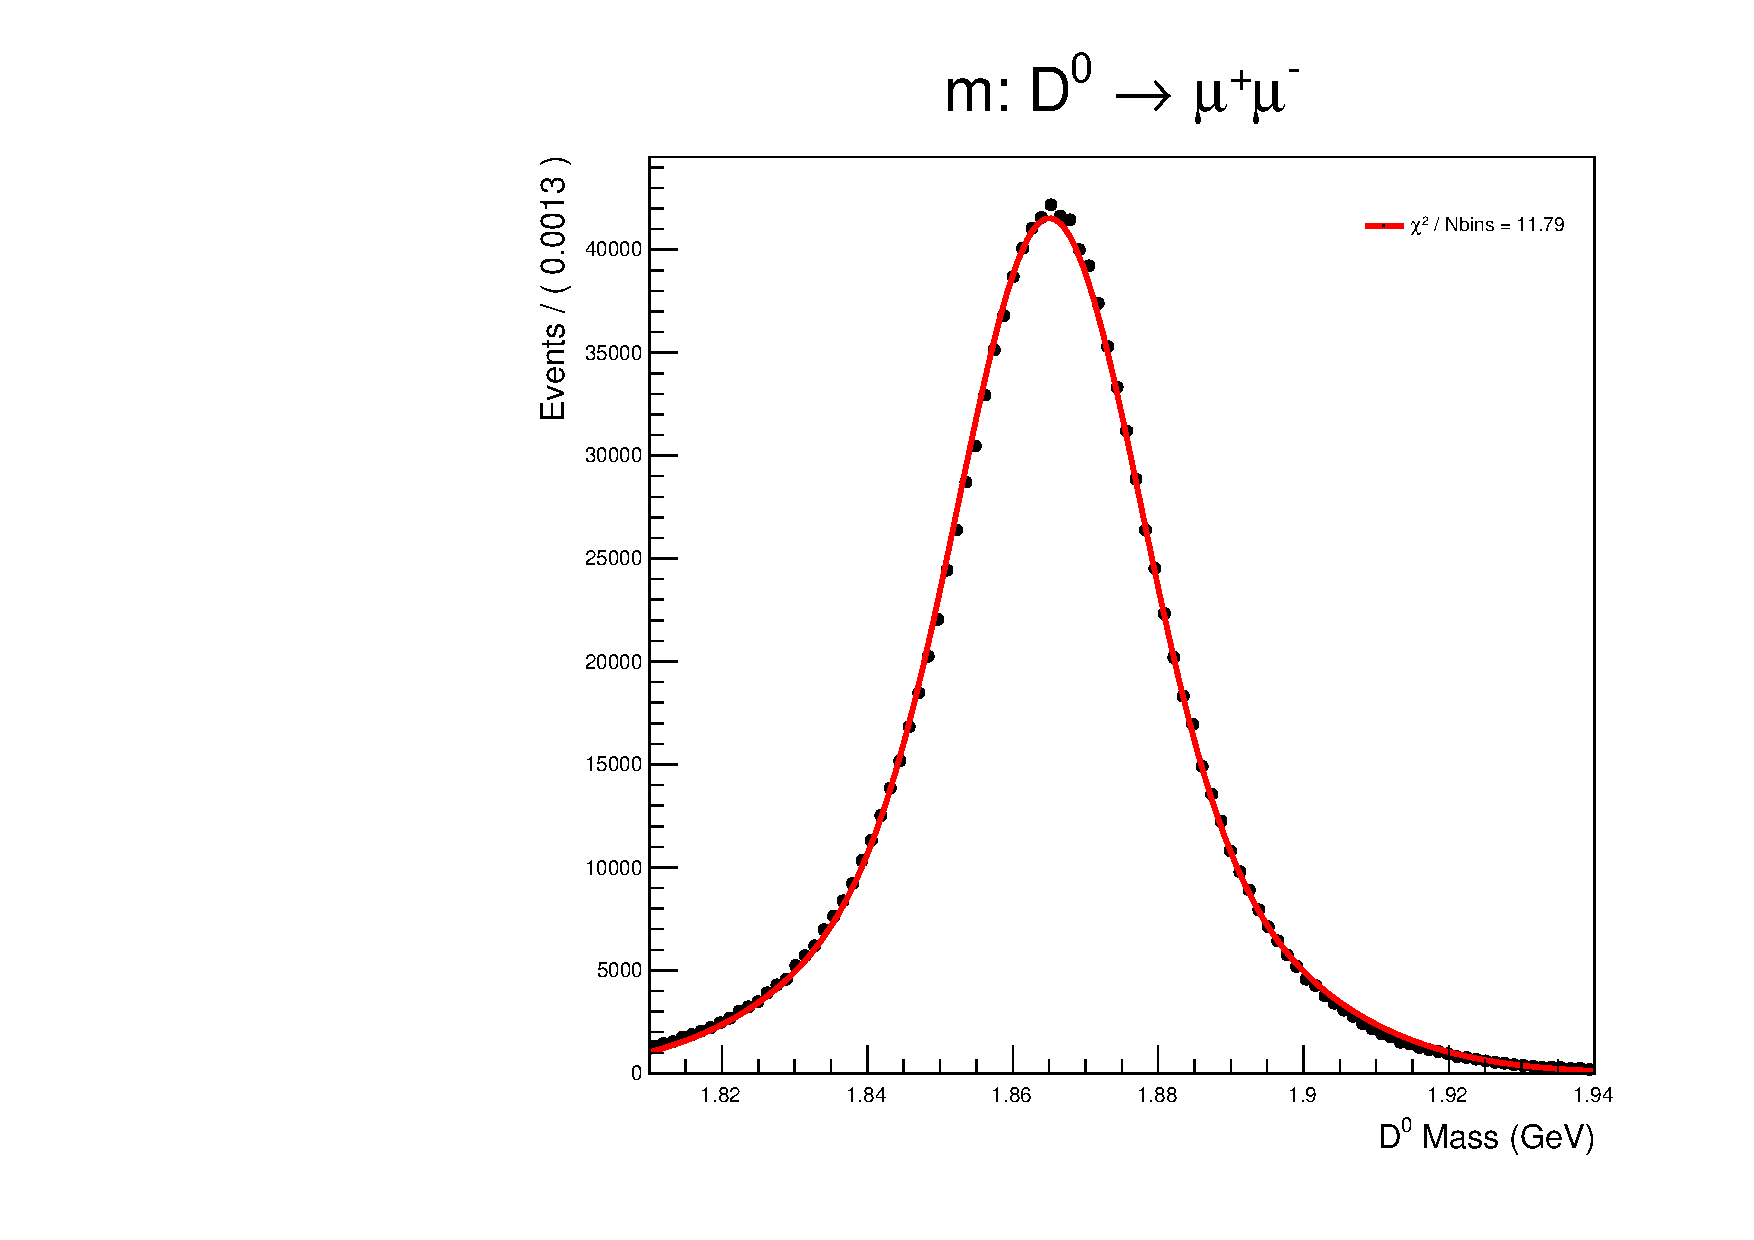
\includegraphics[width=0.45\textwidth]{figures/chapter4/signal_fit/d0mm_2022_2023_0_m.pdf}
      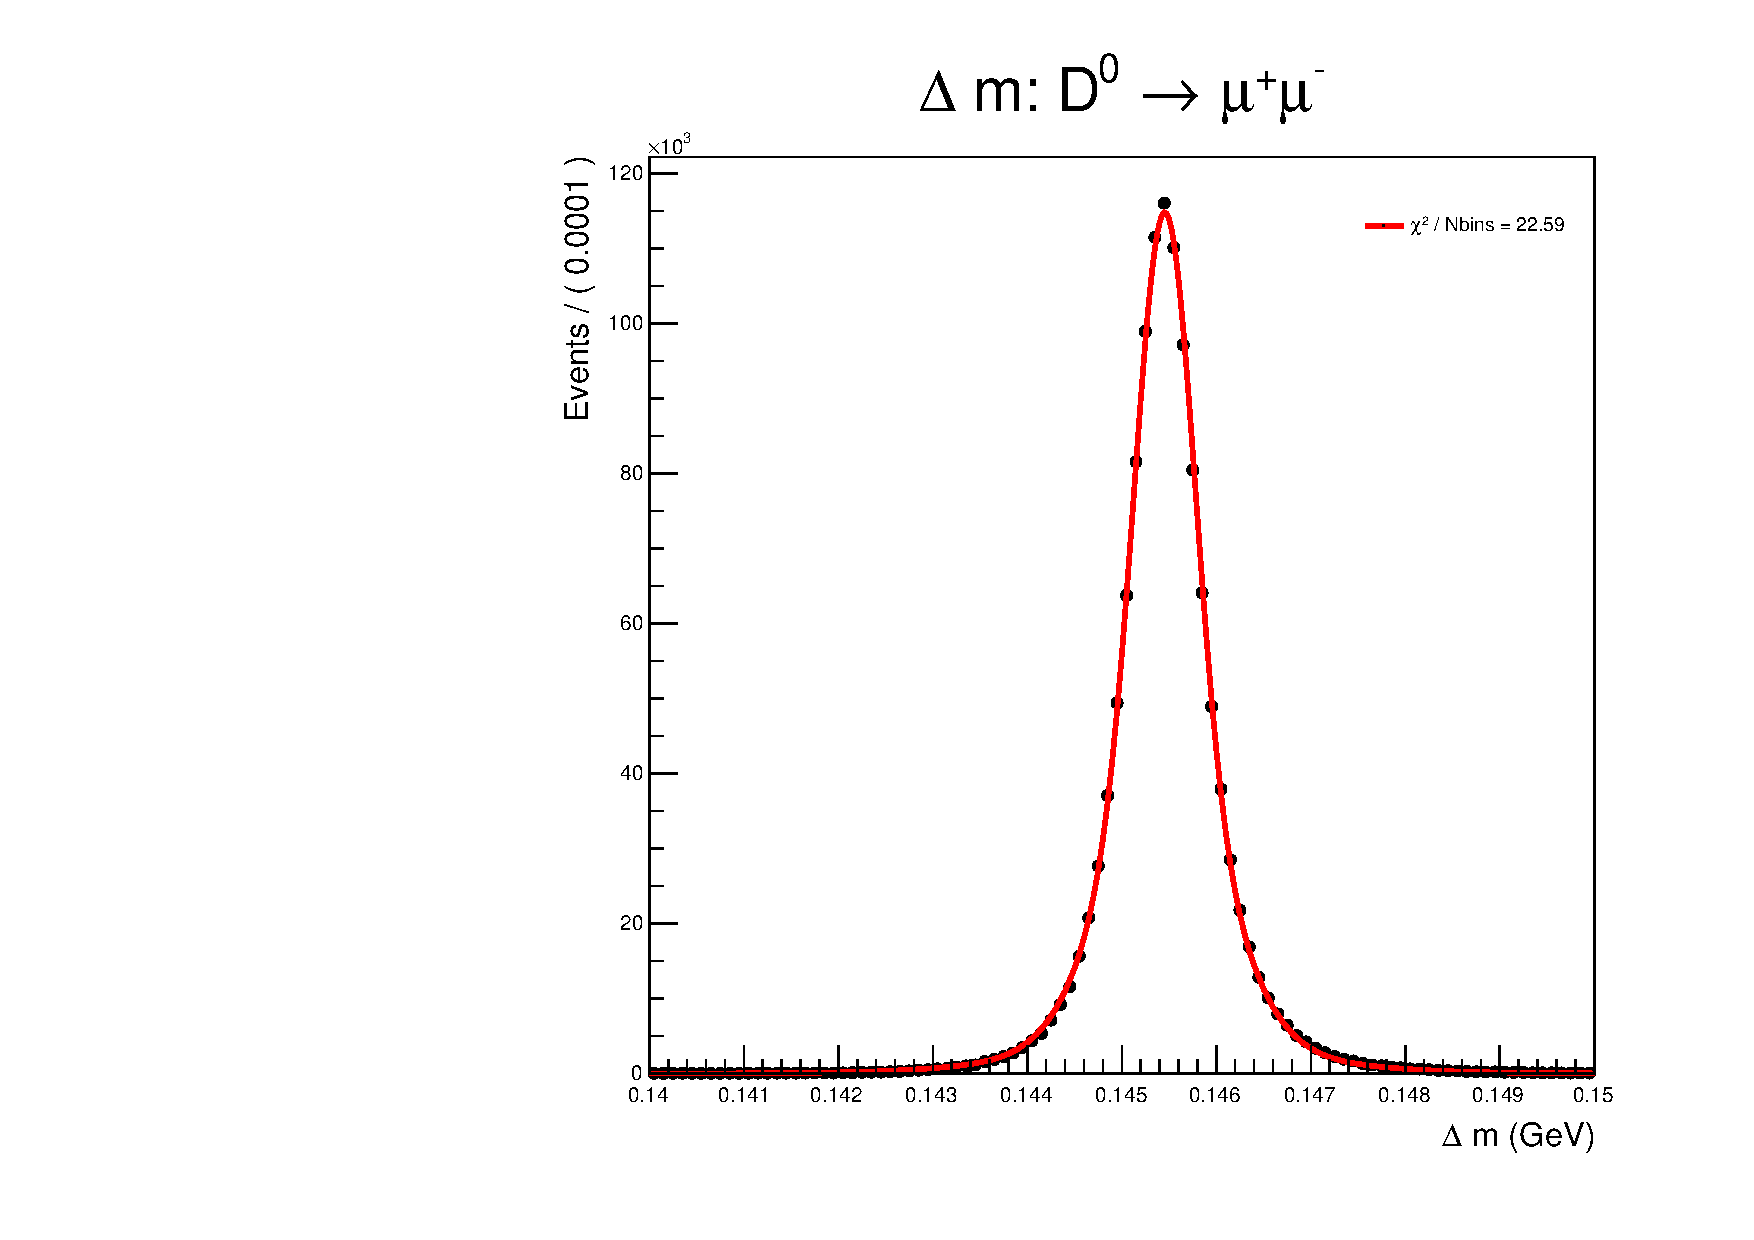
\includegraphics[width=0.45\textwidth]{figures/chapter4/signal_fit/d0mm_2022_2023_0_dm.pdf}\\
    \end{center}
    \caption{
      The signal model fit on MC samples, with $m(D^0)$ displayed left and $\Delta m$ displayed right.
    }
    \label{fig:d0mumu_uml_fit}
\end{figure}

\subsubsection{Background Model}

As is evident from section \ref{subsec:backgrounds}, there are 2 $D^{*\pm} \to D^0 \pi^\pm$ peaking backgrounds and a combinatorial background to consider in the normalization channel. Note that the non-$D^{*\pm} \to D^0 \pi^\pm$ backgrounds which were discussed extensively in the normalization channel are not relevant here due to the large uncertainty of the combinatorial background compared to the expected yield from these backgrounds. Therefore, any non-$D^{*\pm} \to D^0 \pi^\pm$ backgrounds are considered combinatorial and considered in the combinatorial model.

The two peaking backgrounds are $D^{*\pm} \to D^0 \pi^\pm$ processes where the $D^0$ decays via either $D^0 \to \pi^+ \pi^- \to \mu^+ \nu_\mu \mu^- \bar{\nu}_\mu$ (hadronic mode) or via $D^0 \to \pi^- \mu^+ \nu_\mu$ (semileptonic mode). Both of these models are developed using the same process as the signal mode. Namely, the models are built out of sums of Gaussian distributions\footnote{Just like in the signal, two Gaussian distributions sharing a common mean are used for $m(D^0)$ and three Gaussian distributions sharing a common mean are used for $\Delta m$}, their shape is determined by fitting to MC samples, and their means and widths are corrected for using the correction derived in the normalization channel fit. 

In the normalization channel, the yields of these models were left floating. In this channel, there are so few events that allowing for this would destabilize the fit. However, we have already calculated $N_{D^0 \to \pi^+ \pi^-} = 195 \pm 17$ in section \ref{subsec:normalization_channel_fit} and the branching fractions of $\mathcal{B}(D^0 \to \pi^+ \pi^-) = (1.454 \pm 0.024) \times 10^{-3}$ and $\mathcal{B}(D^0 \to \pi^-\mu^+ \nu_\mu) = (2.67 \pm 0.12) \times 10^{-3}$ are well known \cite{ref:pdg2024}. Lastly, in section \ref{sec:muon_fake_rate}, we calculate the fake rate, $f_{\pi \to \mu}$, or the rate at which pions decay to muons in the detector, which occurs once in the semi-leptonic mode and twice in the hadronic mode.

Using these qualities, as well as efficiency and MC corrections, we can write
\begin{equation}
\begin{split}
    \frac{N_{D^0 \to \pi^+ \pi^- \to \mu^+ \nu_\mu \mu^- \bar{\nu}_\mu}}{N_{D^0 \to \pi^+ \pi^-}} &= \left(f_{\pi \to \mu}\right)^2 \times \frac{\epsilon_{D^*, D^0\to\pi\pi\to\mu\mu}}{\epsilon_{D^*, D^0\to\pi\pi}} \times S_{ZB} \times \text{MVA}_D \times T_{\text{corr}} \\
    \frac{N_{D^0 \to \pi^- \mu^+ \nu_\mu}}{N_{D^0 \to \pi^+ \pi^-}} &=\frac{\mathcal{B}_{D^0 \to \pi^- \mu^ \nu_\mu}}{\mathcal{B}_{D^0 \to \pi^+ \pi^-}} \times \left(f_{\pi \to \mu}\right) \times \frac{\epsilon_{D^*, D^0\to\pi\mu\nu}}{\epsilon_{D^*, D^0\to\pi\pi}} \times S_{ZB} \times \text{MVA}_D \times T_{\text{corr}}
    \label{eq:peaking_background_yield_calculation}
\end{split}
\end{equation}
where $S_{ZB}$ is the trigger prescaling factor discussed in section $\ref{subsec:data_samples}$, $\epsilon$ is the efficiency discussed in section \ref{subsec:baseline_selection}, $\text{MVA}_D$ is the MVA correction discussed in section $\ref{subsec:mva}$, and $T_{\text{corr}}$ are the trigger corrections discussed in section \ref{subsec:trigger_efficency_correction}. The convergence of the two fits in MC is shown in figure \ref{fig:d0pimunu_uml_fit} and figure \ref{fig:d0munumunu_uml_fit}

\begin{figure}[htp]
    \begin{center}
      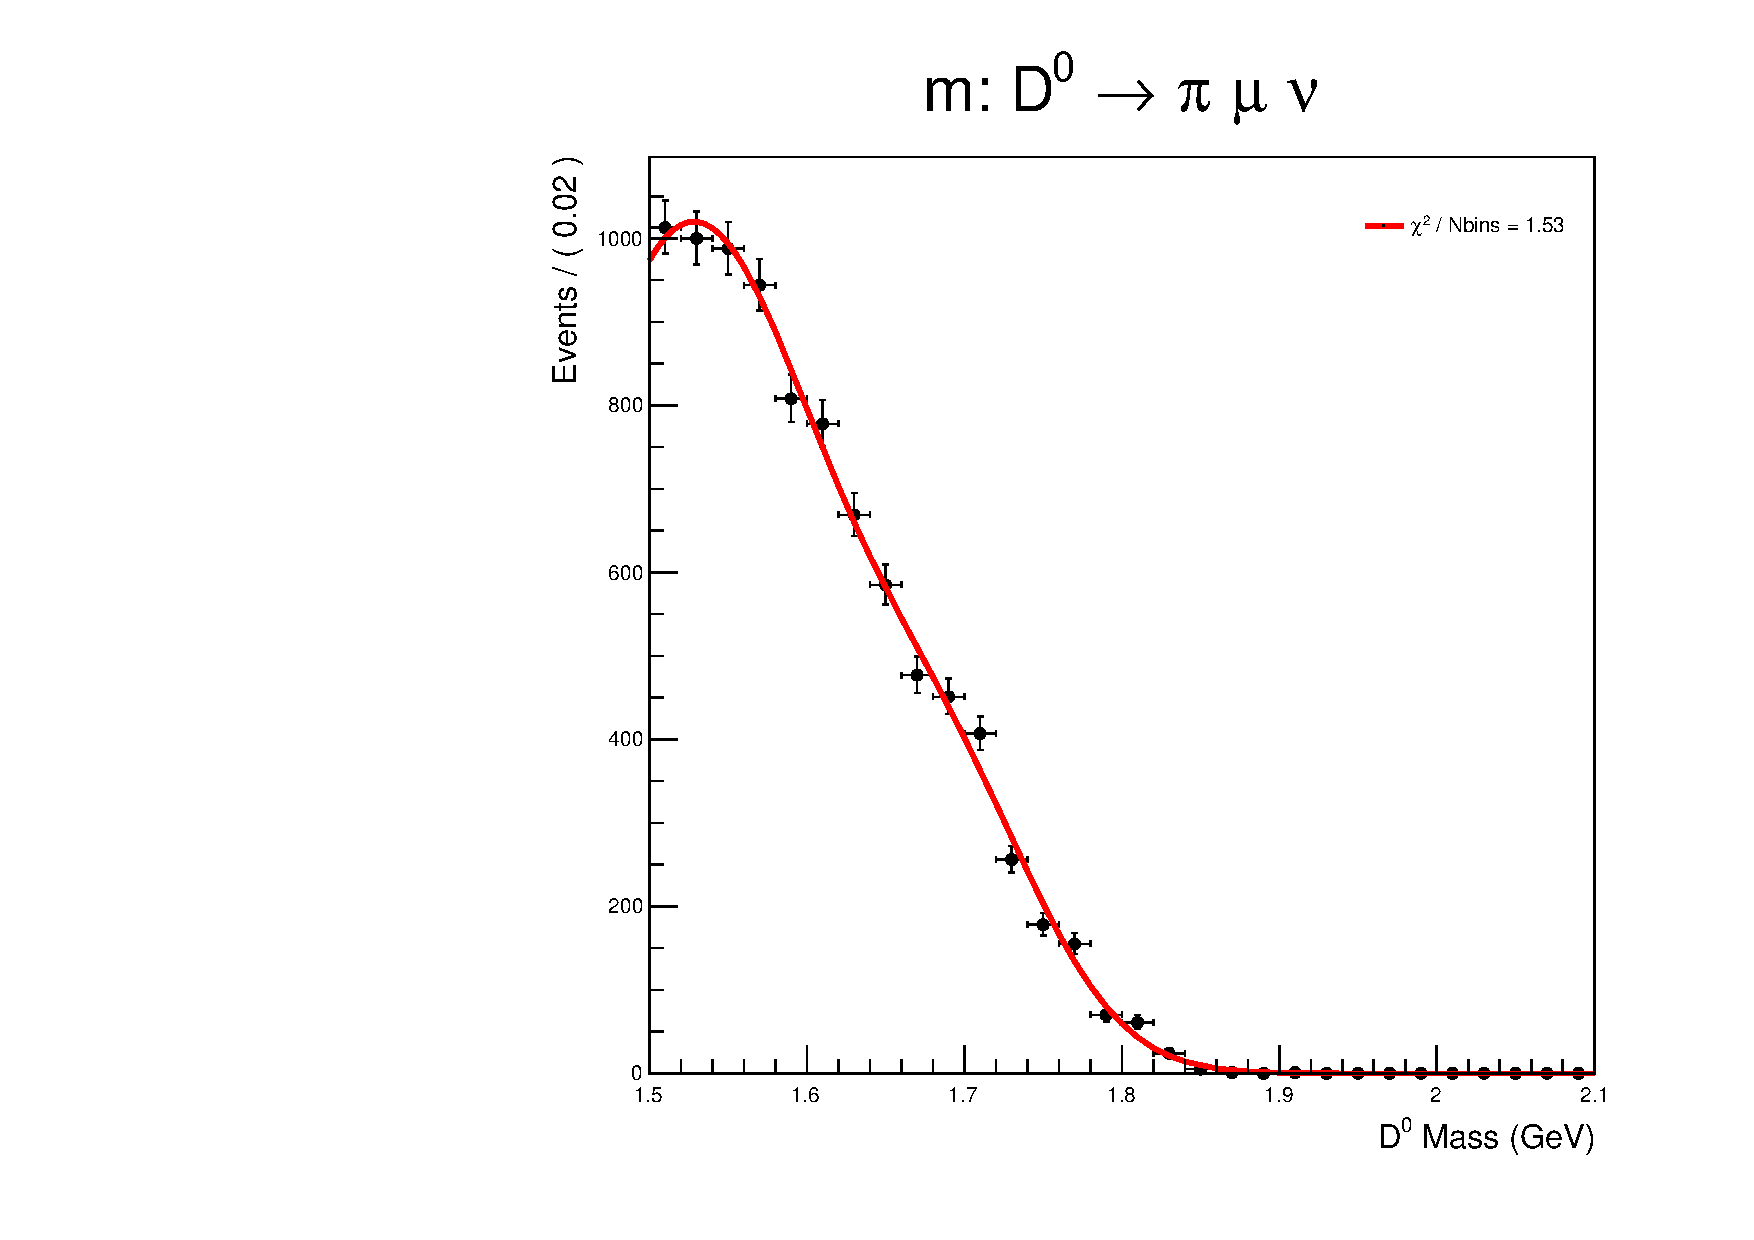
\includegraphics[width=0.45\textwidth]{figures/chapter4/signal_fit/d0pimunu_2022_2023_0_m.pdf}
      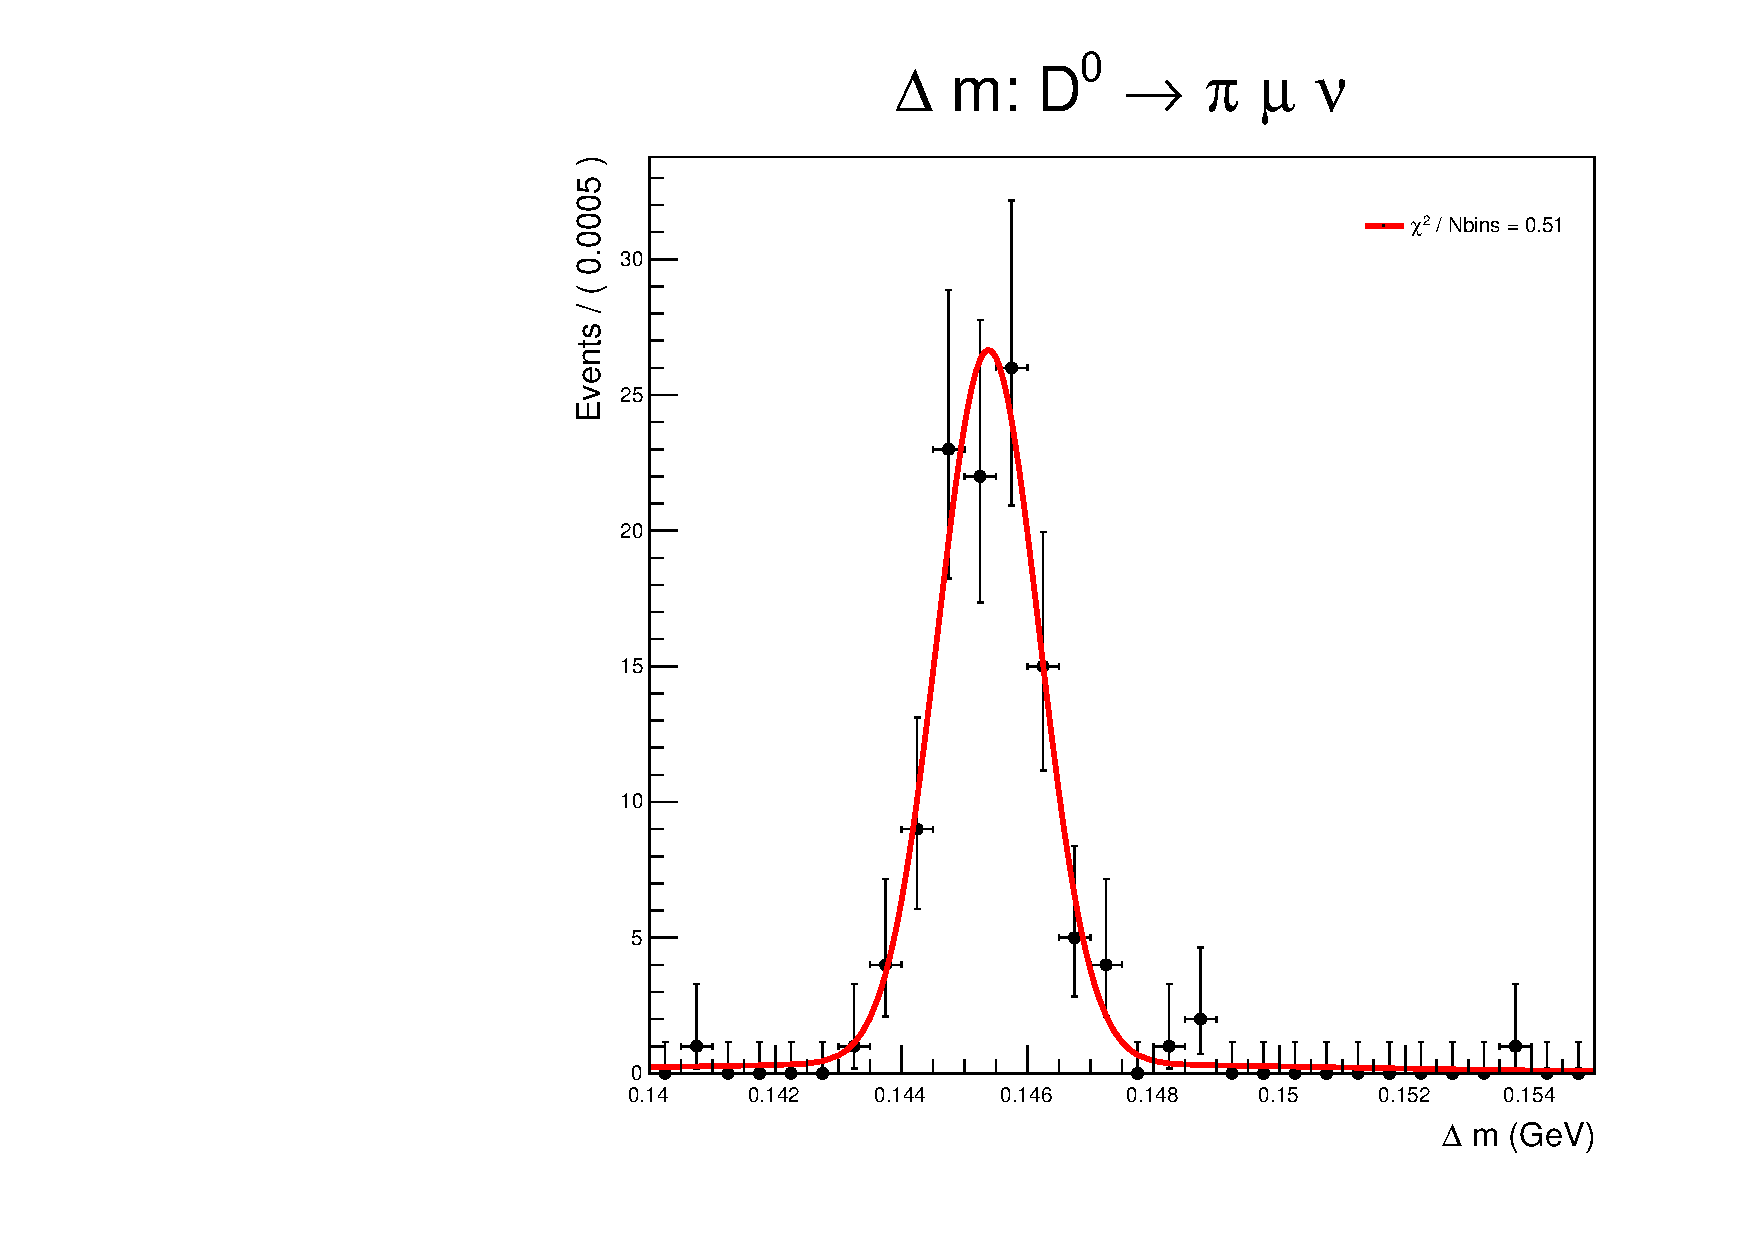
\includegraphics[width=0.45\textwidth]{figures/chapter4/signal_fit/d0pimunu_2022_2023_0_dm.pdf}\\
    \end{center}
    \caption{
      The $D^{*\pm} \to D^0\pi^\pm, D^0 \to \pi^- \mu^+ \nu_\mu$ model fit on MC samples, with $m(D^0)$ displayed left and $\Delta m$ displayed right.
    }
    \label{fig:d0pimunu_uml_fit}
\end{figure}

\begin{figure}[htp]
    \begin{center}
      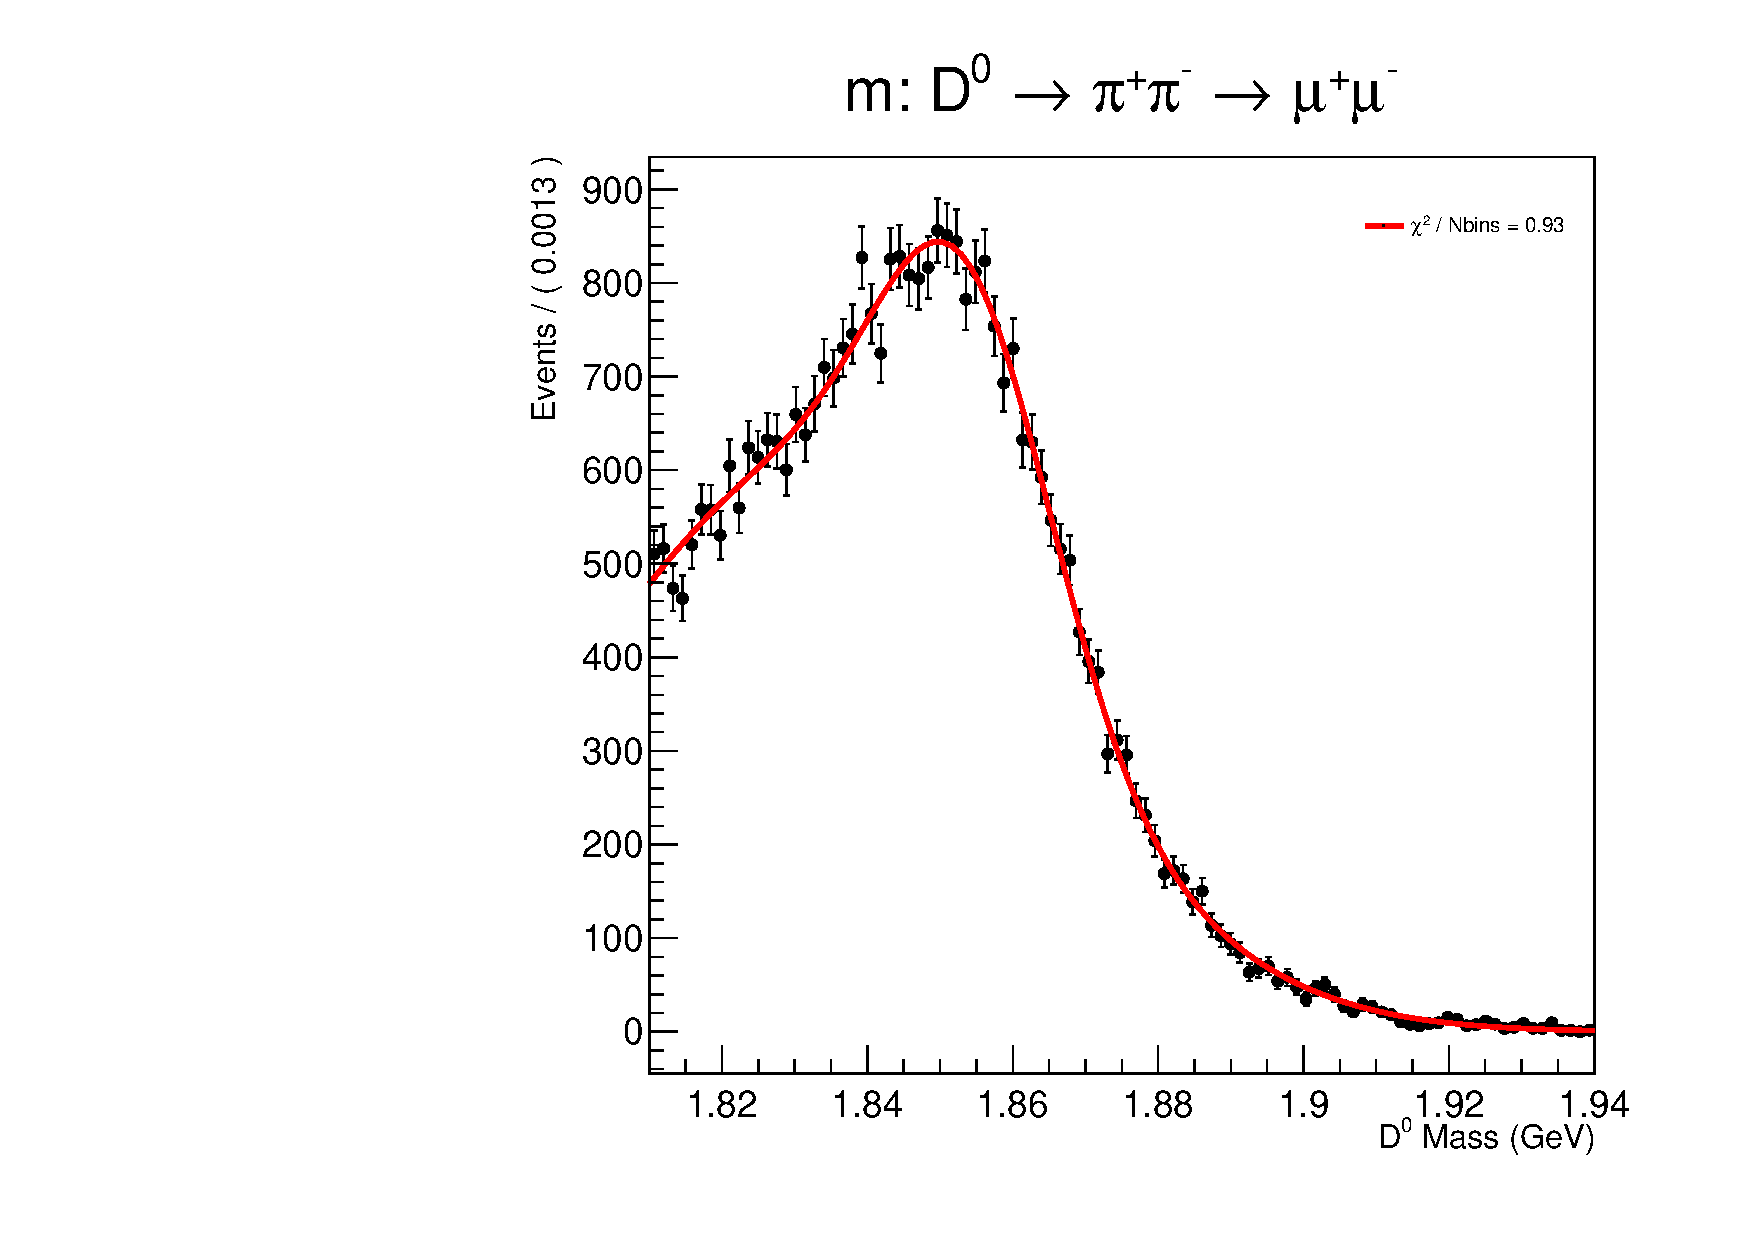
\includegraphics[width=0.45\textwidth]{figures/chapter4/signal_fit/d0pipimm_2022_2023_0_m.pdf}
      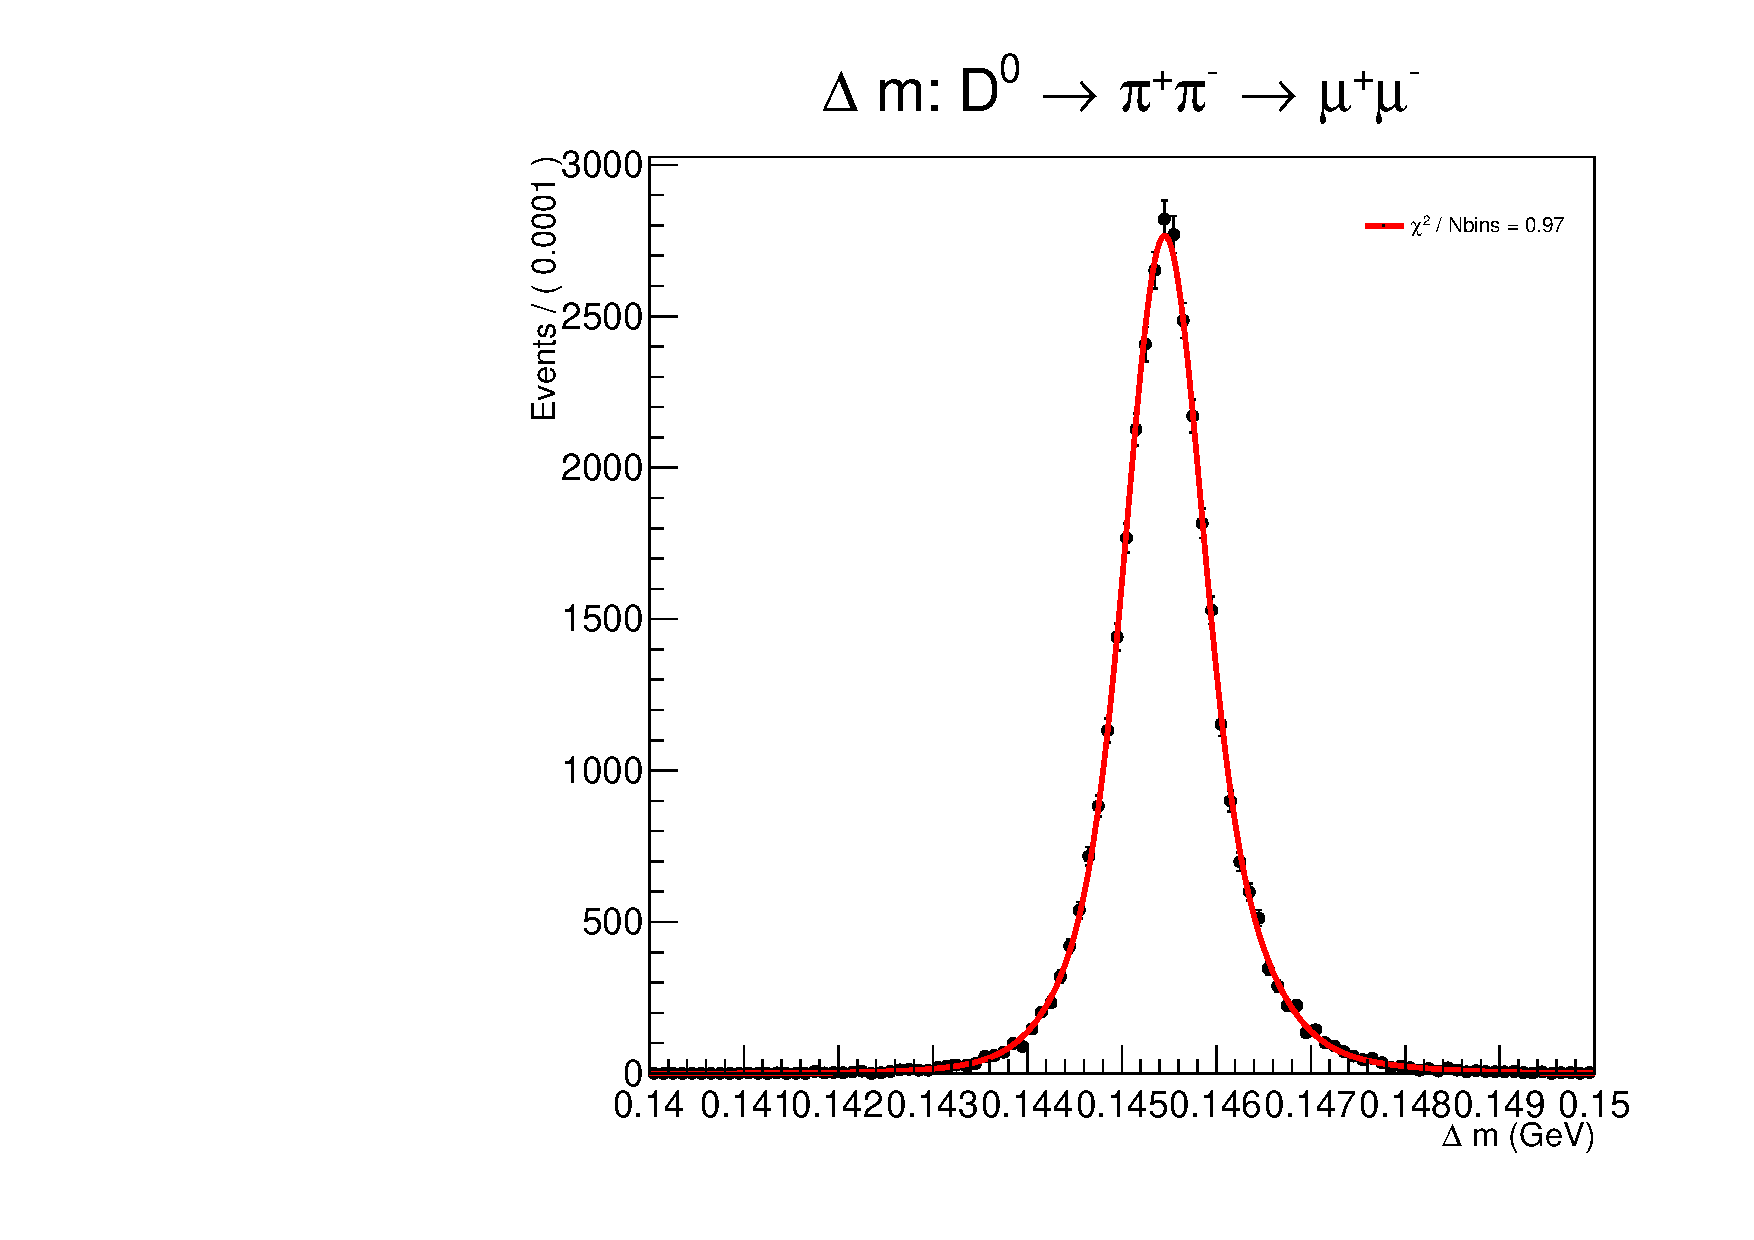
\includegraphics[width=0.45\textwidth]{figures/chapter4/signal_fit/d0pipimm_2022_2023_0_dm.pdf}\\
    \end{center}
    \caption{
      The $D^{*\pm} \to D^0\pi^\pm, D^0 \to \pi^+ \pi^- \to \mu^+ \nu_\mu \mu^- \bar{\nu}_\mu$ model fit on MC samples, with $m(D^0)$ displayed left and $\Delta m$ displayed right.
    }
    \label{fig:d0munumunu_uml_fit}
\end{figure}


The process for determining the combinatorial model is kept the same as for the normalization channel. The only difference is that due to the added complexity of the backgrounds, the $m(D^0)$ pdf function is a combination of a Bernstein polynomial, power law, and exponential function, instead of just an exponential function as was used in the normalization channel. Similar to the normalization channel, the shape and yield is determined using data side-bands, leaving no combinatorial variables left to fit in the main data region. The convergence of the combinatorial fit using partially unblinded data sidebands can be seen in figure \ref{fig:signal_comb_uml_fit}.

\begin{figure}[htp]
    \begin{center}
      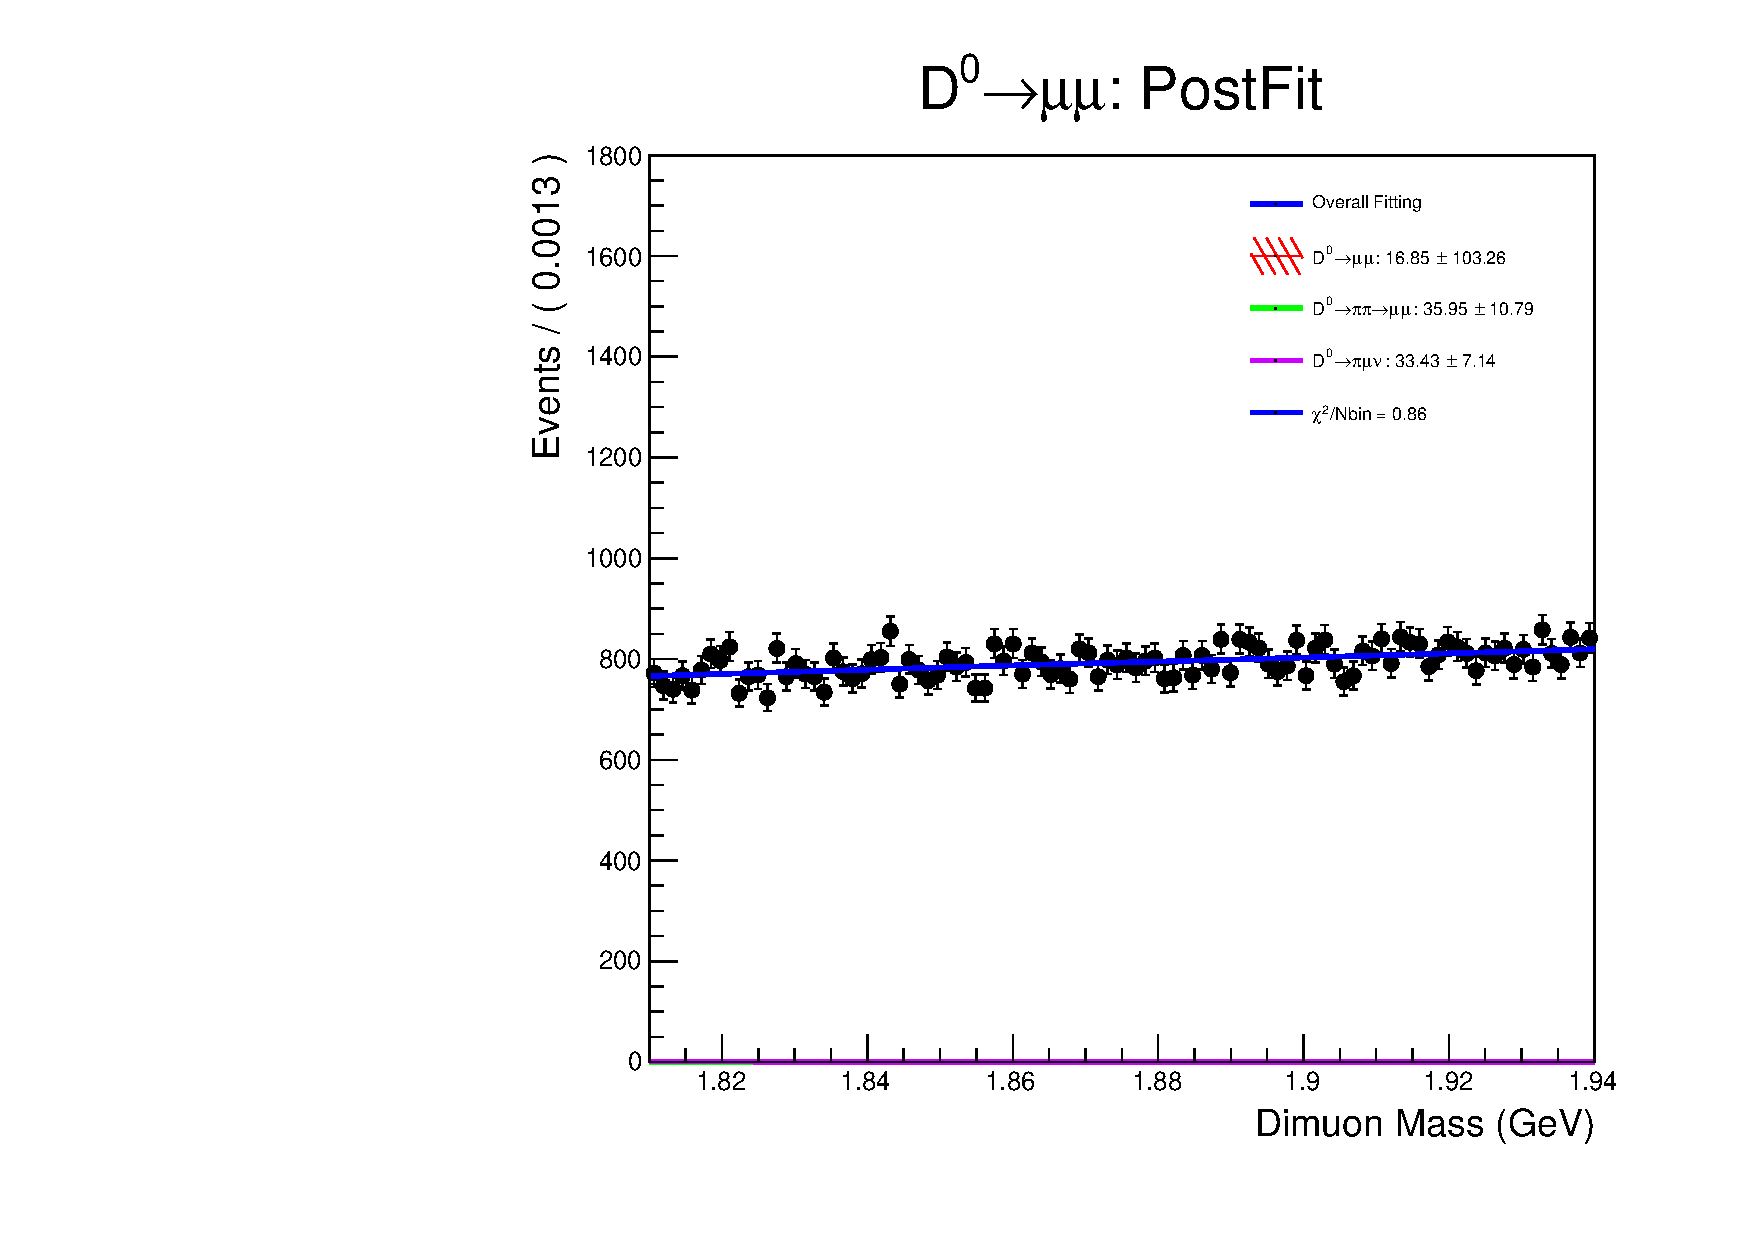
\includegraphics[width=0.45\textwidth]{figures/chapter4/signal_fit/partial_fit_m.pdf}
      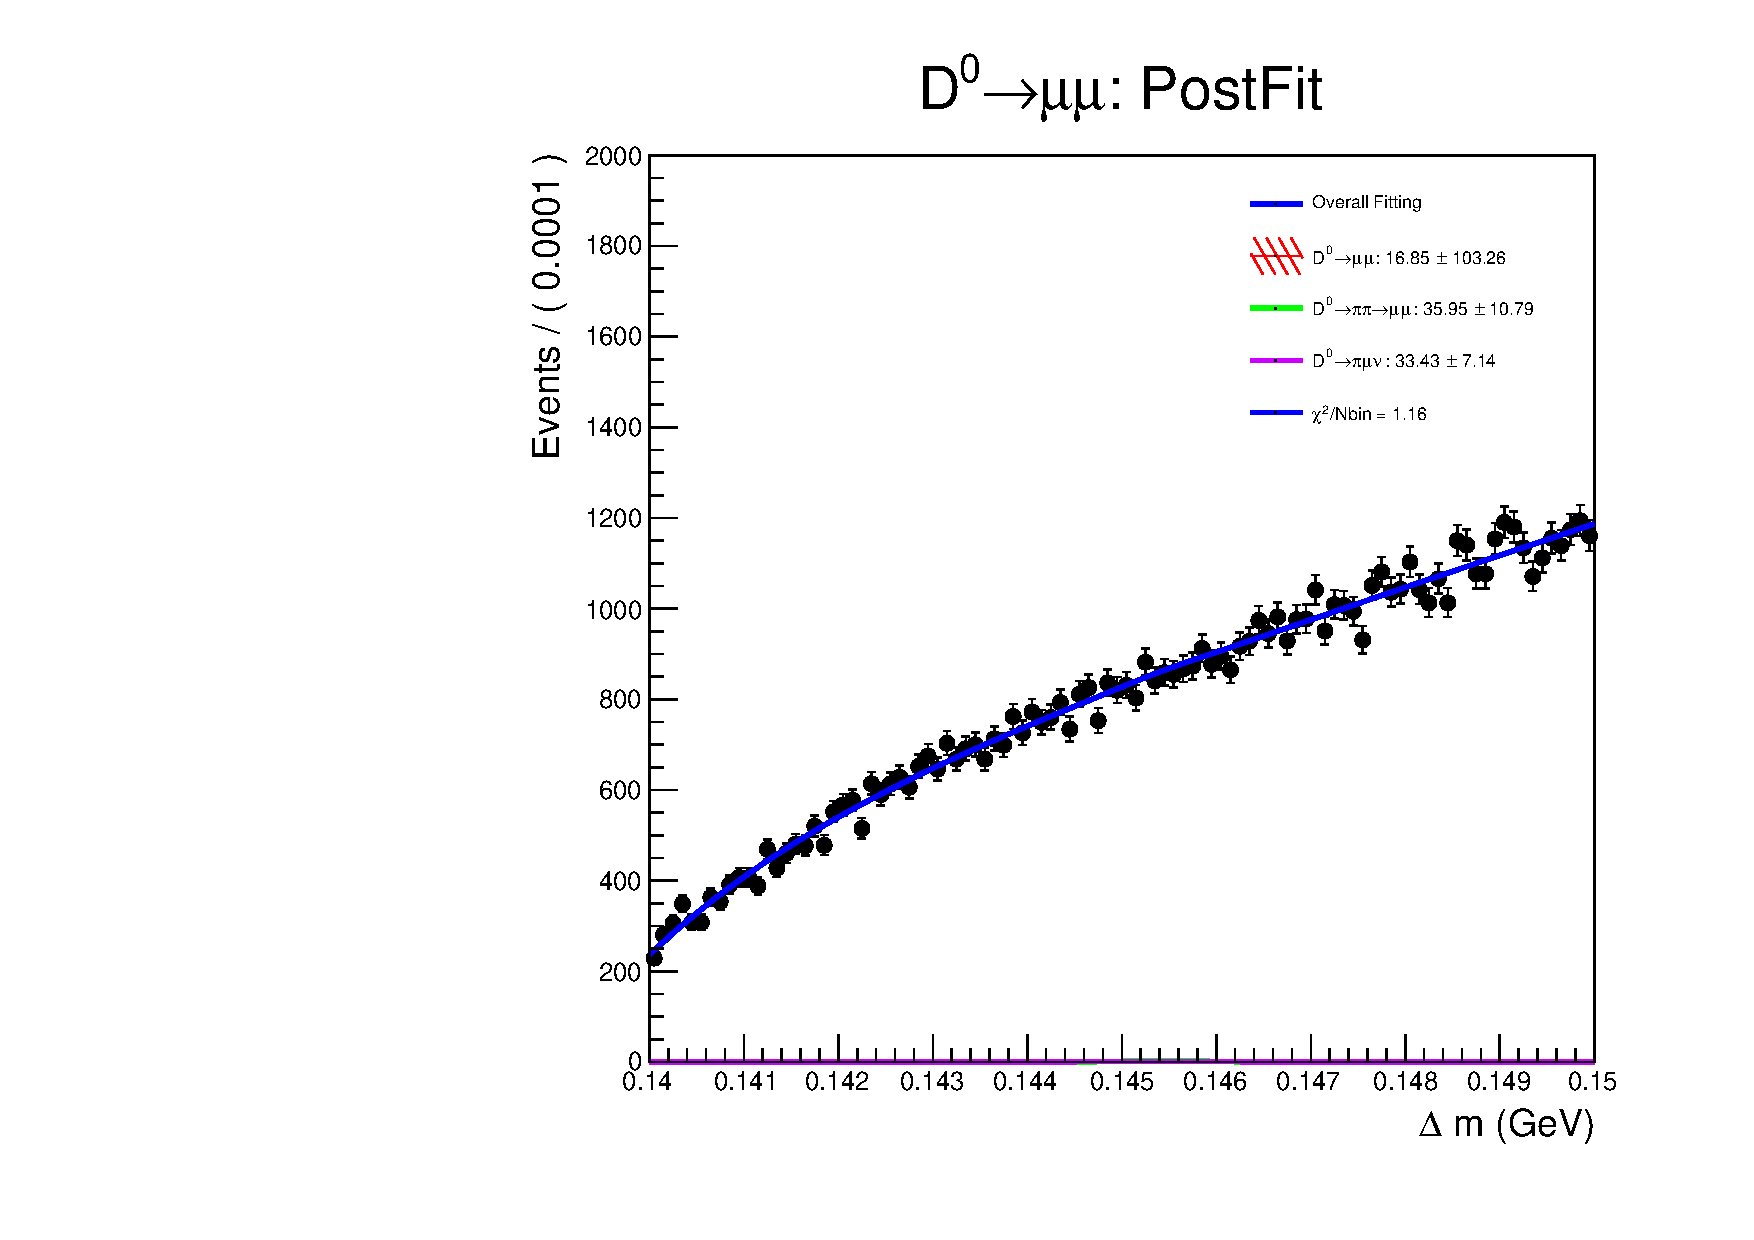
\includegraphics[width=0.45\textwidth]{figures/chapter4/signal_fit/partial_fit_dm.pdf}\\
    \end{center}
    \caption{
      The fit to partial unblinded data before any $\text{MVA}_D$ cut, demonstrating the stability of the combinatorial shape which dominates the overall shape.
    }
    \label{fig:signal_comb_uml_fit}
\end{figure}

\subsubsection{Fit Results}

The final model used for the fit is a sum of signal model and all the background models. One important note is to emphasize that the signal shape and peaking background shape are entirely deriving from MC, the peaking background yeild is determined from equation \ref{eq:peaking_background_yield_calculation}, and combinatorial background shape and yield are determined by the data side-bands. Therefore, the only parameter of this fit is the actual parameter of interest, namely the $N_{D^0 \to \pi^+ \pi^-}$ events. 

The results of this fit are only seen after unblinding the data in as discussed in section \ref{sec:analysis_overview}. The results are presented in section \ref{subsec:final_result}.

\section{Muon Fake Rates}
\label{sec:muon_fake_rate}

A muon fake occurs in this analysis when a pion decay product is measured as muon. This most commonly occurs due to in-flight pion decays, $\pi \to \mu \nu$, but can also occur due to detector misreconstruction. As a result, the more common $D^0 \to \pi^+ \pi^-$ process can mimic genuine $D^0 \to \mu^+ \mu^-$ events when the pions decay in flight, producing muons that are misidentified as signal and causing a significant challenge to this analysis. Therefore, a clear and precise understanding of the muon fake rate must be achieved to be used throughout the rest of the analysis. The below method was first developed to search for the $B^0 \to \mu^+ \mu^-$ decay \cite{ref:2023b0mumu}. Below we summarize the most relevant aspects of the procedure and results for the \texttt{Loose} muon identification system, the \texttt{highPurity} inner track quality requirements, tracker muon, and global muon requirements. These requirements reflect the selection critierion for the rest of the analysis described in section \ref{subsec:preselection} and section \ref{subsec:baseline_selection}.

\subsection{Data Samples and Selections}

To get a reliable prediction for muon fake rates we need to be able to simulate pion decays in flight. We also needed to be able to simulate reconstructing the pion as a muon candidate through a muon identification scheme. While pion decays into muons can be simulated with adequate precision in MC, the reconstruction and muon identification parts are harder to simulate correctly. Therefore, we need to be able to measure the fake rates in data, then use those results to correct MC predictions. To increase the sensitivity of the fake rate measurement, we use control samples that clearly identify hadrons in data and MC. Additionally, to avoid a dependence on the trigger, we pick samples with triggers that only fire on  electrons. Using this, we remove trigger dependence on muons, removing a trigger  bias toward muons from the sample. Thus, the data samples used is in this anaylsis are \texttt{EGamma (2022)}, \texttt{EGamma0 (2023)}, \texttt{Egamma1 (2023)}, and \texttt{ParkingDoubleElectronLowMass}. The \texttt{EGamma} datasets require events to pass single-electron triggers, while \texttt{ParkingDoubleElectronLowMass} relies on low-mass dielectron triggers with reduced prescales, enabling efficient selection of low-momentum hadronic decays.

For MC studies of muon fake rates, several background samples are used to provide a realistic modeling of processes that can produce hadrons misidentified as muons. Drell-Yan samples with dileptons and two associated jets are included, both in the low-mass (10-50 GeV) and high-mass (above 50 GeV) regimes, generated using the \texttt{amcatnloFXFX} and \texttt{madgraphMLM} frameworks interfaced with \texttt{pythia8}. A dedicated sample of Drell-Yan to dielectrons is also included to help disentangle muon-specific effects. Additionally, \texttt{$W\to l \nu$} events with jets and \texttt{t$\bar{\text{t}}$} events in the lepton+jets final state are included to capture fake muons arising in high-activity environments with real leptons and multiple jets. All samples are produced at $\sqrt{s} = 13.6$ TeV and use the \texttt{TuneCP5} parton shower configuration.

To study muon fakes originating from pions we use $K_S^0 \to \pi^+ \pi^-$ control sample. The selection requirements are:
\begin{itemize}
\item $p_{T}^{\pi_1}>1$ GeV
\item $p_{T}^{\pi_2}>4$ GeV
\item pion track is highPurity
\item $m_{K_S^0}\in[0.45,0.55]$
\item $\frac{L_{xy}}{\sigma_L}>3$
\item Vertex probability greater than 0.001
\item vertex displacement in XY plane wrt Beam Spot less than 8
\item cosine of pointing angle in XY wrt BS greater than 0.999
\item impact parameter significance of the candidate trajectory in 3D wrt PV less than 3
\item 2D impact parameter significance for Track 1 and 2 wrt Beam Spot greater than 5
\item kinematic vertex fit $\chi^{2}/dof$ of the two track less than 3
\item Fire the HLT Electron30 trigger
\end{itemize}


\subsection{Measurement Procedure}

To measure the fake rate we perform an extended binned maximum likelihood fit to
$\pi^{+}\pi^{-}$ and $\mu^{\pm}\pi^{\pm}$ invariant mass distribution to extract
the event yield of $K_S^0 \to \pi^+ \pi^-$ and $K_S^0 \to \mu^\pm \pi^\mp$ events. The model used to describe the signal and combinatorial background component are a Crystall Ball added to a  Gaussian centered at the same mean and a 2nd order Bernstein polynomial function, respectively. The signal shape in the $K_S^0 \to \mu^\pm \pi^\mp$ distribution is fixed from the $K_S^0 \to \pi^+ \pi^-$  distribution to avoid the different signal shape due to the low statistics. One of the fit projection is shown in the figure~\ref{fig:fit_example_pion}

\begin{figure}[!h]
  \begin{center}
    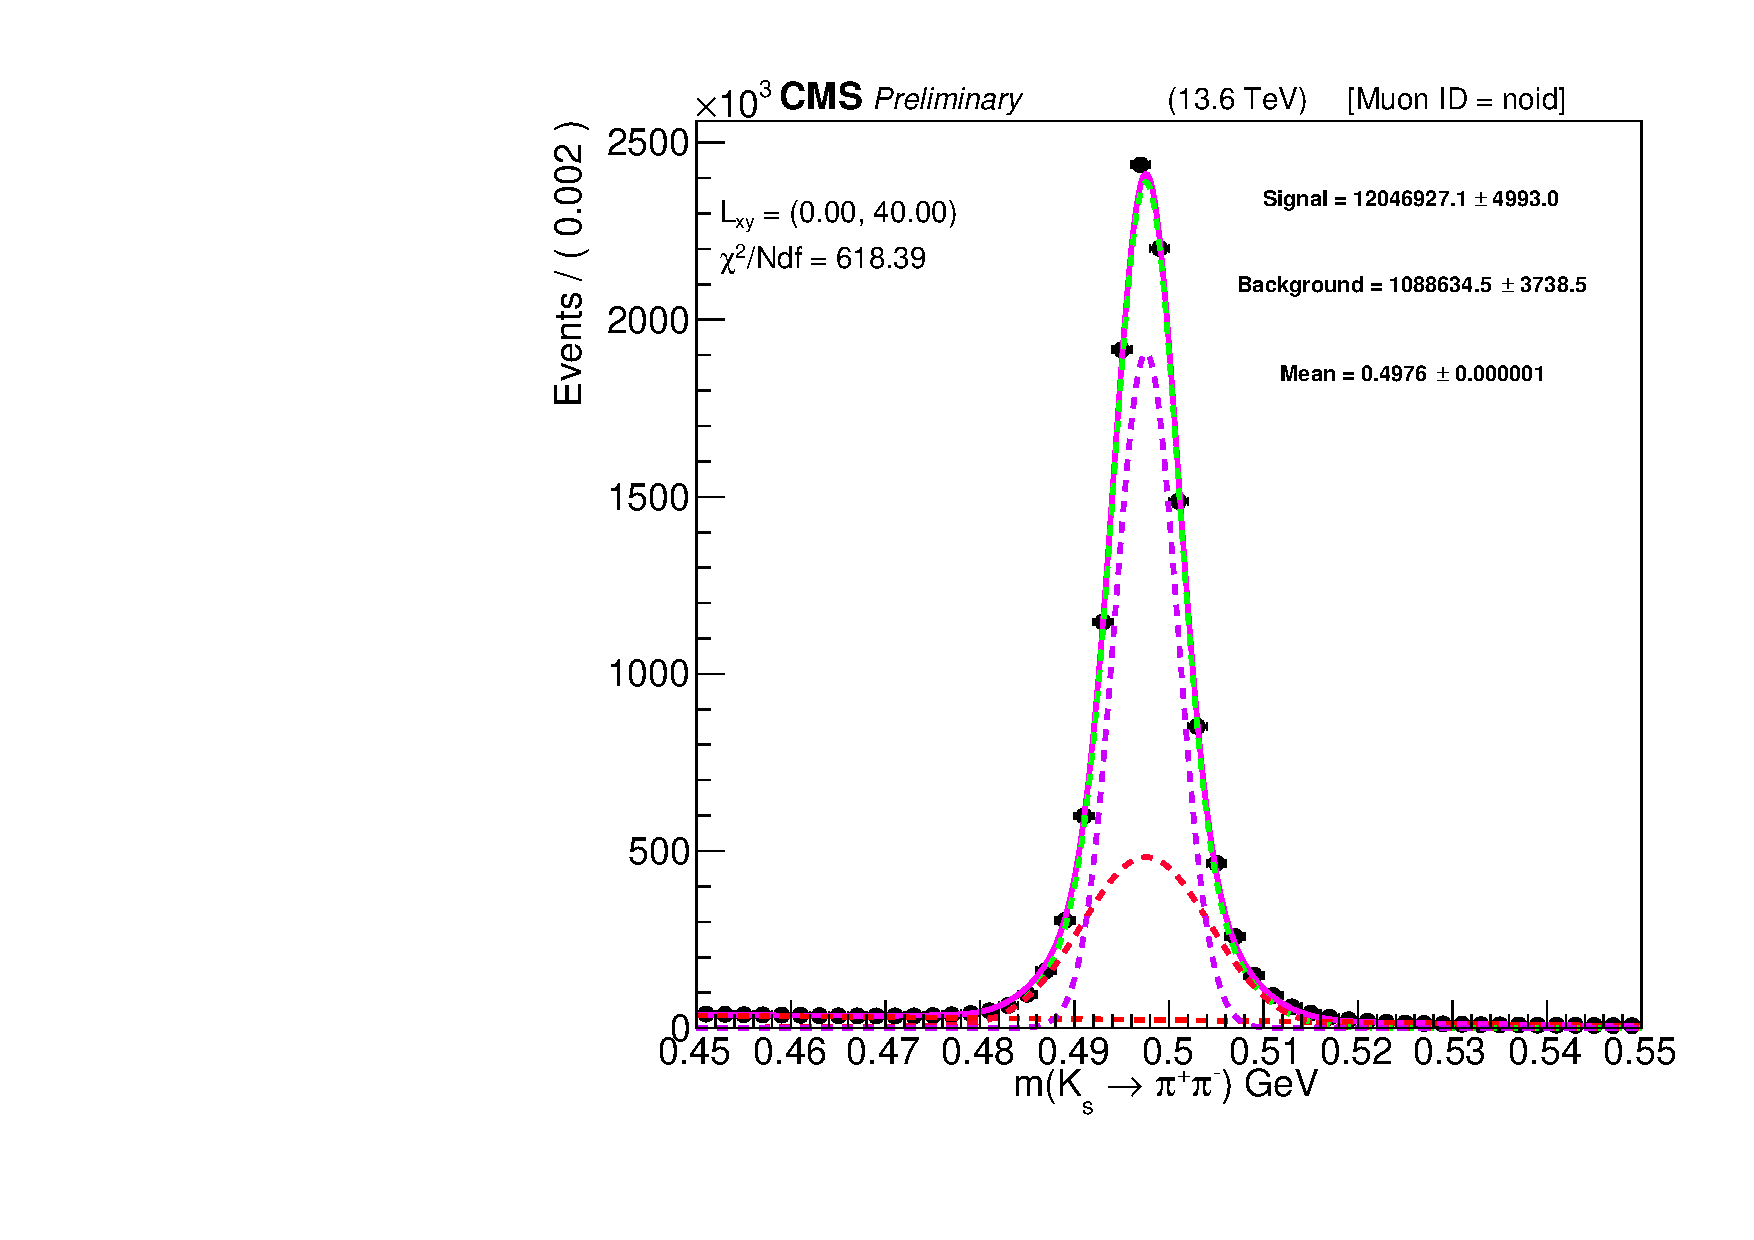
\includegraphics[width=0.45\textwidth]{figures/chapter4/fakerate/Combined_data_combined_522_2022_ks_trigger_lxy_hv0_Mass_allbin_bla.pdf}
    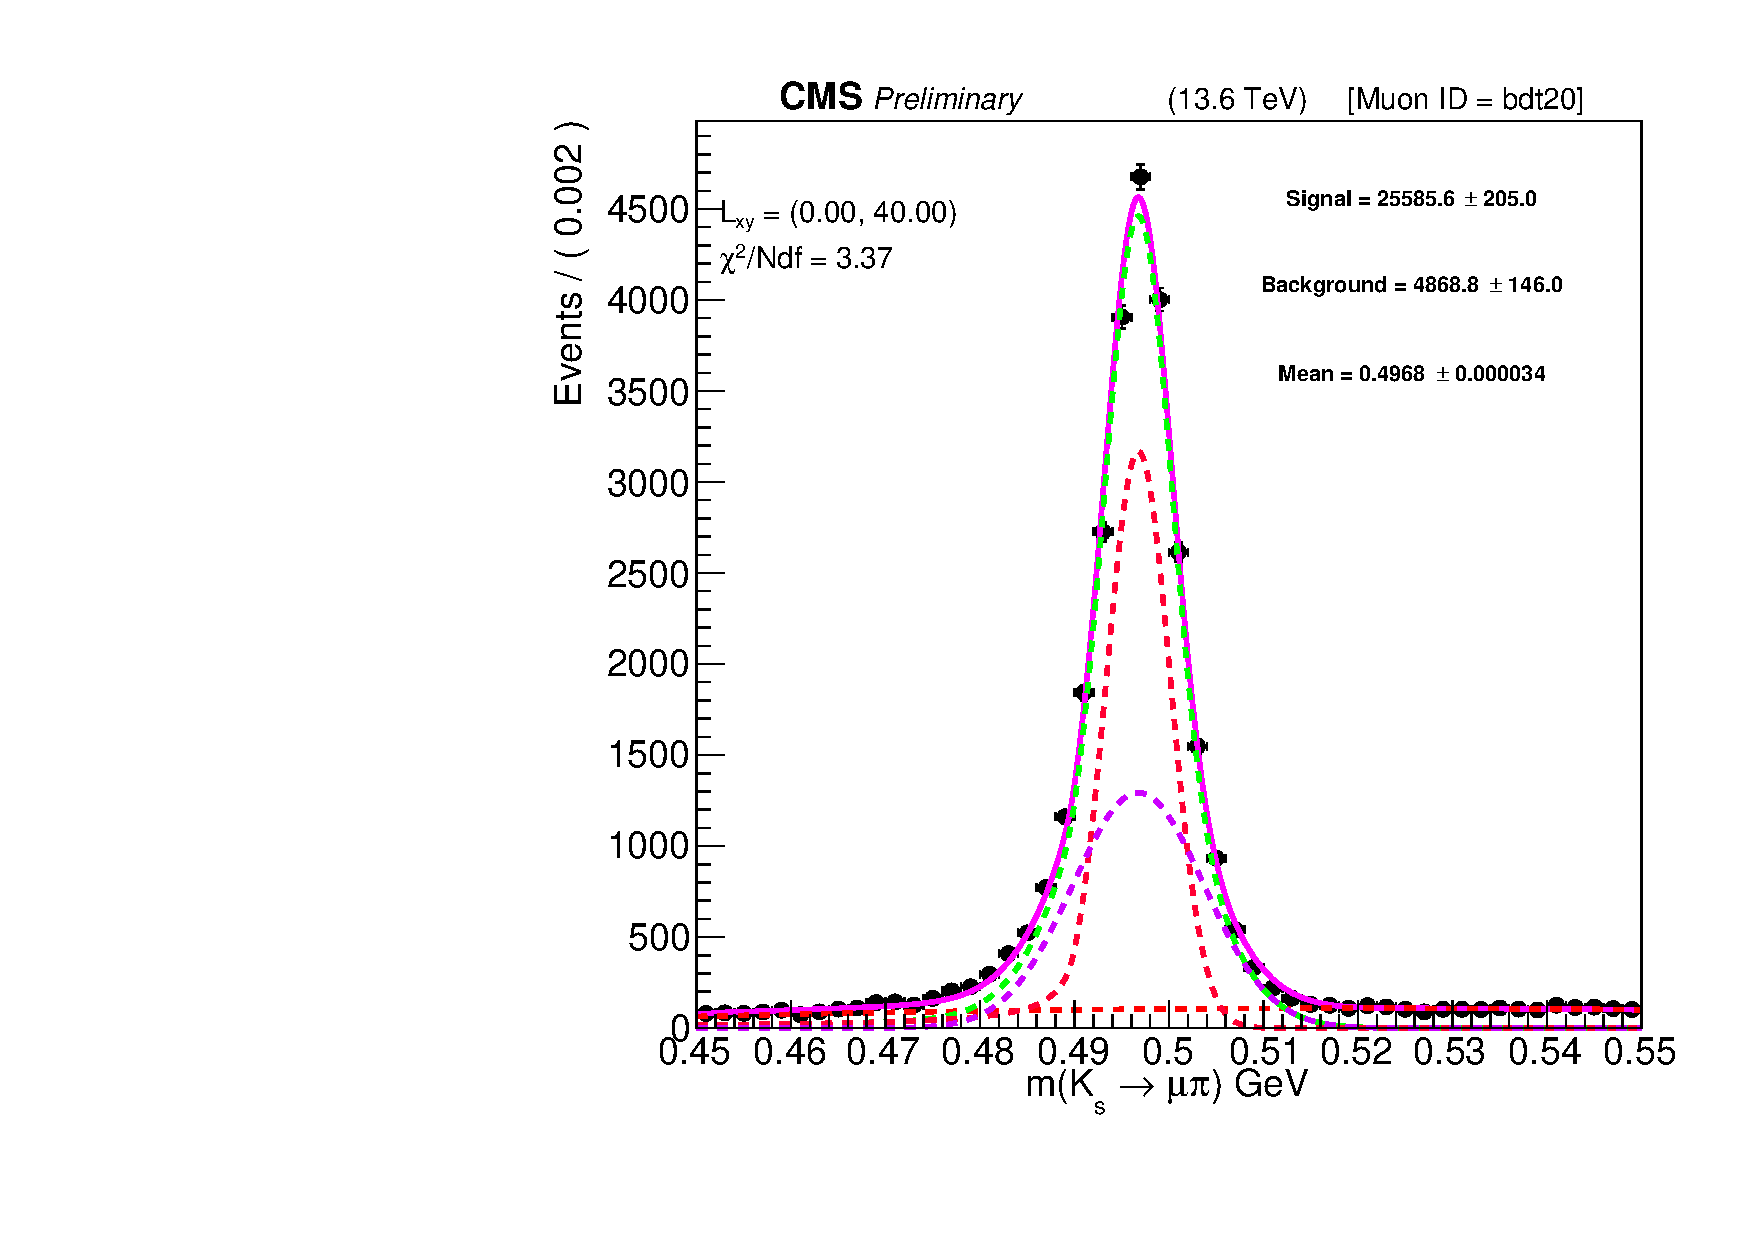
\includegraphics[width=0.45\textwidth]{figures/chapter4/fakerate/Combined_data_combined_522_2022_ks_trigger_lxy_hv0_Mass_muid_20_allbin_bla.pdf}\\
  \end{center}
  \caption{Invariant mass projection from $K_S^0 \to \pi^+ \pi^-$ decays in the $\mu$
    $p_{T}$ range 4-40.0 GeV using 2022 data before (left) and after(right) soft muon MVA ID cut.
    The green dashed line is for the signal distribution, the red
    dotted line is for combinatorial background, and the result of the
    fit projection is the solid pink line. The data are shown with
    solid black circles.}
  \label{fig:fit_example_pion}
\end{figure}

The fake rate is estimated in bins of muon $p_{T}$. For each $K_S^0 \to \pi^+ \pi^-$ candidate we check $p_{T}$ and acceptance for both pions and add the $K_S^0$ candidate to the appropriate $p_{T}$ bin (\ref{fig:fakerates}).

\begin{figure}[!h]
  \begin{center}
    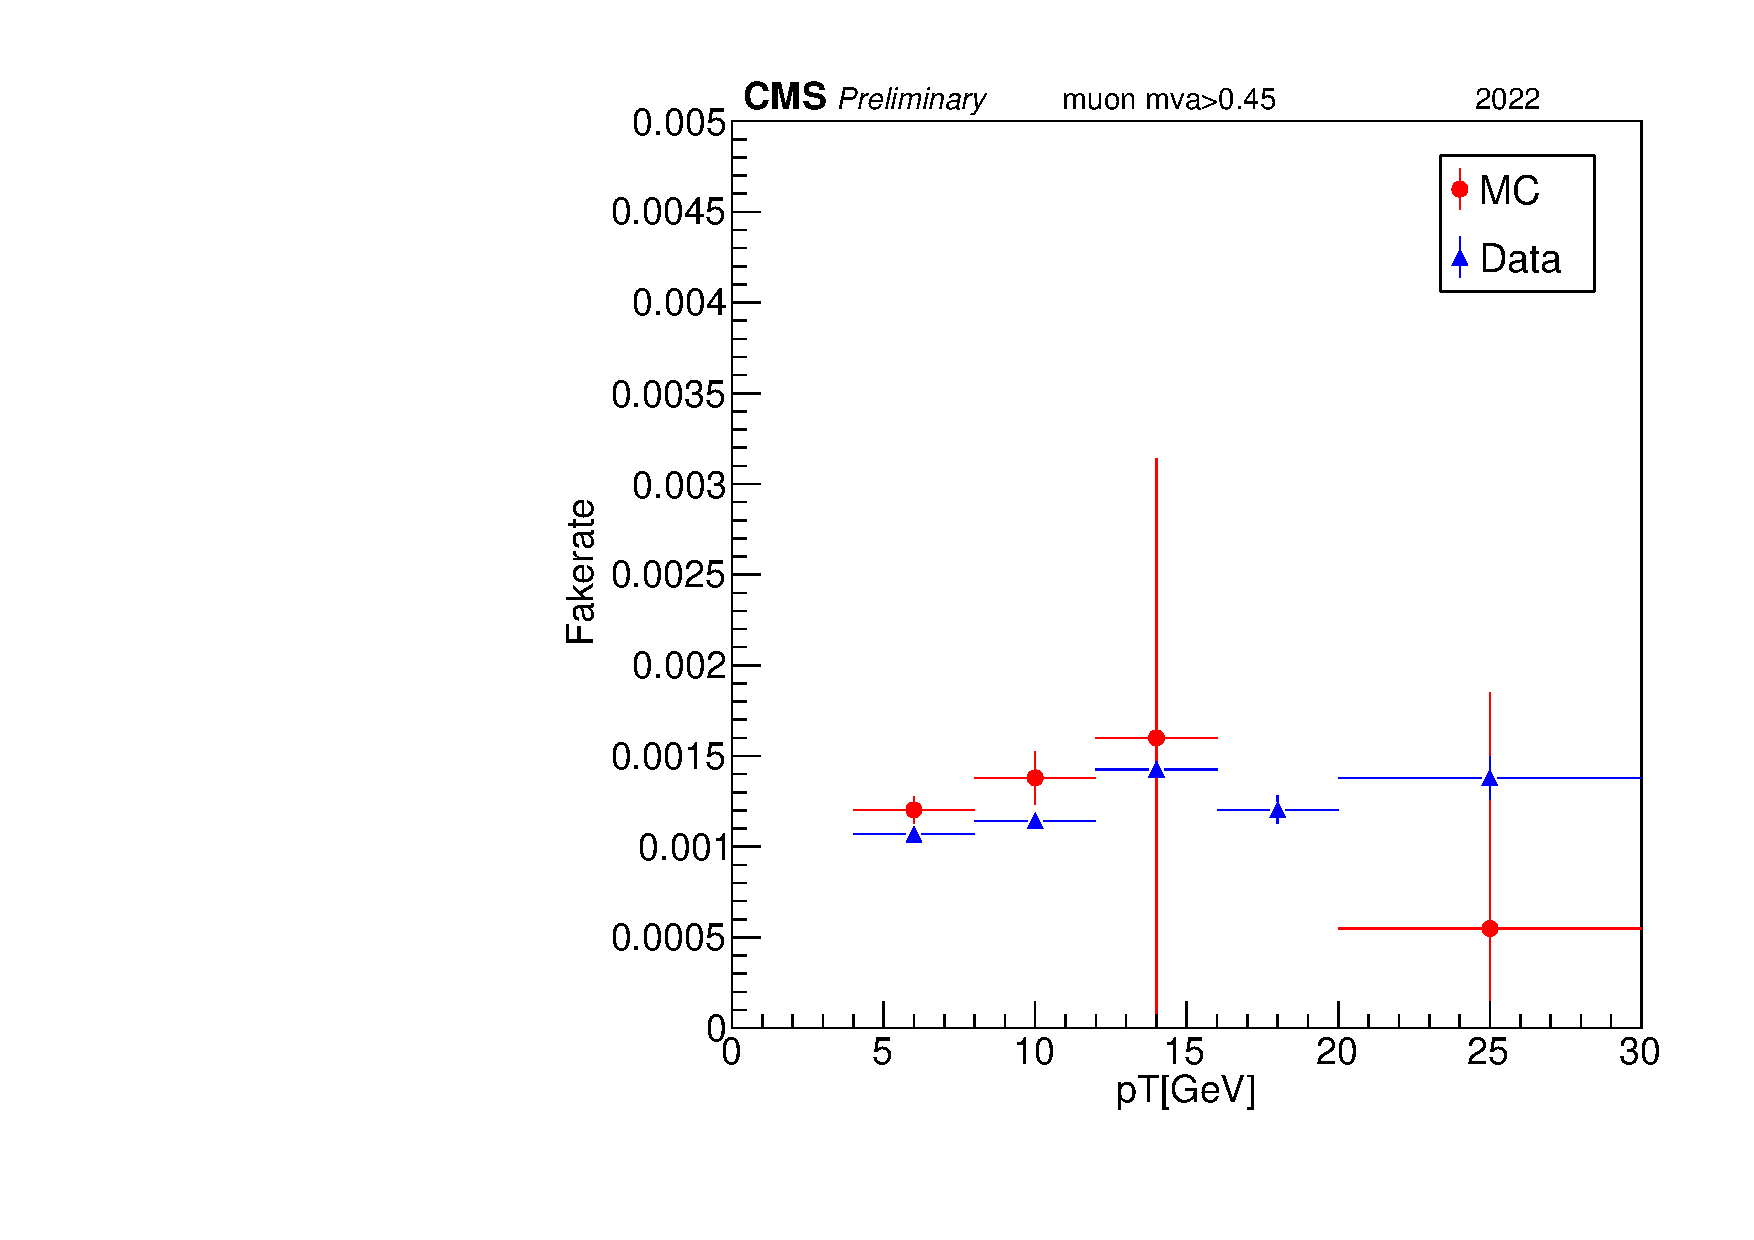
\includegraphics[width=0.45\textwidth]{figures/chapter4/fakerate/Run2022_pion-fakes.pdf}
    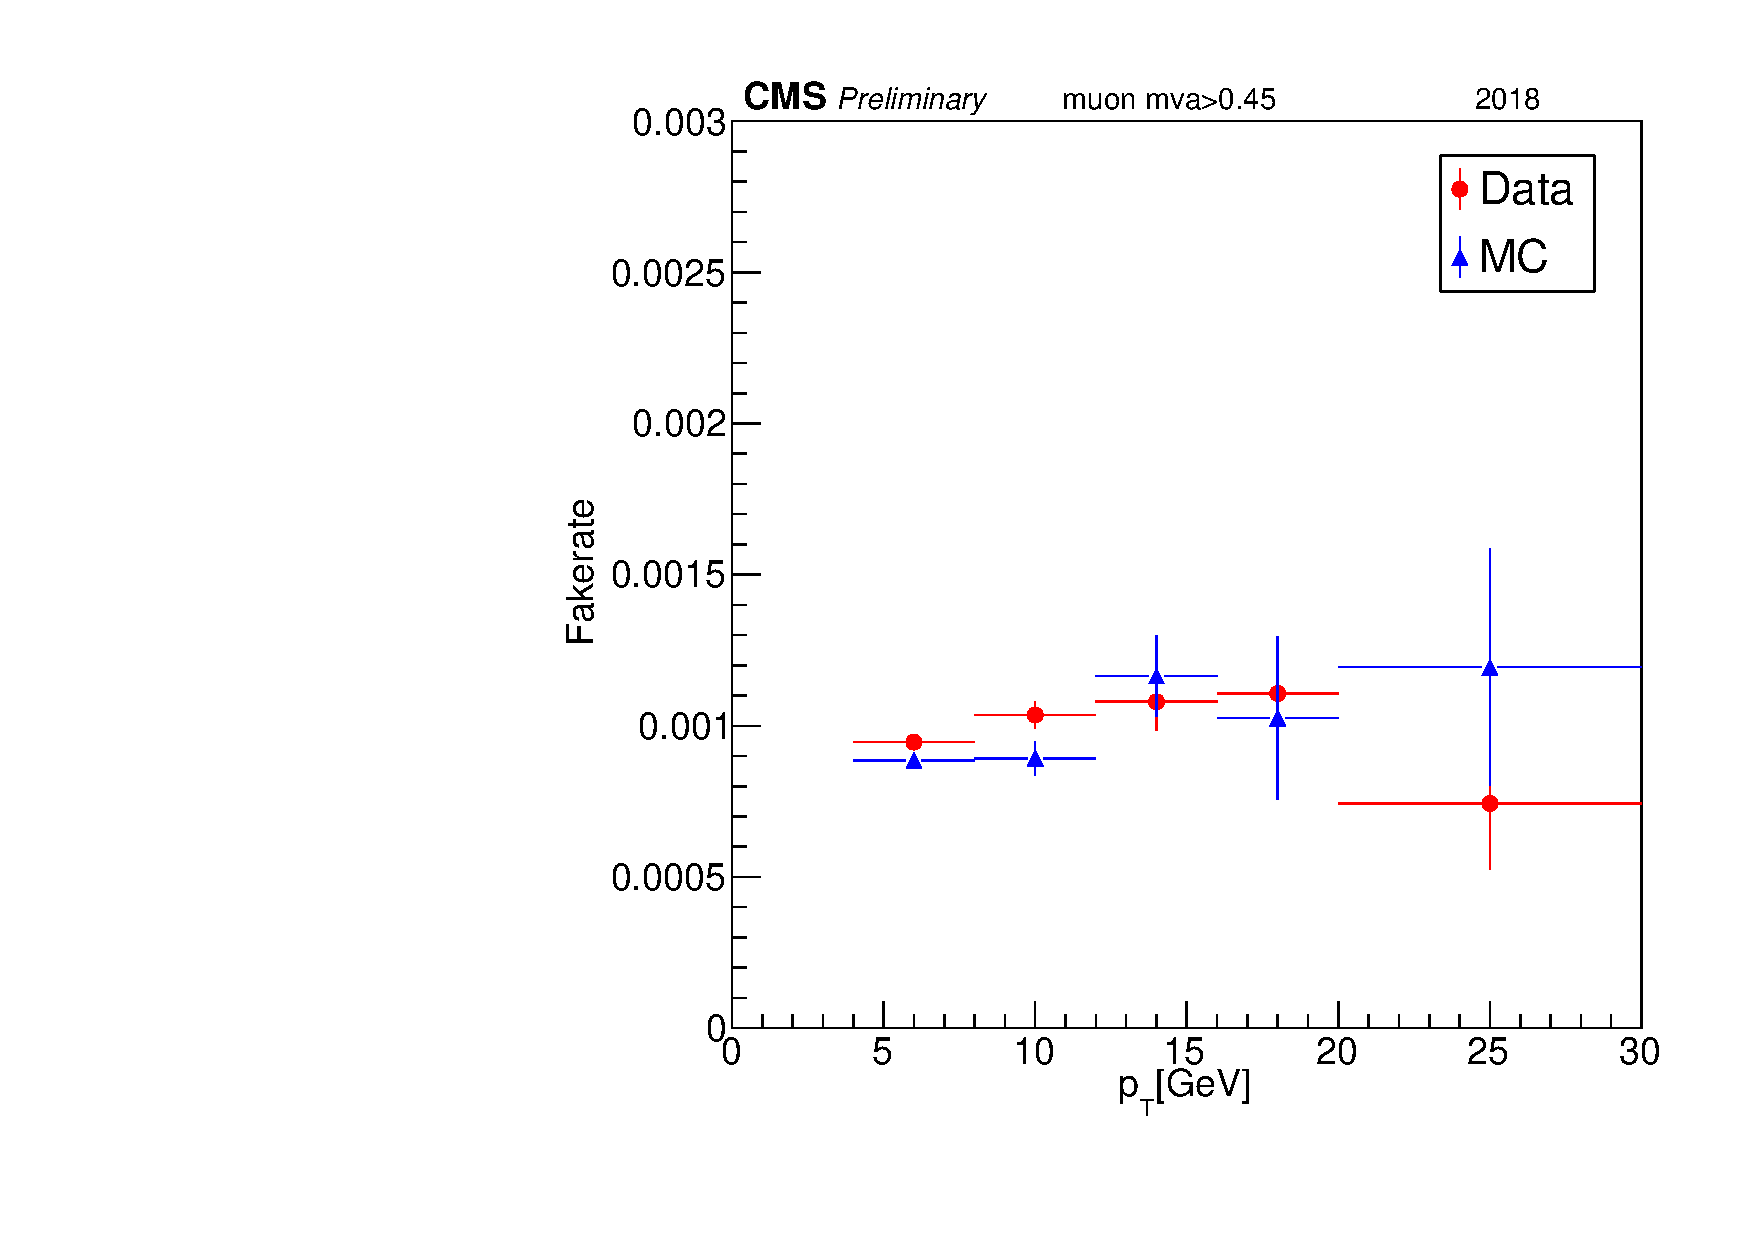
\includegraphics[width=0.45\textwidth]{figures/chapter4/fakerate/Run2023_pion-fakes.pdf}
    \caption{Pion muon fake rates for Run2022 (top) and
      Run2023 (bottom) as a function muon $p_{T}$.}
    \label{fig:fakerates}
  \end{center}
\end{figure}


The fake rate estimated from $K_S^0$ decays also has a dependence on the $K_S^0$ flight length (Figure \ref{fig:pion_fake_rate_fs_flight_length}). There are two different trends. The first is the fake rate increase with the flight length, which is most pronounced for the Loose muon selection. The second one shows a dramatic decrease in the fake rate for muon candidates passing the Soft Muon MVA selection when they originate outside of the pixel detector (fligt length greater than 8 cm).

\begin{figure}[!h]
  \begin{center}
    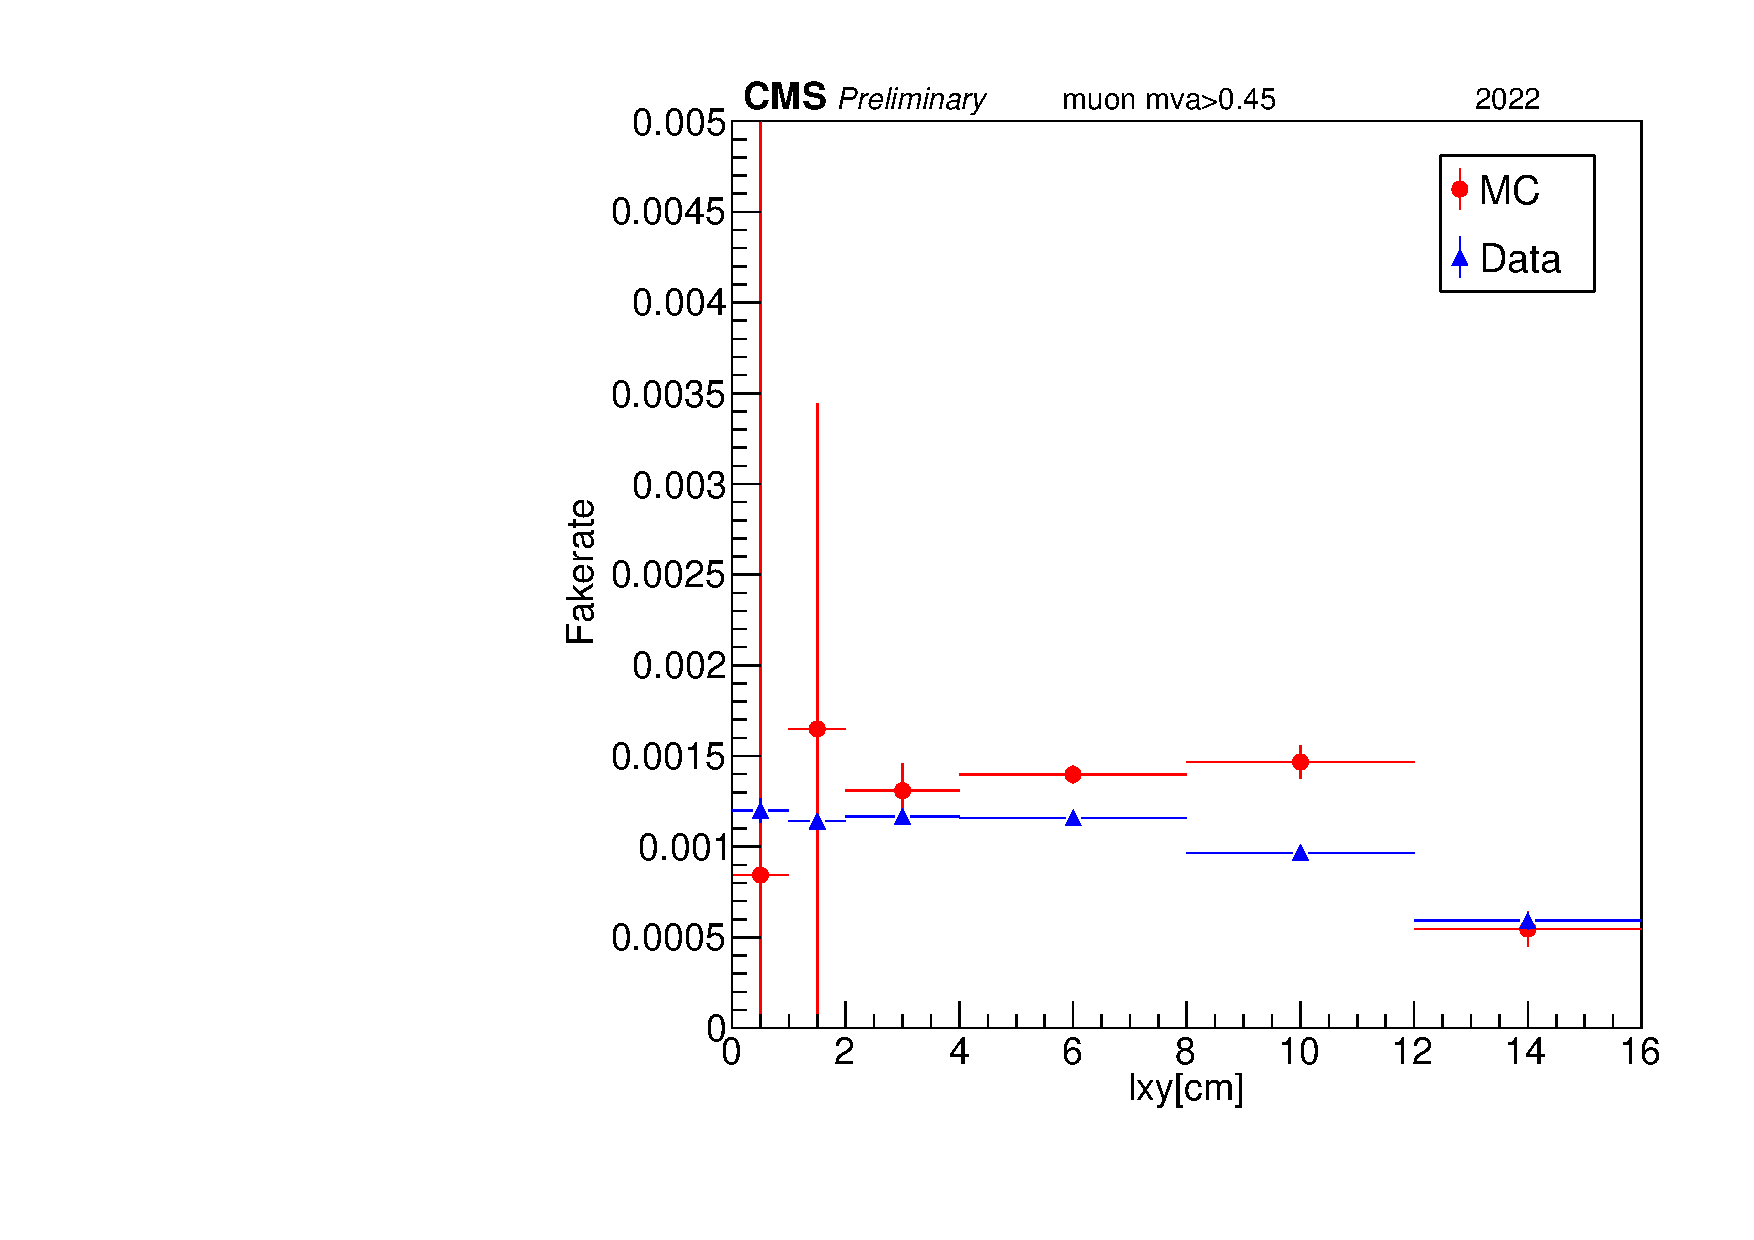
\includegraphics[width=0.45\textwidth]{figures/chapter4/fakerate/playV0-ks_kin_lxy_muidbdt45_MC_v_Data_overlay.pdf}
  \end{center}
  \caption{Fake rate dependence on flight length (lxy) measured in cm for data and MC}
  \label{fig:pion_fake_rate_fs_flight_length}
\end{figure}

Both effects are related to the number of pixel and silicon stip hits for the inner track, which is known to be smaller for fake muons. In the case of the Loose selection this information is not used directly for the muon identification, while for the Soft Muon MVA it is one of the most powerful discriminators. The fact that the fake rate has a non-trivial dependence on the flight length means that we have to match the flight length of the fakes used in the physics analysis to the one available in the control sample. Otherwise, this dependence can lead to a biased measurement of the fake rate since most $K_S^0$ have much larger flight length than the D mesons used in this analysis. Therefore, we restrict the transverse decay length to 8 cm to match the $D$ mesons studied in the analysis. In this region, the fakerate seems to relatively flat and there is enough data to make precise estimates of the fake rate in this region. 

Systematic error for the fake rates measurements in MC samples are derived from taking the weighted differences between the various MC samples used, namely W+Jets, Drell-Yan, and TT bar. Furthermore, systematic error for the fake rate measurements in data is mainly derived  from the differences between EGamma and Parking Electron datasets. Agreement between these datasets can be seen in the plots (\ref{fig:pion_fake_rate_systematics}). To account for the variation in terms of the $l_{xy}$ value, an additional $2\%$ of systematic uncertainty is assigned, motivated by the scale factor variation in terms of $p_T$ and $l_{xy}$ between data collected in 2022 and data collected in 2023. 

The final fake rate results are summarized in table \ref{tab:muon_fake_rate}.

\begin{figure}[!h]
  \begin{center}
    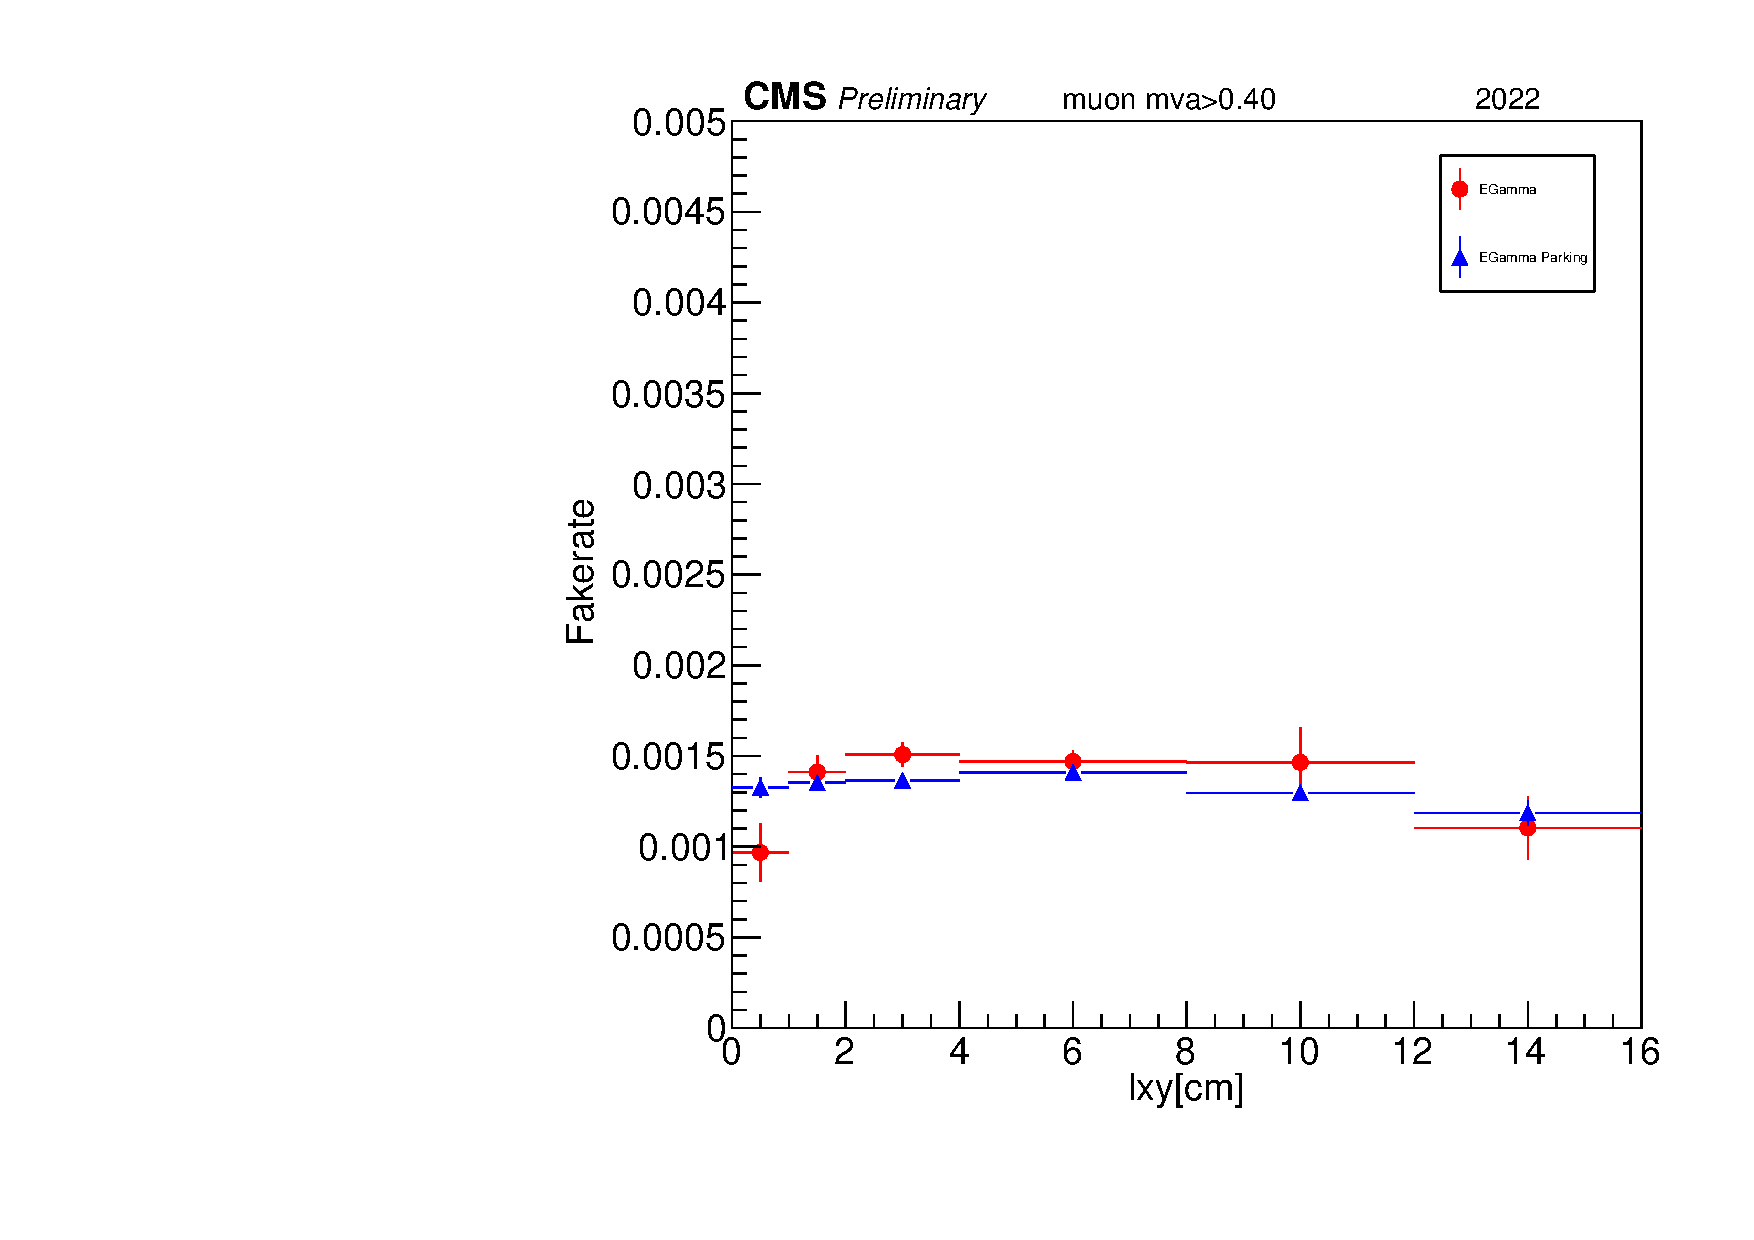
\includegraphics[width=0.45\textwidth]{figures/chapter4/fakerate/playV0-ks_kin_lxy_muidbdt40_EGamma_v_Parking_overlay.pdf}
    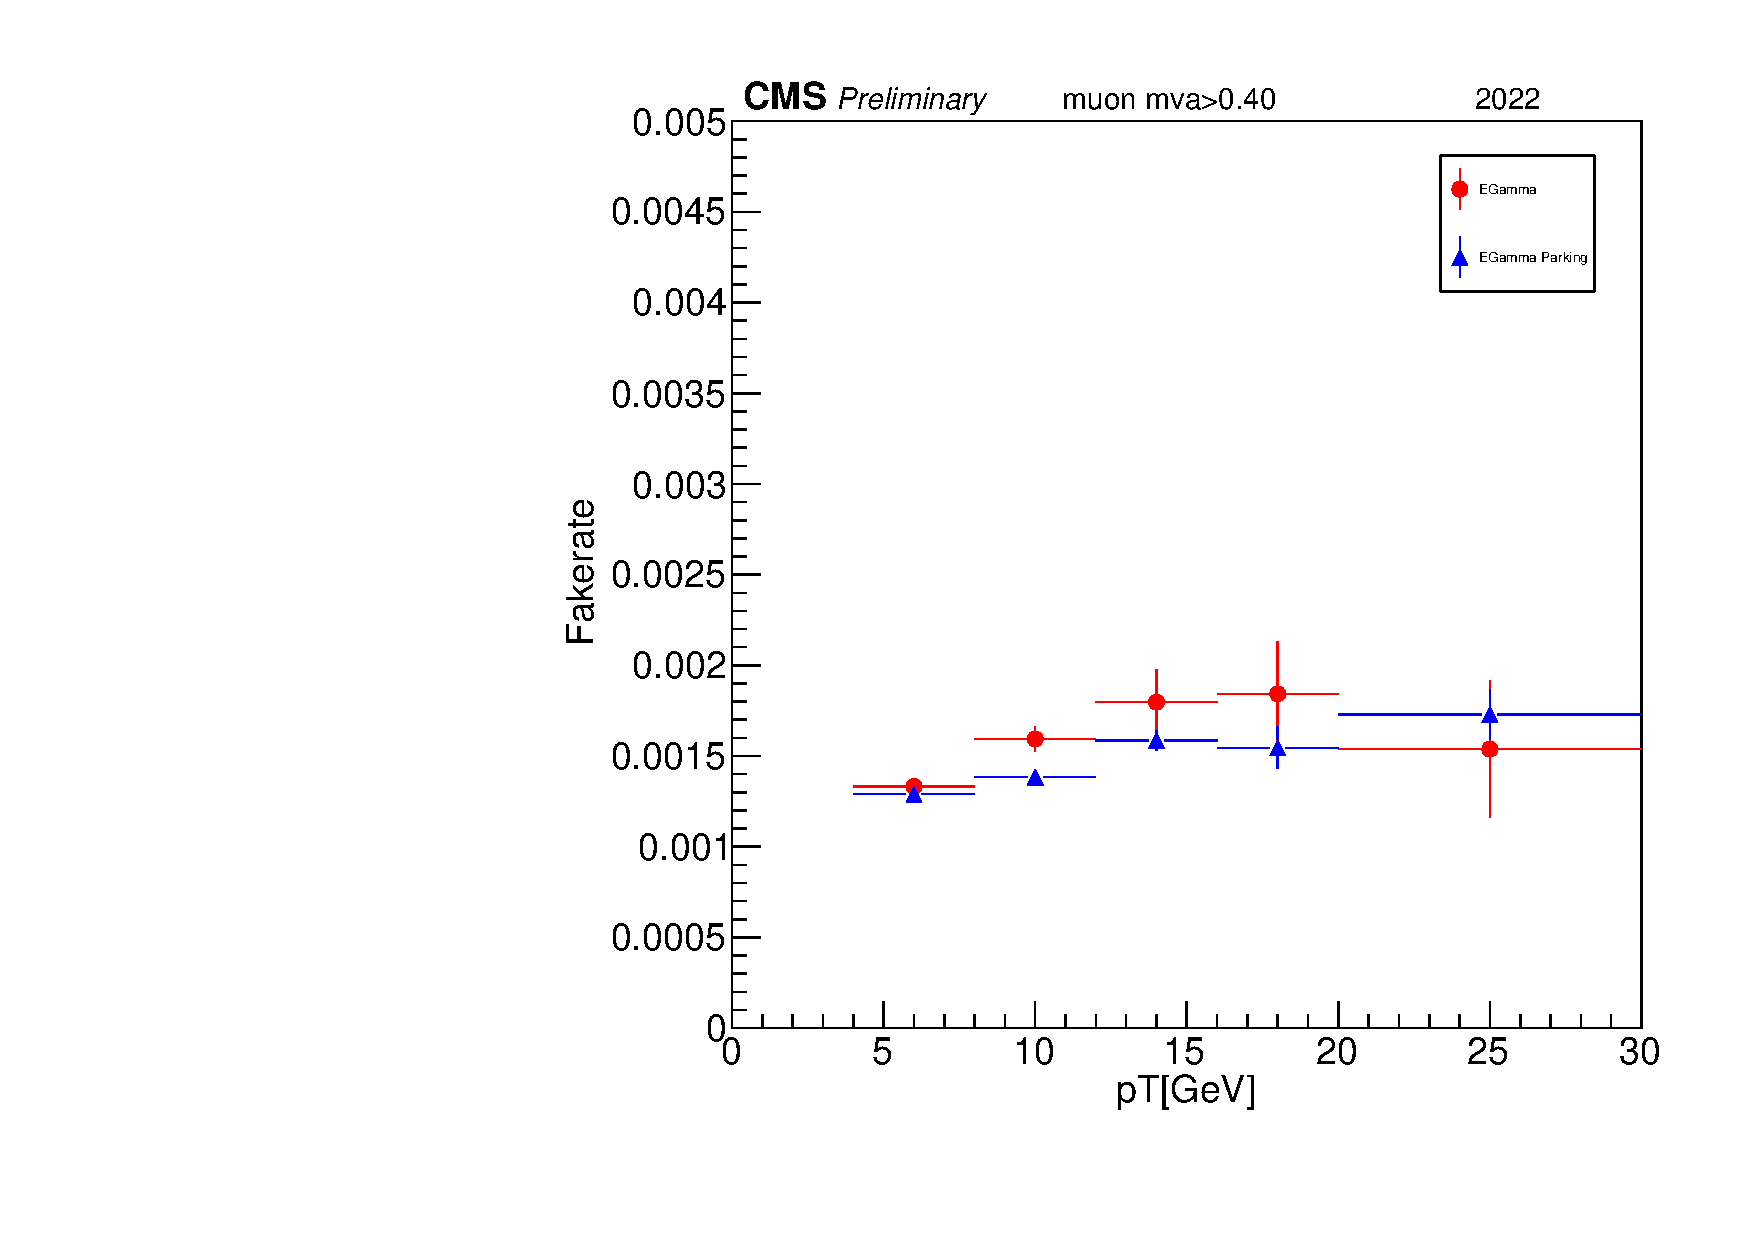
\includegraphics[width=0.45\textwidth]{figures/chapter4/fakerate/playV0-ks_kin_pT_muidbdt40_EGamma_v_Parking_overlay.pdf} \\
    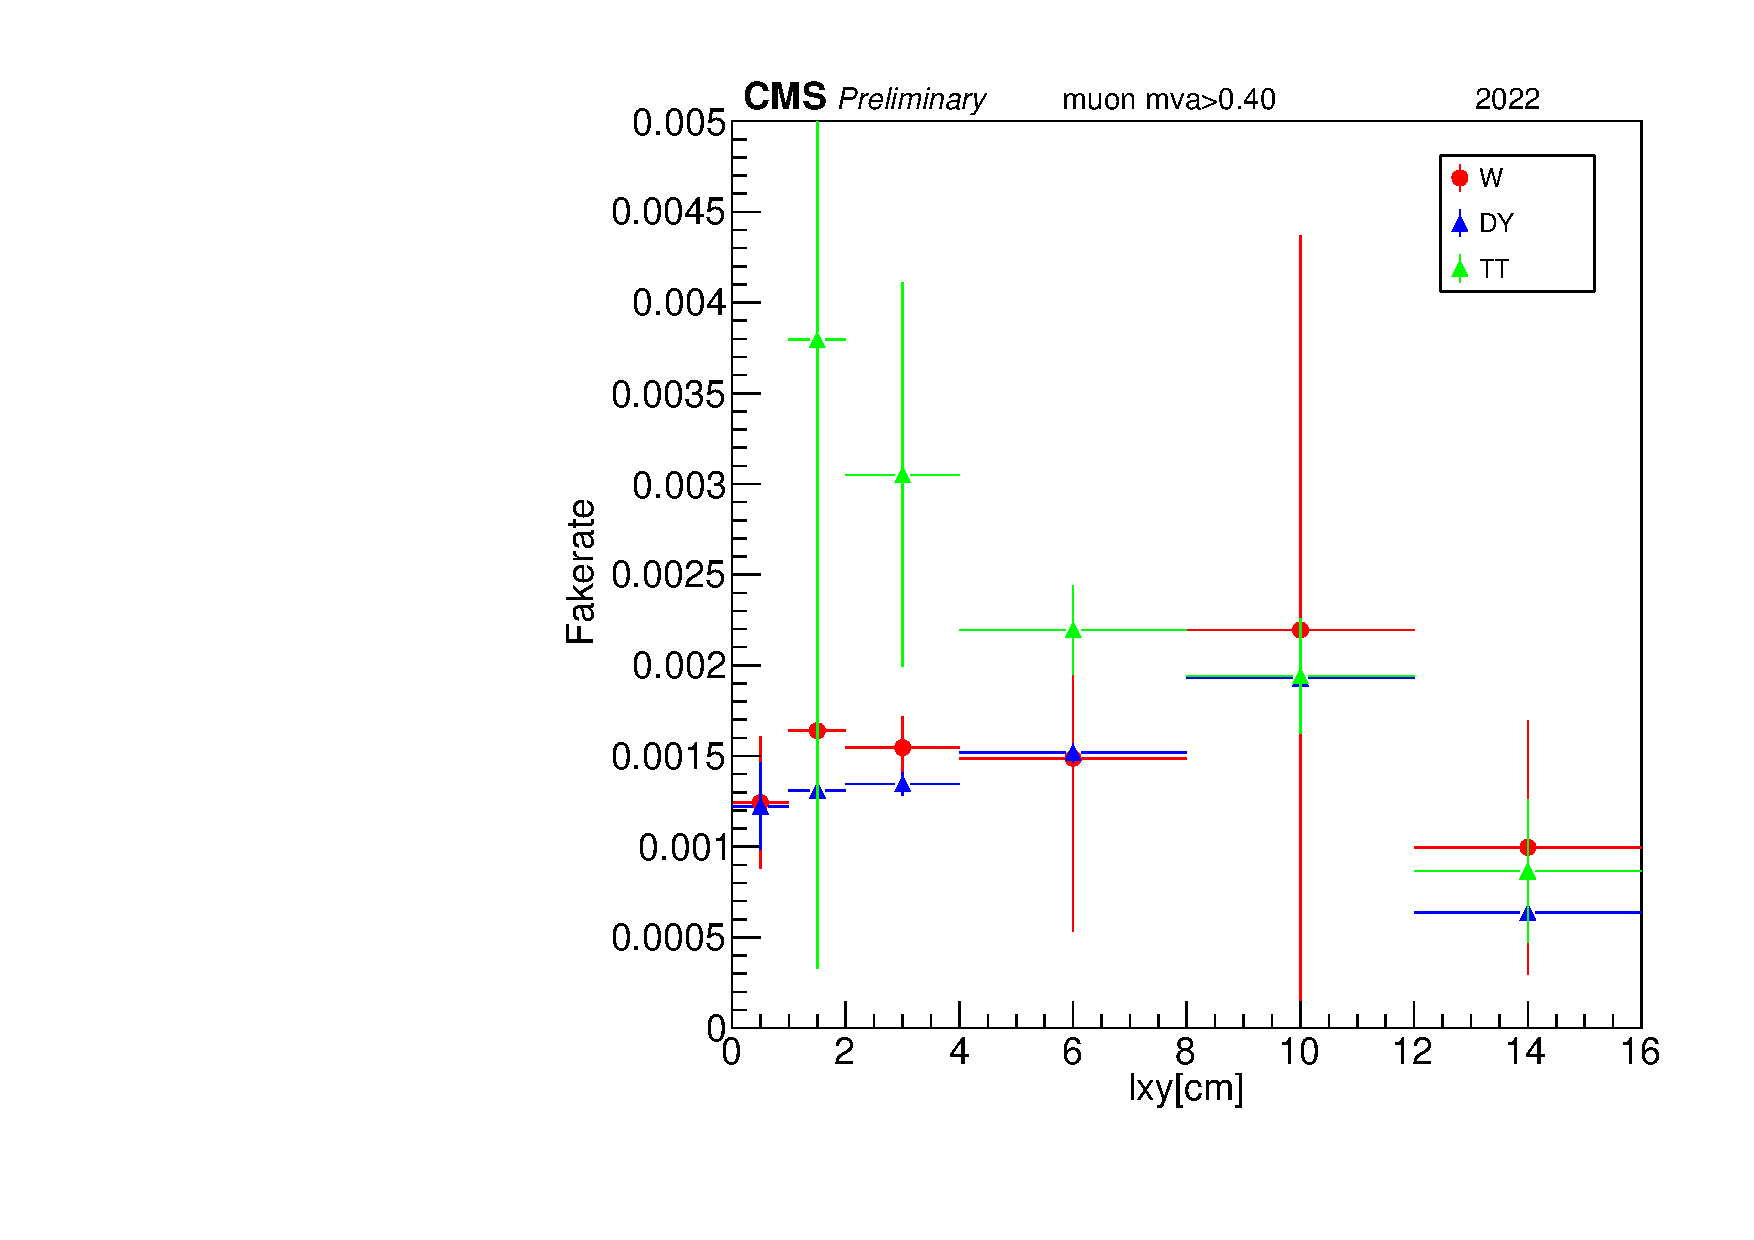
\includegraphics[width=0.45\textwidth]{figures/chapter4/fakerate/playV0-ks_kin_lxy_muidbdt40_W_v_DY_v_TT_overlay.pdf}
    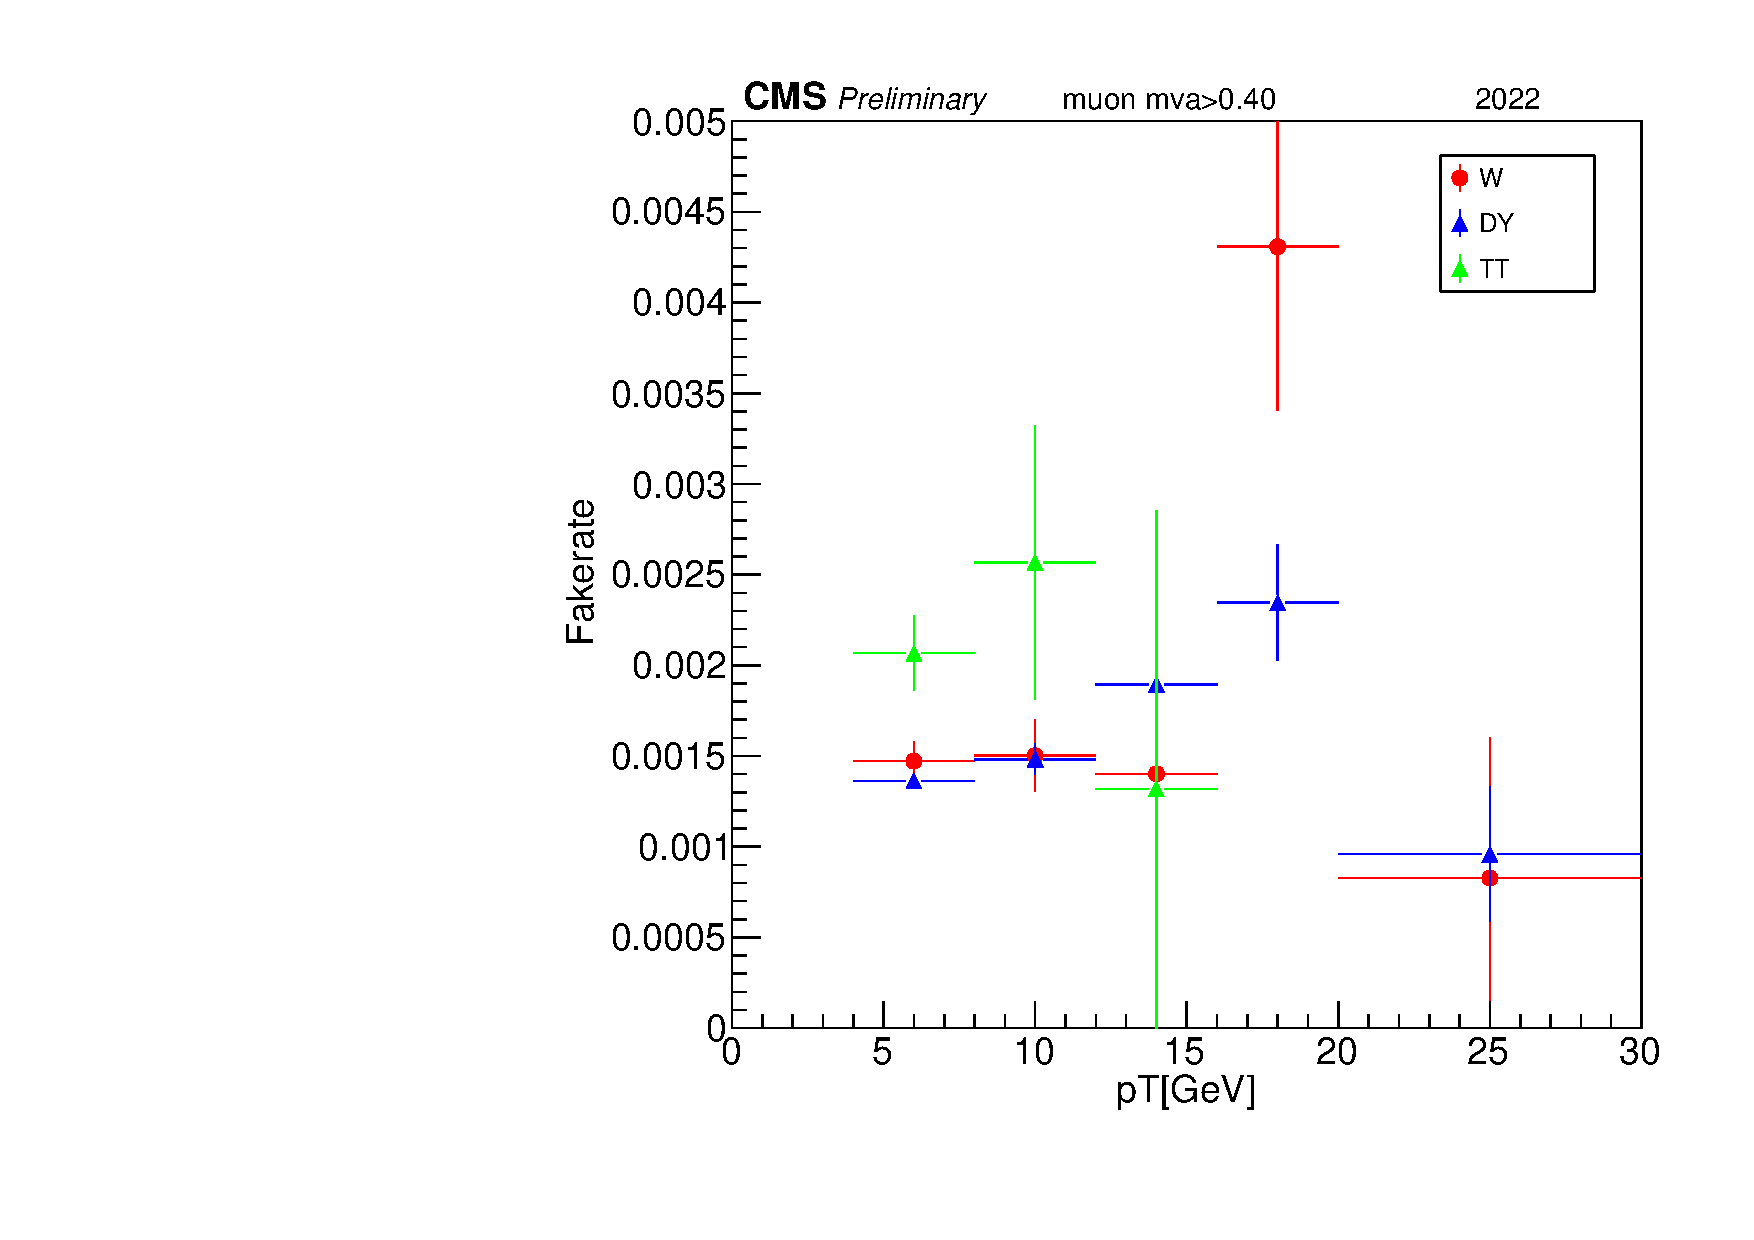
\includegraphics[width=0.45\textwidth]{figures/chapter4/fakerate/playV0-ks_kin_pT_muidbdt40_W_v_DY_v_TT_overlay.pdf}
  \end{center}
  \caption{Difference in fakerate between Egamma and Parking Electron data (top) and W plus jets, Drell-Yan, and TT bar MC samples (bottom) binned by flight length in cm (left) and pT in Gev (right)}
  \label{fig:pion_fake_rate_systematics}
\end{figure}

\begin{table}[htbp]
    \centering
    \begin{tabular}{|c|c|c|c|c|c|c|}
    \hline
     & \textbf{4--8 GeV} & \textbf{8--12 GeV} & \textbf{12--16 GeV} & \textbf{16--20 GeV} & \textbf{20--30 GeV} & \textbf{Total} \\
    \hline
    Run2022 & $1.05 \pm 0.03$ & $0.98 \pm 0.04$ & $1.11 \pm 0.09$ & $1.00 \pm 0.15$ & $1.38 \pm 0.46$ & $1.06 \pm 0.07$ \\
    Run2023 & $1.09 \pm 0.04$ & $0.95 \pm 0.04$ & $1.04 \pm 0.13$ & $1.08 \pm 0.17$ & $1.27 \pm 0.34$ & $1.03 \pm 0.07$ \\
    \hline
    \end{tabular}
    \caption{Muon fake rate ratios for Data over MC simulation for 2022 and 2023 in the bins of meson $p_\mathrm{T}$.}
    \label{tab:muon_fake_rate}
\end{table}


\section{Efficiency Corrections}
\label{sec:efficiency_corrections}

%TODO probably need to rewrite efficiency section in light of this section...

Virtually all selection efficiencies used for this analysis are measured in MC. Normally, this would be troublesome for the results of the analysis due to MC mismodeling effects that cause the efficiency of MC to be different from the efficiency of the data. In terms of a formula, we get that 
\begin{equation}
    \epsilon_{\text{data}} = \epsilon_{\text{MC}} \times \epsilon_{\text{corr}}
\end{equation}
with mismodeling occurring when $\epsilon_{corr} \neq 1$. 

However, the normalization channel approach used in this analysis means that in all calculations needed for the final result, we only care about a \textit{ratio} of efficiencies. One notices that if the $\epsilon_{\text{corr}}$ is the same for both the normalization and signal channels, it cancels when considering a ratio between normalization and signal channel efficiencies. In fact, we notice that except for trigger selection and $\text{MVA}_D$ selection, the selections are kept exactly the same between signal and normalization channels. Since the $\text{MVA}_D$ and trigger selections are independent of the other selections, we can let the other selection efficiency corrections cancel and only consider corrections to $\text{MVA}_D$ selection and trigger selection. The calculation of the $\text{MVA}_D$ correction, denoted $\text{MVA}_{D,corr}$ has already been discussed extensively in section \ref{subsec:mva}. Therefore, all that is left to consider is the trigger efficiency correction for both the $\texttt{HLT\_ZeroBias}$ trigger and the $\texttt{HLT\_DoubleMu4\_3\_LowMass}$ trigger. 

\subsection{Trigger Efficiency Correction}
\label{subsec:trigger_efficency_correction}

Trigger efficiency quantifies how often the trigger fires on events that the trigger is built to capture. For example, the efficiency of the $\texttt{HLT\_DoubleMu4\_3\_LowMass}$ trigger can be calculated as the percentage of low-mass dimuon events that are successfully captured by the trigger. As discussed in section \ref{sec:efficiency_corrections}, the trigger efficiency correction is the ratio of the trigger efficiency in data over the trigger efficiency in MC, used to account for MC mismodeling effects. For our analysis, the trigger efficiency correction of both the $\texttt{HLT\_ZeroBias}$ trigger and the $\texttt{HLT\_DoubleMu4\_3\_LowMass}$ trigger must be found. However, by definition, the $\texttt{HLT\_ZeroBias}$ trigger selects events with no bias, therefore it has $100\%$ efficiency in both data and MC, causing its trigger efficiency correction to be 1. Therefore, in this analysis we only calculate the trigger efficiency correction of the $\texttt{HLT\_DoubleMu4\_3\_LowMass}$ trigger and label it $T_{\text{cor}}$. As is covered in section \ref{sec:triggers}, the triggers are split up into HLT and L1 triggering systems. Therefore, it is convenient for us to calculate their efficiency corrections separately and then combine them to get $T_{\text{cor}} = T_{\text{cor, L1}} \times T_{\text{cor, HLT}}$.

Calculating trigger efficiency in MC samples is done by simply calculating how many of the generated events that fit the trigger criterion actually fired the trigger. In data, we don't know how many events there actually were that fit a certain criterion, making this straight-forward calculation impossible. Instead, in data we calculate the trigger efficiency of one trigger with respect to another which we know has virtually $100\%$ efficiency. Specifically, we calculate what percentage of the time the trigger of interest fired for all events where the reference trigger has also fired. For consistency, then, the MC trigger efficiency is calculated using this same method, instead of the straight forward method initially described. Note that when calculating trigger efficiencies, one must carefully take into account trigger prescales, making sure to equate the scaling of both the trigger of interest and reference trigger. Additionally, since the triggers were changed slightly between 2022 and 2023, we calculate the trigger efficiency corrections in each year separately and then combine to get a total efficiency correction.

We begin with calculating the L1 trigger efficiency correction. The $\texttt{HLT\_DoubleMu4\_3\_LowMass}$ trigger has two L1 triggers it uses for selecting muons, named $\texttt{HLT\_Mu4\_L1DoubleMu}$ and $\texttt{HLT\_Mu0\_L1DoubleMu}$. For the L1 trigger efficiency correction calculation, we pick using $\texttt{HLT\_Mu0\_L1DoubleMu}$ and use the other trigger to find the HLT trigger efficiency correction. For the reference trigger, we use $\texttt{HLT\_Mu3\_PFJet40}$ and $\texttt{HLT\_Mu8}$, both intended for L1 trigger efficiency studies. These triggers both have a single muon efficiency of $0.8714$, meaning that the dimuon efficiency can be calculated to be $1- (1-\sqrt{0.8714})^2 = 0.996 \approx 1$. 

Next, we calculate the HLT trigger efficiency correction, or the fraction of events that pass $\texttt{HLT\_DoubleMu4\_3\_LowMass}$ given that they've passed one of the L1 triggers, $\texttt{HLT\_Mu4\_L1DoubleMu}$. By definition, this means that we can use the $\texttt{HLT\_DoubleMu4\_3\_LowMass}$ trigger with respect to the  $\texttt{HLT\_Mu4\_L1DoubleMu}$ trigger to calculate the HLT trigger efficiency. 

The results of these calculations are summarized in table \ref{tab:trigger_efficiency}. Putting these results together, the correction derived for the L1 trigger is $0.990 \pm 0.005$ and the correction derived for the HLT trigger is $0.953 \pm 0.005$. Put together, this results in a total corrective factor of $T_{\text{cor}} = 0.943 \pm 0.007$. 

\begin{table}[ht]
    \centering
    \begin{tabular}{|>{\footnotesize\raggedright\arraybackslash}p{10cm}|c|c|c|}
    \hline
    \textbf{Measurement} & \multicolumn{2}{c|}{\textbf{Efficiency (\%)}} & \textbf{Ratio} \\
    \cline{2-3}
    & \textbf{Data} & \textbf{MC} & \\
    \hline
    \multicolumn{4}{|c|}{\textbf{2022}} \\
    \hline
    HLT\_DoubleMu4\_3\_LowMass \textbf{wrt} HLT\_Mu4\_L1DoubleMu & $90.08 \pm 0.15$ & $94.91 \pm 0.09$ & $0.949 \pm 0.002$ \\
    HLT\_Mu0\_L1DoubleMu \textbf{wrt} HLT\_Mu3\_PFJet40 & $88.61 \pm 0.60$ & $88.72 \pm 0.43$ & $0.999 \pm 0.008$ \\
    HLT\_Mu0\_L1DoubleMu \textbf{wrt} HLT\_Mu8 & $90.51 \pm 0.25$ & $91.39 \pm 0.18$ & $0.990 \pm 0.003$ \\
    \hline
    \multicolumn{4}{|c|}{\textbf{2023}} \\
    \hline
    HLT\_DoubleMu4\_3\_LowMass \textbf{wrt} HLT\_Mu4\_L1DoubleMu & $90.76 \pm 0.15$ & $94.91 \pm 0.09$ & $0.956 \pm 0.002$ \\
    HLT\_Mu0\_L1DoubleMu \textbf{wrt} HLT\_Mu3\_PFJet40 & $87.88 \pm 0.67$ & $88.72 \pm 0.43$ & $0.990 \pm 0.009$ \\
    HLT\_Mu0\_L1DoubleMu \textbf{wrt} HLT\_Mu8 & $90.10 \pm 0.20$ & $91.39 \pm 0.18$ & $0.986 \pm 0.003$ \\
    \hline
    \end{tabular}
    \caption{Trigger efficiency measurements in Data and MC for 2022 and 2023.}
    \label{tab:trigger_efficiency}
\end{table}

\section{Results}

\subsection{The $CL_s$ Method}

The final result of this thesis is presented as a $CL_s$ limit. Therefore, before discussing the results of the thesis I will describe briefly what the $CL_s$ limit is, why it is used, and how to calculate it. 

Modern statistics utilizes two main frameworks for interpreting search results. The first of these frameworks is a Bayesian framework, developed by calculating posteriors using likelihoods generated from data and inferred priors. However, defining priors over complex or untested hypothesis proves difficult and becomes very subjective to the method in which researchers assign priors. Therefore, for many applications, such as this one, the Bayesian approach is incomplete. The second of these frameworks is the frequestist approach, which draws conclusions on the compatibility of data with a given theory. However, in nearly all physical applications, researchers aim to generate conclusions on theory given data. Due to the convergence of Bayesian and frequestist conclusions in experiments with large signals and high backgrounds, researchers often allow themselves to draw conclusions on theory with a frequestist approach. However, this method will not hold here due to the incredibly small signal we are searching for.

To figure out what technology to use instead of these methods, we analyze carefully what goes wrong with a standard confidence interval test. The fundamental problem of these tests is that without proper prior weighting of hypothesis, one rejects hypothesis which the experiment had no sensitivity to. More specifically, confidence intervals can tell you about the validity of a hypothosis without considering how likely it is that the hypothesis can be proven wrong. This is what the $CL_s$ method fixes; it takes the p-value of the signal+background model used in confidence intervals and divides it by the one minus p-value of the background. Therefore, if the model for the signal+background hypothesis is close to the model for the background-only hypothesis, the $CL_s$ method imposes a penalty due to the lack of sensitivity in the experiment. 

The fundamental building block for the $CL_s$ method is the likelihood ratio test statistic, 
\begin{equation}
    Q = -2 \ln \left(\frac{\mathcal{L}(s+b)}{\mathcal{L}(b)}\right)
\end{equation}
where $\mathcal{L}(s+b)$ is the likelihood calculated by the UML fit described in section \ref{sec:UML} and $\mathcal{L}(b)$ is the likelihood calculated using the same fit but excluding the signal model. This means that small $Q$ values correspond to fits that indicate a stronger signal+background fit than background-only fit. 

Now, recall from section \ref{sec:UML} that the likelihood is dependent on the nuisance parameters as well as the parameter of interest. Therefore, we adjust our notation briefly to reflect this, writing $\mathcal{L}_{(b)}(\theta, \vec{\theta}_N)$ and $\mathcal{L}_{(s+b)}(\theta, \vec{\theta}_N)$ to represent the likelihoods. In this experiment, like many others, there are many nuisance parameters that complicate the shape of the likelihood, increase computational complexity, and cause us to track an unmanageable amount of uncertainties. To avoid these issues, we introduce the profile liklihood, $\mathcal{L}_p(\theta) = \max_{\vec{\theta}_N} \mathcal{L}(\theta, \vec{\theta}_N)$. Note that this is not a real likelihood due to the fact that it does not reflect uncertainties in nuisance parameters. However, the test statistic $Q_p$ obtained from the profile likelihood ratio is equivalent to the full likelihood ratio test statistic. For this reason, in virtually every analysis (including this one) the profile likelihood is used. Additionally, due to the lack of impact on the validity of the test statistic, we drop that $\mathcal{L}_p$ and $Q_p$ notation for the remainder of the discussions in this thesis. However, it is important to remember that we are always using profile likelihoods instead of true liklihoods in this analysis. 

Now that we have generated the basic formalism needed to discuss $CL_s$ methods, there are two main applications of $CL_s$ that are used in every experiment. These applications are (i) scanning analysis variables for the best expected limit and (ii) finding the bound of the parameter of interest based on unblinded data. Both these applications are discussed below and later applied to the analysis in section \ref{subsec:sensitivity_scan} and section \ref{subsec:final_result}.

\subsubsection{Limit Calculation Using Real Data}
\label{subsubsec:limit_calculation_theory}

In many $CL_s$ experiments, the goal is to put a limit on a parameter of a physical theory using observed data. This is typically done once the entire analysis has been frozen and only the unblinding is left. Before starting the $CL_s$ method, one picks the confidence level that you would like to have, denoted $CL$. Common $CL$ values are $90\%$ and $95\%$. 

To begin, $n$ toy experiments are generated under a background-only hypothesis and for each of these toys, a $Q$ value is generated, giving a distribution of $n$, $Q_b$ values. In the case of this analysis, this is straight forward since our background model is in the form of a PDF as described in section \ref{sec:UML}. Therefore, one simply samples from the background PDF to generate background-only toy data. 

Once the background-only test statistic distribution is complete, one generates a singular $Q_{\text{obs}}$ value based on the actual, observed data. The area under the curve of the $b$ distribution to the left of $Q_{\text{obs}}$ is then calculated and is the $p_b$ value.

Next, $n$ more toy experiments are generated under a signal+background hypothesis, where the signal strength, $s$, is left floating. These toy experiments are constructed using a similar method to the backgrounds, just with the signal+background model for some signal strength, $s$. We denote this distribution of $n$ points $Q_{s+b}(s)$, highlighting its dependence on $s$, the signal strength. From this, the area under the curve of $s+b$ distribution to the right of $Q_{\text{obs}}$ is the p-value (or $p_{s+b}(s)$ value, again denoting the dependence on $s$). 

Then, the $CL_s(s)$ value is determined by calculating
\begin{equation}
    CL_s(s) = \frac{p_{s+b}(s)}{1-p_b}
\label{eq:cls}
\end{equation}
Lastly, the value of $s$ is found such that $CL_s(s) = 1-CL$\footnote{It may seem computationally difficult to do this naively by scanning over $s$ values and generating $n$ toys for each value of $s$. While optimizations exists in certain cases, employing $CL_s$ methods is in practice computationally challenging}. This value of $s$ is then reported as the upper limit. An example of this can be seen in figure \ref{fig:cls_visualization}.

\begin{figure}[h!]
    \begin{center}
      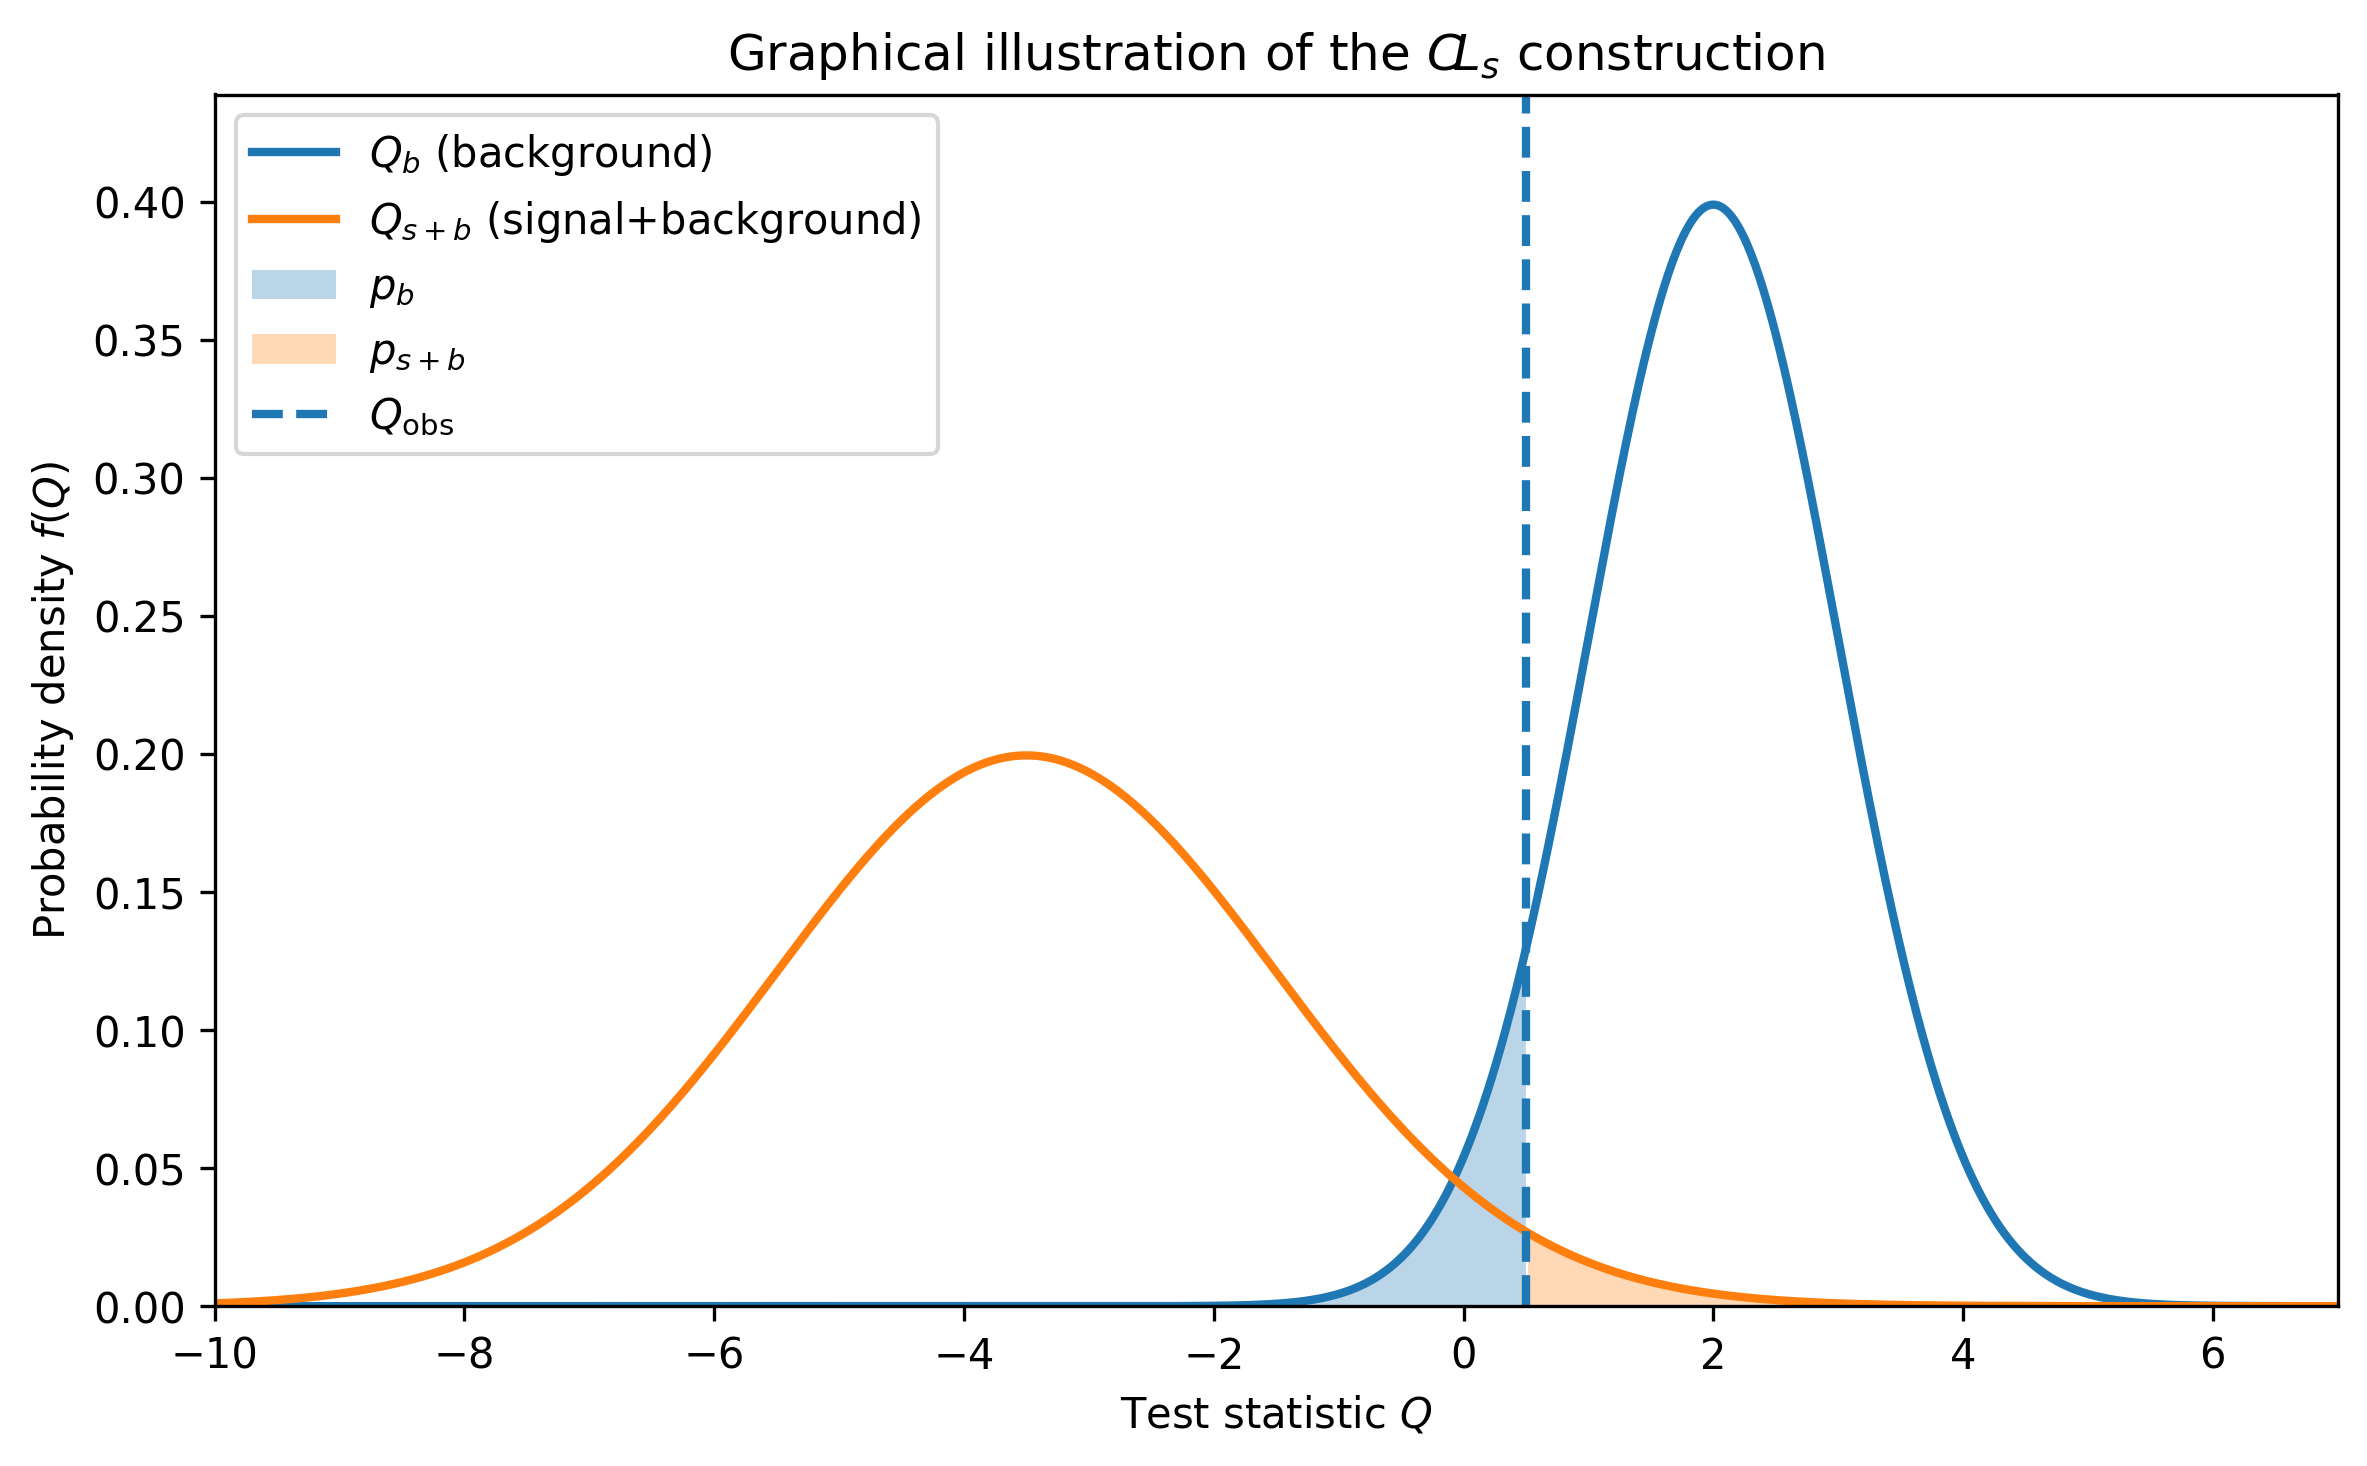
\includegraphics[width=0.8\textwidth]{figures/chapter4/cls_visualization.png}
    \end{center}
    \caption{
      A visualization of the $CL_s$ method, using idealized data and a given signal strength, $s$. 
    }
    \label{fig:cls_visualization}
\end{figure}

\subsubsection{Sensitivity Scanning Using Expected Limits}
\label{subsubsec:sensitivity_scanning_limits}

In many $CL_s$ experiments (including this one), one is interested in tuning a parameter, $\alpha$, in the analysis to get the best experimental outcome. However, this cannot be done directly once the data is unblinded, since this would introduce bias by allowing the observed data to influence the optimization, leading to overfitting. Instead, sensitivity scans are performed using expected limits. To begin, one picks several discrete values of parameter $\alpha$ to test, labeled $\alpha_i$. As before, one additionally picks desired confidence level.

For simplicity, let's assume, for now, that we are not interested in keeping our data blinded during the sensitivity scan and directly have access to the data and therefore $Q_{\text{obs}}$. In this case, the sensitivity scan becomes a straight forward extension of the previous section. Namely, for each $\alpha_i$, distributions of $Q_b$ and $Q_{s+b}(s)$ are generated, the value of $Q_{\text{obs}}$ is obtained given $\alpha_i$, the $CL_s(s)$ value is calculated, and the value of $s$ is found such that $CL_s(s) = 1-CL$. Then, the specific $\alpha_i$ is picked that generates the most sensitive $s$. 

In the case where we don't have access to the real data, we must compute an expected result given simulated data under a given hypothesis. It is common for searches to use background-only hypothesis for this, given that there is typically much evidence for the background-only hypothesis, though more complex choices are possible\footnote{One may be concerned about the freedom of choice for a reference hypothesis. However, recall that this doesn't affect the final limit calculation, just the choice of $\alpha$ that generates the best model sensitivity. If one picks the "wrong" reference hypothesis, one simply finds a worse choice of $\alpha$. In practice, however, most reasonable choices work here to find a good value of $\alpha$.}. There are then two options for computing $Q_{\text{pseudo-observed}}$ to be used instead of $Q_{\text{obs}}$. The first is to again generate toys under the hypothesis of choice to get a distribution of $Q$ values, then take the median of that distribution to get $Q_{\text{pseudo-observed}}$. The second is to generate an Asimov dataset, by simply generating a "perfect" dataset with no statistical fluctuations on the background only model and computing the $Q$ value of this "perfect" dataset. Importantly, this is much cheaper computationally, but requires the conclusion that the median of the toy results is equivalent to the toy result of the median, which requires a Gaussian approximation. In practice, this approximation is typically valid (as is the case in this analysis), so the Asimov dataset approach is used.

There is one more subtly that is worth addressing to complete the $CL_s$ picture. Wilks' theorem states that the profile likelihood ratio, $Q$, distributes asymptotically as a $\chi^2$ distribution with degrees of freedom equal to the difference in the number of floating variables in the signal+background model compared to the background-only model. This implies that, under the asymptotic and null assumption, one doesn't need to generate distributions of $Q_b$ using toys. Instead, one can always use Wilks' theorem to derive the shape of the $Q_b$ distribution from a $\chi^2$ distribution. In practice, this approximation is also well-founded and used in most sensitivity scans, dramatically reducing the number of toys needed. 

\subsection{Sensitivity Scan}
\label{subsec:sensitivity_scan}

Now that the statistical formulation for the final result is complete, we turn back to the calculation of the final result. 

As mentioned in section \ref{subsec:mva}, one of the major benefits of using an $\text{MVA}_D$ cut parameter is that we can tune it to best improve analysis sensitivity. This is done using the technology developed in section \ref{subsubsec:sensitivity_scanning_limits} with two important distinctions to highlight.

Firstly, one might assume that the parameter of interest is the output of the signal channel UML fit, $N_{D^0 \to \mu^+ \mu^-}$. However, this is not quite true as the parameter that we wish to put a limit on is the actual branching fraction $\mathcal{B}(D^0 \to \mu^+ \mu^-)$. The discussion in section \ref{subsec:signal_channel_uml} can be extended to the calculation of $\mathcal{B}(D^0 \to \mu^+ \mu^-)$, resulting in 
\begin{equation}
    \frac{N_{D^0 \to \mu^+  \mu^-}}{N_{D^0 \to \pi^+ \pi^-}} = \frac{\mathcal{B}(D^0 \to \mu^+ \mu^-)}{\mathcal{B}(D^0 \to \pi^+ \pi^-)}\times \frac{\epsilon_{D^*, D^0\to\mu\mu}}{\epsilon_{D^*, D^0\to\pi\pi}} \times S_{ZB} \times \text{MVA}_D \times T_{\text{corr}} 
\end{equation}
where the variables are the same as defined in equation \ref{eq:peaking_background_yield_calculation}. Therefore, to perform the sensitivity scan we don't just calculate $N_{D^0 \to \mu^+ \mu^-}$ under different toy experiments, but rather perform the entire calculation required to derive $\mathcal{B}(D^0 \to \mu^+ \mu^-)$, including the calculation of $\epsilon_X$ and $N_{D^0 \to \pi^+ \pi^-}$ at various $\text{MVA}_D$ working points. Luckily, there are some parameters that don't change, such as $T_{\text{corr}}$ or $S_{ZB}$, so some computation can be saved.

The other important distinction is that under the $\texttt{HLT\_ZeroBias}$ trigger, there are simply too few data points to produce an effective sensitivity scan result. Therefore, to avoid being biased by data fluctuations that prevail when signal events are rare, we include five additional zero bias data. The five triggers of corresponding to the datasets is listed below
\begin{enumerate}
    \item \texttt{HLT\_ZeroBias\_FirstBXAfterTrain}
    \item \texttt{HLT\_ZeroBias\_FirstCollisionAfterAbortGap}
    \item \texttt{HLT\_ZeroBias\_FirstCollisionInTrain}
    \item \texttt{HLT\_ZeroBias\_IsolatedBunches}
    \item \texttt{HLT\_ZeroBias\_LastCollisionInTrain}
\end{enumerate}
An important note is that these additional datasets are not used in the calculation of the final limit, due to an incomplete understanding of how their additional requirements could affect the analysis. However, the effects are assumed to be small enough that they still provide valuable insight to determine what $\text{MVA}_D$ working point to use. 

The results of this scan are shown in figure \ref{fig:sensitivity_scan}. The best $\text{MVA}_D$ cut values can be seen to be in the range 0.74 to 0.84. In order to include as many signal events as possible, we choose the loosest $\text{MVA}_D$ cut in this range at $0.74$ for the final value to be used to maximize analysis sensitivity. 

\begin{figure}[h!]
    \begin{center}
      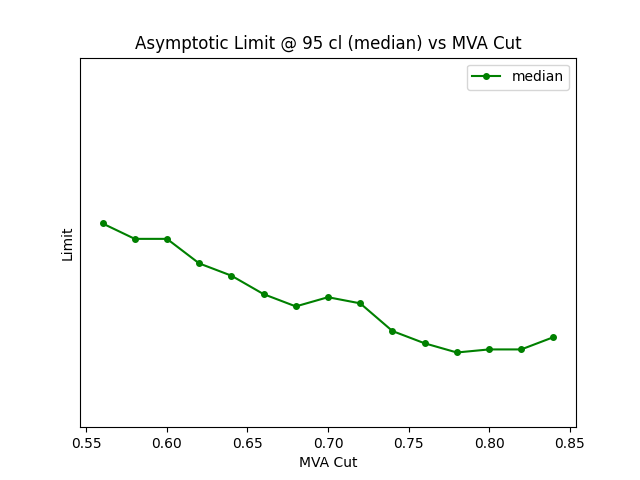
\includegraphics[width=0.45\textwidth]{figures/chapter4/results/limit_bdt_median.png}
      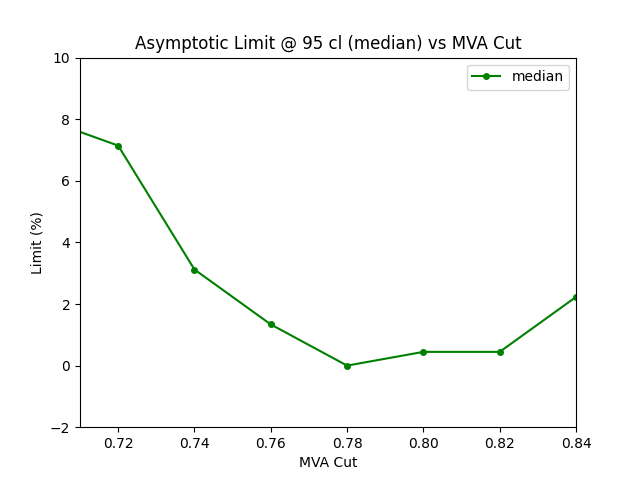
\includegraphics[width=0.45\textwidth]{figures/chapter4/results/limit_bdt_median_v2.png}\\
    \end{center}
    \caption{
      The sensitivity scan against various MVA cuts first within a broad range of MVA cut values (left) and then with a more concentrated range of MVA cut values (right).
    }
    \label{fig:sensitivity_scan}
\end{figure}

\subsection{Branching Fraction Limit}
\label{subsec:final_result}

Finally, we present the final result. After applying the formalism developed in section \ref{subsubsec:limit_calculation_theory} and unblinding the data, we find that the upper limit on the branching fraction at a $90(95)\%$ confidence level is
\begin{equation}
    \mathcal{B}(D^0 \to \mu^+ \mu^-) < 2.1(2.4) \times 10^{-9} 
\end{equation}
Table \ref{tab:final_observed_yeild} shows the central values of the observed yields for each decay channel studied in this analysis and figure \ref{fig:final_observed_fit} displays the final fit on the observed data.

\begin{table}[h!]
    \centering
    \begin{tabular}{|l|c|}
    \hline
    \textbf{Observed Yields} & \textbf{Values} \\
    \hline
    $N_{D^0 \rightarrow \mu^+\mu^-}$ & $139 \pm 123$ \\
    $N_{D^0 \rightarrow \pi^+\pi^-}$ & $220 \pm 58$ \\
    $N_{D^0 \rightarrow \pi^-\mu+\nu_\mu}$ & $207 \pm 40$ \\
    $N_{\text{comb}}$ & $126185 \pm 366$ \\
    $N_{\text{total}}$ & 126752 \\
    \hline
\end{tabular}
\caption{The final observed yield, based on data.}
\label{tab:final_observed_yeild}
\end{table}

\begin{figure}[h!]
    \begin{center}
      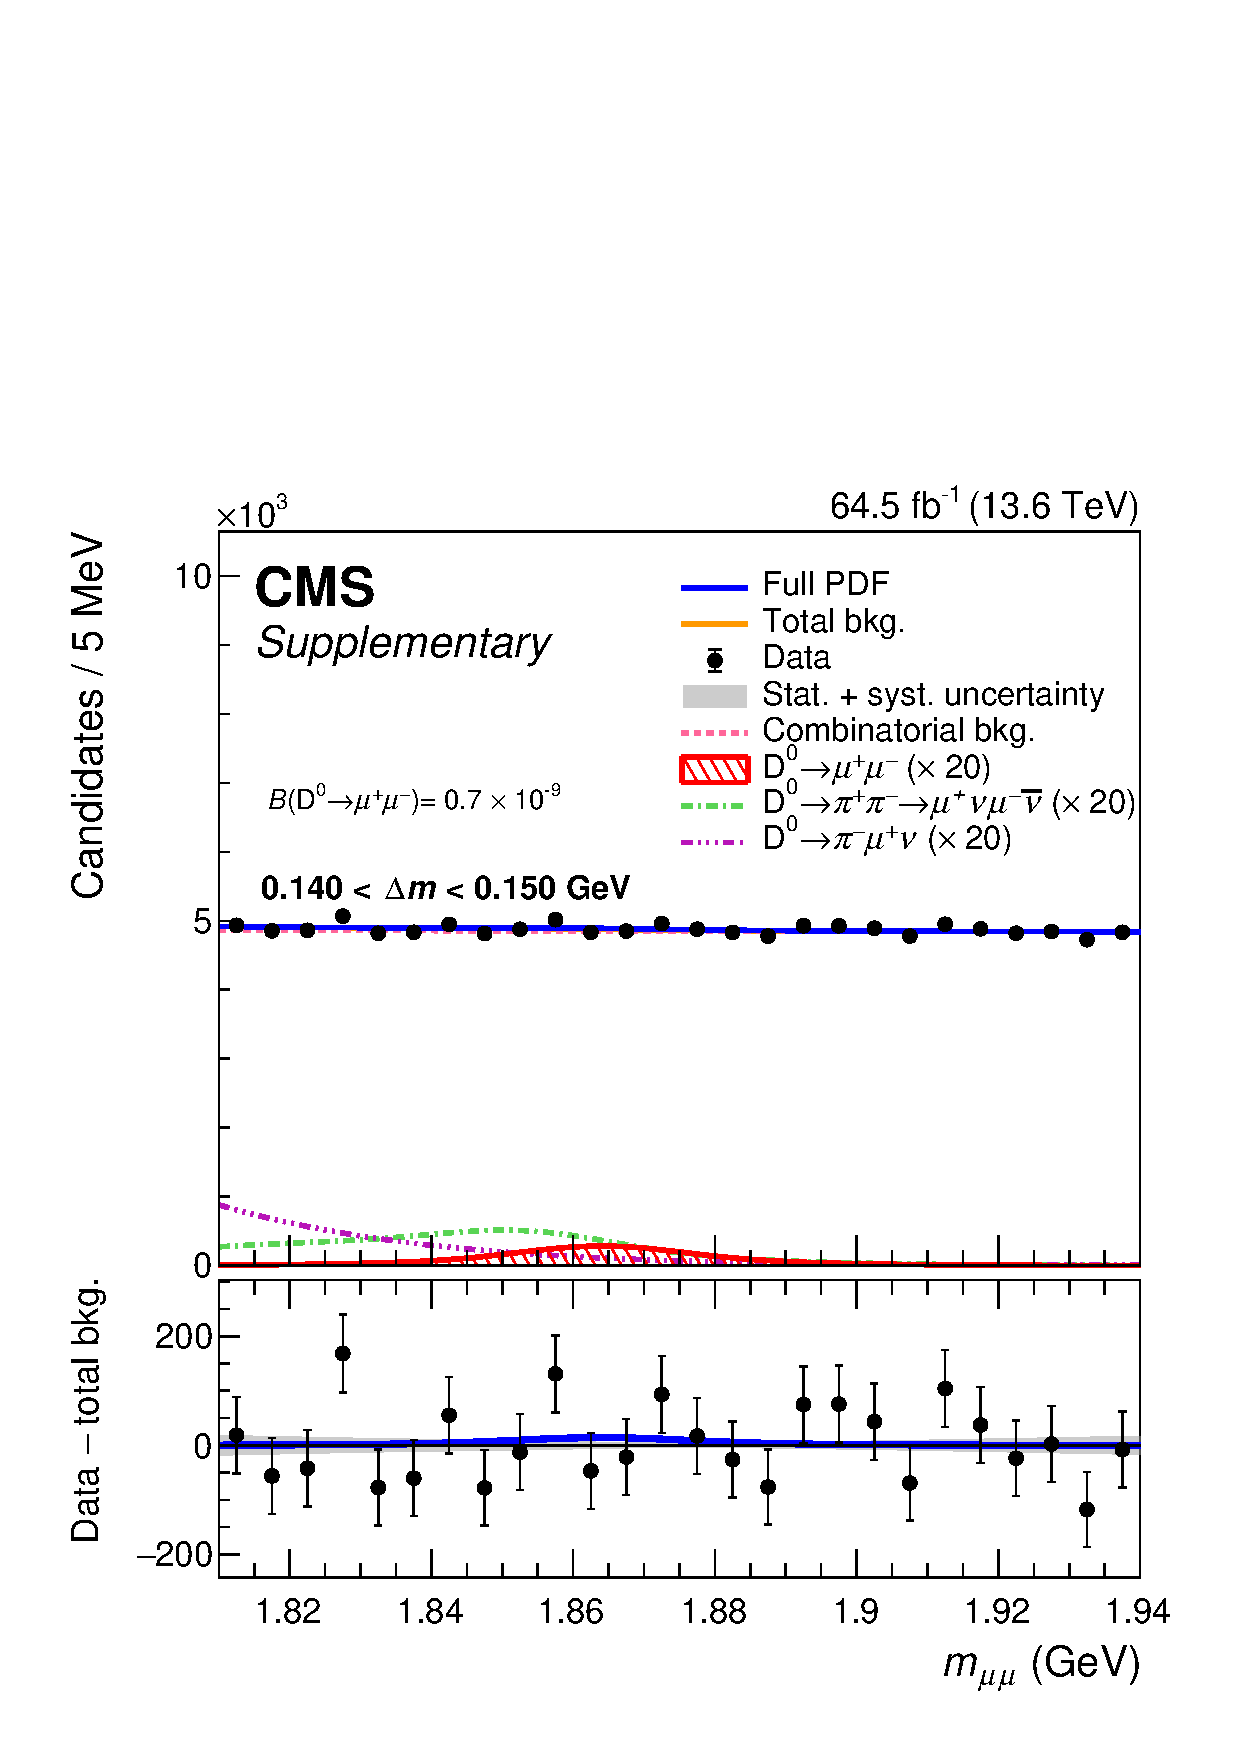
\includegraphics[width=0.45\textwidth]{figures/chapter4/results/SB_plot_m_full_test.pdf}
      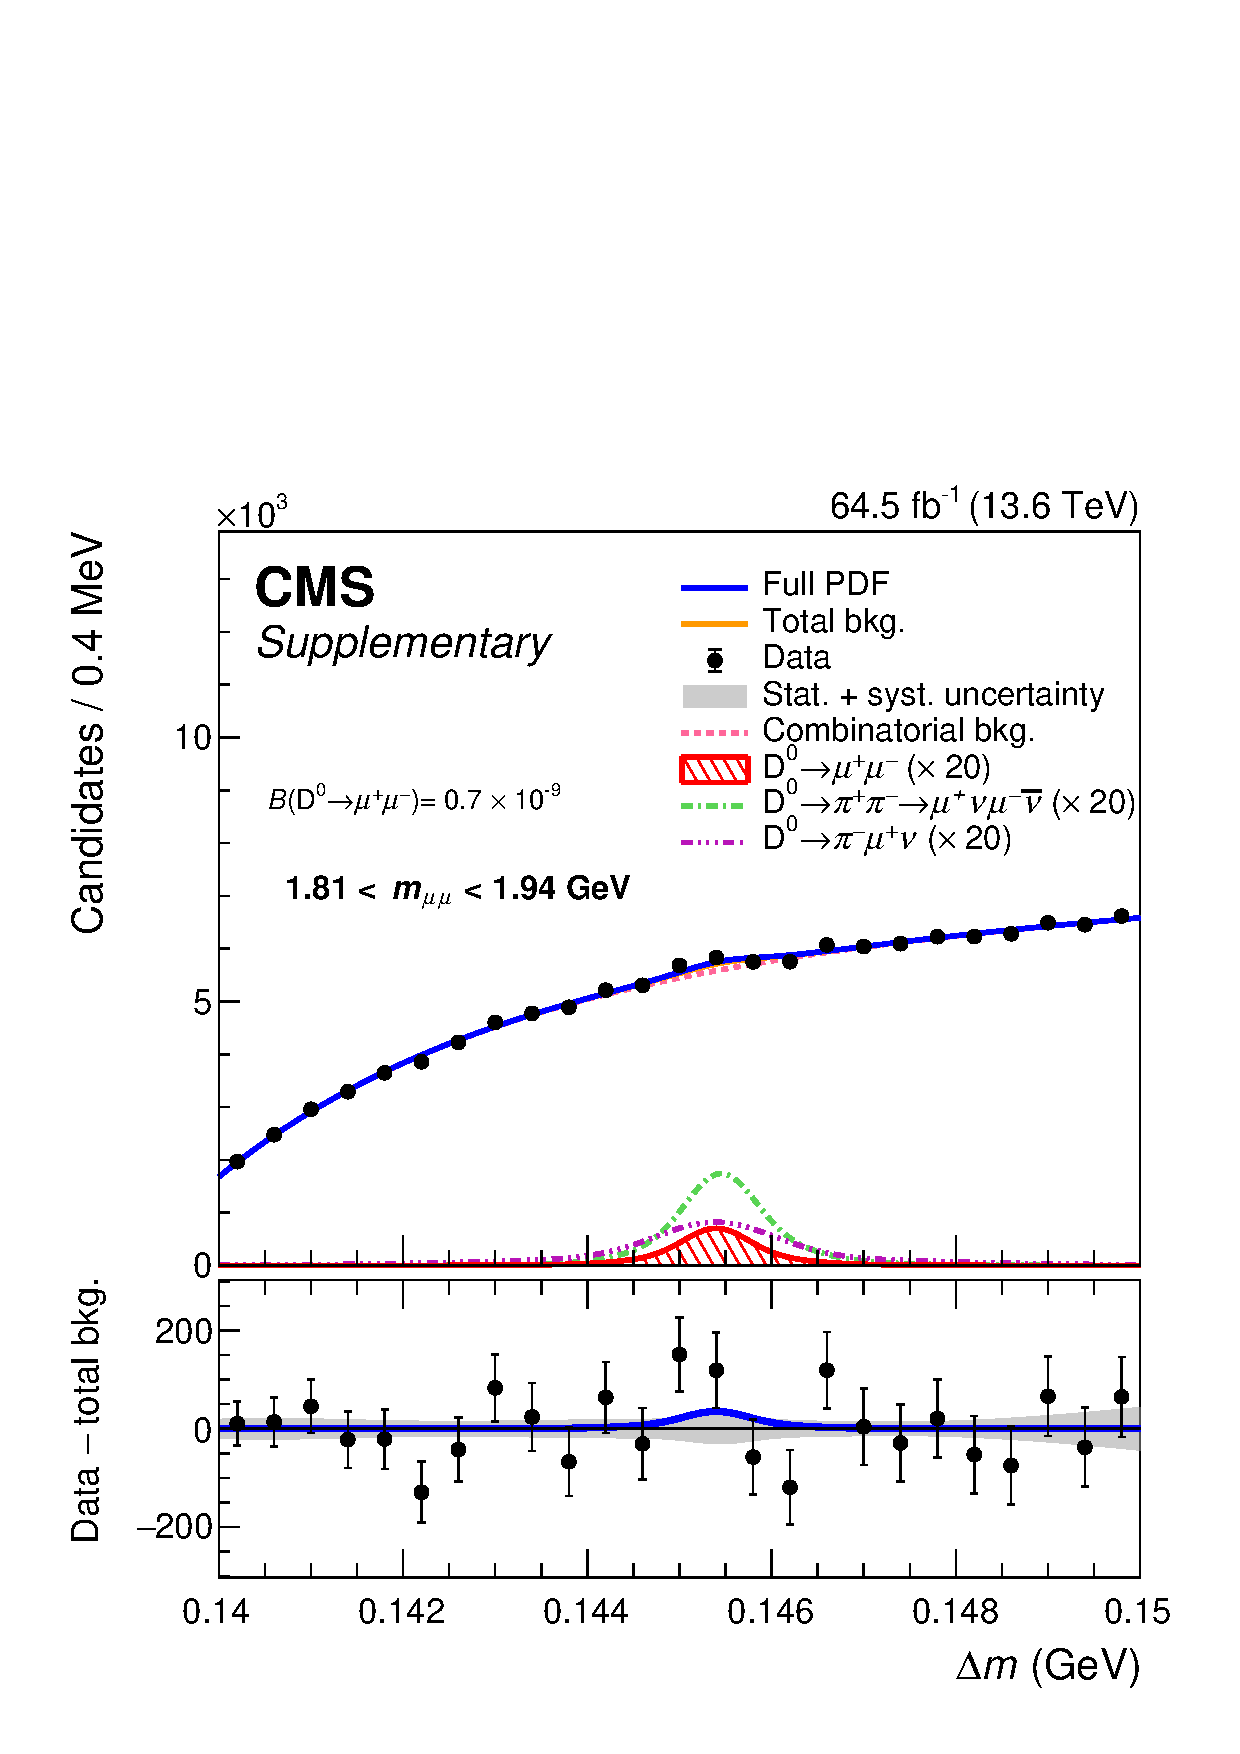
\includegraphics[width=0.45\textwidth]{figures/chapter4/results/SB_plot_dm_full_test.pdf}\\
    \end{center}
    \caption{
      The unblind fit on observed data shown in $m(D^0)$ (left) and $\Delta m$ (right). Note that the peaking decays are visually scaled by a factor of 20.
    }
    \label{fig:final_observed_fit}
  \end{figure}
\chapter{Conclusion}
\label{ch:5}

\vspace{-5mm}

A search for rare charm decays has been presented in this thesis. These rare charm decays are examples of FCNCs, which serve as excellent probes into BSM physics models due to their suppressed SM nature. Previous FCNC studies often omit charm decays and focus on strange or bottom decays. Specifically, this thesis calculated a limit on the branching fraction of the $D^0 \to \mu^+ \mu^-$ decay, denoted $\mathcal{B}(D^0 \to \mu^+ \mu^-)$. 

The analysis in this thesis had two major challenges. The first was the large amount of combinatorial background compared to the small amount of signal. The second was the presence of muon fakes, causing pions to be misreconstructed as muons and faking $D^0 \to \mu^+ \mu^-$ events. To address these obstacles, this thesis focused on $D^0$ mesons that decayed from $D^*$ mesons. This allowed for a more robust reconstruction of the signal events which kept combinatorial backgrounds low. Additionally, this thesis leveraged the well-known quantity $\mathcal{B}(D^0 \to \pi^+ \pi^-)$ to use the $D^0 \to \pi^+ \pi^-$ decay as a normalization channel. This allowed for the ability to calculate $\mathcal{B}(D^0 \to \mu^+ \mu^-)$ without actually knowing how many $D^0$ mesons were produced. Furthermore, this normalization channel caused a reduction in many systematic uncertainties, allowing for a more precise measurement. The primary data used in this analysis consisted of proton-proton collision data samples taken during 2022 and 2023 using the CMS detector at the LHC. One sample was constructed using a prescaled zero bias trigger while the other was collected using a dimuon trigger with a center of mass energy at $\sqrt{s} = 13.6$ TeV and corresponding to an integrated luminosity of $51.4\; \text{nb}^{-1}$ and $64.5\; \text{fb}^{-1}$ respectively. 

No obvious excess is observed. The final upper limit on the branching fraction at a $90(95)\%$ confidence level was found to be 
\begin{equation}
    \mathcal{B}(D^0 \to \mu^+ \mu^-) < 2.1(2.4) \times 10^{-9} 
\end{equation} 

This upper limit outperformed the previous world-best limit calculated by LHCb at a $90\%$ confidence level to be $3.1 \times 10^{-9}$ \cite{ref:lhcb_2023}, placing new constraints on BSM physics.
% TODO: add reference above and in introduction

In addition, this analysis made other key contributions in the process of deriving its final result. Namely, this analysis performed one of the most exhaustive fake rate studies to date, presenting a result and continuing development on a method which will be able to be used by many other analyses which involve muon fake rates. This analysis was also the first to use the new inclusive dimuon trigger developed at CMS. It demonstrated the benefits of the new trigger, illuminating the opportunities for its use in low-mass dimuon data. 


%%% Appendicies of thesis  %%%%%%%%%%%%%%%%%%%%%%%%%%%%%%%%%%%%%%%%%%%%%%%%%%%%%%%%%%%%%%%%%%%%%%%%

%\appendix
%% From mitthesis package
% Version: 1.01, 2023/07/04
% Documentation: https://ctan.org/pkg/mitthesis


\chapter{Code listing}

\lstdefinestyle{mystyle}{
    backgroundcolor=\color{CadetBlue!15!white},   
    commentstyle=\color{Red3},
    numberstyle=\tiny\color{gray},
    stringstyle=\color{Blue3},
    basicstyle=\small\ttfamily,
    breakatwhitespace=false,         
    breaklines=true,                 
    numbers=left,                    
    numbersep=5pt,                  
    showspaces=false,                
    showstringspaces=false,
    showtabs=false,                  
    tabsize=2
}%
\lstset{language=[5.3]Lua,style={mystyle}}%

\begin{lstlisting}
function print_rate(kappa,xMin,xMax,npoints,option)
     local c = 1-kappa*kappa
     local croot = (1-kappa*kappa)^(1/2)
     local logx = math.log(xMin)
     local psi = 0
     
     local xstep = (math.log(xMax)-math.log(xMin))/(npoints-1)
     
     arg0 = math.sqrt(xMin/c)
     psi0 = (1/c)*math.exp((kappa*arg0)^2)*(erfc(kappa*arg0)-erfc(arg0))
     
     if option~=[[]] then
  		 tex.sprint("\\addplot+["..option.."] coordinates{") 
  		 -- addplot+ for color cycle to work
     else
  		 tex.sprint("\\addplot+ coordinates{")
     end
     tex.sprint("("..xMin..","..psi0..")")
     
     for i=1, (npoints-1) do
  		 x = math.exp(logx + xstep)
  		 arg = math.sqrt(x/c)
  		 karg = kappa*arg
  		 if karg<5 then 
		 -- this break compensates for exp(karg^2), which multiplies the error in the erf approximation...
  		    logpsi = -math.log(croot) + karg^2 + math.log(erfc(karg)-erfc(arg))
  		    psi = math.exp(logpsi)
  		 else
  		    psi = (1/(karg) - 1/(2*(karg^3)) + 3/(4*(arg^5)) )/(1.77245385*croot)
  		    -- this is the large x asymptote of the reaction rate
  		 end
  		 logx = math.log(x)
  		 tex.sprint("("..x..","..psi..")")
     end
     tex.sprint("}")
end
\end{luacode*}
\end{lstlisting}



%%% Bibliography  %%%%%%%%%%%%%%%%%%%%%%%%%%%%%%%%%%%%%%%%%%%%%%%%%%%%%%%%%%%%%%%%%%%%%%%%%%%%%%%%%

%\printbibliography[title={References},heading=bibintoc]

% biblatex also supports chapter-by-chapter bibliography, https://tex.stackexchange.com/a/296502/119566
% see the biblatex manual, section 3.14.3


%%%% Option for natbib %%%%%%%%%%%%%

%%   use an appropriate style (.bst) and your own .bib file[s]

\bibliographystyle{plainnat}
\bibliography{thesis.bib}

\end{document} 
 